\documentclass[a4paper,11pt]{report}
\usepackage[T1]{fontenc}
\usepackage[utf8]{inputenc}
\usepackage[norsk]{babel}
\usepackage{graphicx}
\usepackage{multirow}
\usepackage{float}
\usepackage{subfig}
\newcommand{\HRule}{\rule{\linewidth}{0.5mm}}
\usepackage{fancyvrb}
\usepackage{pstricks}
\usepackage[pdftex]{hyperref}
\usepackage{alltt}
\usepackage{listings}
\usepackage{url}
\usepackage{SIunits}
\usepackage{subfig}
\usepackage{supertabular}
\usepackage{color}
\usepackage{geometry}

\begin{document}

\begin{titlepage}

\begin{center}
\textsc{\LARGE EiT Ecomarathon 2011}\\[1.5cm]

\HRule \\[0.4cm]
{ \huge \bfseries Prosjektrapport}\\[0.4cm]
\HRule \\[1.5cm] 

Fredrikstad, Stian\\
Gudvangen, Hans\\
Halse, Tore Egil\\
Heimark, Erlend\\
Helvig, Torgeir\\

\vfill
 
% Bottom of the page
{\large \today}

\end{center}
\end{titlepage}
%-----Innhold--------------------
\cleardoublepage
\pagenumbering{Roman}
\tableofcontents
\listoffigures
\listoftables
\clearpage
%---------------------------------
\pagenumbering{arabic}
\chapter{Henger}
\section{Gammel Løsning}
\section{Dagensløsning}
\subsection{Beskrivelse av dagens løsning}

Dagens løsning består av en skinnekonstruksjon boltet til gulvet i hengeren, og en ramme på seks hjul som ruller på denne skinnen. Se bilde under

Låsingen er en enkel mekanisme bestående av to låsepinner som treffer to hylser på baksiden av rammen, og to braketter der to skruer blir ført gjennom for så å bli låst med en bolt. Se bilde under

Rammen er også utstyrt med bein, slik at bilen kan stå på rammen, ute av bilen. Dette er en fordel om rammen skal brukes ved utstillinger og promoteringsoppdrag.  Se bilde under
\subsection{Ulemper med dagens løsning}

En av de største ulempene med dagens løsning er at rammen bilen ikke er låst i vertikalretning når bilen skal inn og ut av henger. Dette medfører en del ekstra arbeid for de involverte og er noe som Eco maraton teamet har vert misfornøyde med.

En annen ulempe er at det er vanskelig for en person å ta ned beina mens han samtidig tar ut rammen. Dette er både et praktiskproblem men det er også problematisk rent sikkerhetsmessig. 

Det er også problematisk at puten bilen ligger på under transport er for høy, slik at det blir vanskelig å få bilen inn i hengeren. Problemet ligger i at rammen puten er festet på er for høy og at bilen må presses ned av en person samtidig som bilen blir ført inn i henger av en annen.

Hjulene på rammen er et av de største irritasjonsmomentene for de daglige brukerne. Hjulene er for små og mangler nødvendig opplagring i form av solide kulelager. Rammen blir derfor eksepsjonelt vanskelig å få ut og inn av hengeren. 

\subsection{Fordeler med dagens løsning}

Den store fordelen med dagens design er at bilen kan bli fraktet i henger både med og uten hjul. Dette medfører at hjulene på bilen ikke er nær bakken under transport. Slik unngås unødvendige belastninger på hjulopphenget, som i utgangspunktet ikke tåler for mye slag, eller plutselige kraftpåkjenninger. 

En annen fordel med dagens design er at det for det meste er laget i tre, dette gjør modifikasjoner relativt enkle da alt er skrudd sammen med treskruer.

\subsection{Pris}
\subsubsection{Under 500 Nkr}
Totalt utdelt budsjett er på kr 5000. Dette er et absolutt krav
\subsection{Funksjonalitet}
\subsubsection{Opplagret for ikke å bikke}
Dagens rammekonstruksjon vil som nevnt tidligere bikke når bilens og rammens tyngdepunkt når en gitt posisjon, lenge før hele bilen er synlig ute av henger. Denne posisjonen vil Eco Maraton teamet at skal være etter at bilen har komt synlig ut av henger. Det skal være mulig å bruke hengeren med rammen til utstilling av bilen. 
\subsubsection{Lett ut og inn}
Rammen skal kunne ved hjelp av en person eller maskinkraft, bli dyttet eller dratt inn og ut av hengeren. Om det velges maskinkraft skal der være et reservesystem som gjør det samme som det maskinelle. 
\subsubsection{Enkel låsing til henger}
På grunn av liten plass i hengeren når bilen er inne er det et krav at rammen skal låsens på en enkel måte, helst uten at personer trenger gå inn i hengeren bak bilen for å låse rammen. 
\subsubsection{Enkel låsing til ramme}
Bilen skal i all hovedsak låses til rammen på utsiden av hengeren. Det blir da ikke så store tekniske krav til denne mekanismen. Et krav er uansett at dette skal kunne utføres på en enkel måte.
\subsubsection{Frakte bil uten hjul}
Rammen skal kunne bli brukt til å frakte bilen med og uten hjulene på. Dette betyr i praksis at hjulene ikke skal være i kontakt med bakken når den er festet på rammen. 
\subsubsection{Bli brukt til utstilling av bilen}
Henger med ramme skal kunne bli brukt til utstilling av bilen, i forskjellige situasjoner. Rammen må derfor være dimensjonert for både å tåle belastningene, men og på en slik måte at henger ikke bikker når bilen står på utsiden på rammen.
\section{Sikkerhet}
\subsubsection{Sikker og stabil låsing til henger}
\subsubsection{Den konstruerte låsingen på rammen til henger skal kunne stå imot harde nedbremsinger og ujevnt underlag uten at bilen tar skade av dette.  }
\subsubsection{Sikker og stabil låsing av bil}
Bilen skal kunne låses til rammen på en slik måte at den også klarer å stå imot de samme påkjennelsene som nevnt ovenfor.
\subsubsection{To personer skal kunne ta bil inn og ut av henger}
Bilen skal kunne tas ut og inn av hengeren uten hjelp av mer enn to personer. Tunge ustabile løft er mindre sikre en lette stabile løft.  
\section{Utseende}
\subsubsection{Stå i stil til bilen}
Siden rammen og hengeren skal bli brukt på utstillinger, stander osv. er det ønske at rammen har et så estetisk riktig utrykk som mulig. Helst bør rammekonstruksjonen stå i stil til resten av hengeren, og ikke minst bilen. 
\section{Vekt}
\subsubsection{Totalvekt inkludert bil under 300 kg}
På grunn av maksimal total nyttelast på hengeren på 600 kg, er det et krav at den totale vekten av både henger og bil ikke overskrider 300 kg. Dette på grunn av at det er ønskelig å frakte tilleggsutstyr i hengeren sammen med bilen.  
\section{Kompatibilitet}
\subsubsection{Kompatibel med Revolve}
Det er et ønske fra Eco maraton teamet å designe rammen på en slik måte at den enten er direkte kompatibel med bilen som Revolve teamet skal lage, eller er kompatibel etter små tilpasninger. 

\section{Ny Løsning}
\subsection{Krav fra kunde}
\begin{table}[H]
\begin{tabular}{|l|l|c|c|c|}
\hline
 & \textbf{Funksjon} & \textbf{Må} & \textbf{Bør} & \textbf{Kan} \\ \hline
\textbf{Pris} & Under 500 Nkr. & x & & \\
\hline
\multirow{6}{*}{\textbf{Funksjonalitet}} 
 & Opplagret for ikke å bikke & x & & \\
 & Lett ut og inn & x & & \\
 & Enkel låsing til henger & x & & \\
 & Enkel låsing til bil & & x & \\
 & Frakte bil uten hjul & x & & \\
 & Bli brukt til utstilling av bilen & & x & \\
\hline
\multirow{3}{*}{\textbf{Sikkerhet}}
 & Sikker og stabil låsing til henger & x & & \\
 & Sikker og stabil låsing av bil & x & & \\
 & Trengst kun to personer & & x & \\
\hline
\textbf{Utseende} & Stå i stil til bilen & &  & x \\ \hline
\textbf{Vekt} & Totalvekt inkludert bil under 300 kg & x & & \\ \hline
\textbf{Kompabilitet} & Kompatibel med Revolve & & & x \\ \hline
\end{tabular}
\caption{Funksjonskrav}
\end{table}


\subsubsection{Pris}
\begin{itemize}
\item Under 5000 Nkr \\
Totalt utdelt budsjett er på kr 5000. Dette er et absolutt krav
\end{itemize}
\subsubsection{Funksjonalitet}
\begin{itemize}
\item Opplagret for ikke å bikke \\
Dagens rammekonstruksjon vil som nevnt tidligere bikke når bilens og rammens tyngdepunkt når en gitt posisjon, lenge før hele bilen er synlig ute av henger. Denne posisjonen vil Eco Maraton teamet at skal være etter at bilen har komt synlig ut av henger. Det skal være mulig å bruke hengeren med rammen til utstilling av bilen. 
\item Lett ut og inn \\
Rammen skal kunne ved hjelp av en person eller maskinkraft, bli dyttet eller dratt inn og ut av hengeren. Om det velges maskinkraft skal der være et reservesystem som gjør det samme som det maskinelle. 
\item Enkel låsing til henger \\
På grunn av liten plass i hengeren når bilen er inne er det et krav at rammen skal låsens på en enkel måte, helst uten at personer trenger gå inn i hengeren bak bilen for å låse rammen. 
\item Enkel låsing til ramme \\
Bilen skal i all hovedsak låses til rammen på utsiden av hengeren. Det blir da ikke så store tekniske krav til denne mekanismen. Et krav er uansett at dette skal kunne utføres på en enkel måte.
\item Frakte bil uten hjul \\
Rammen skal kunne bli brukt til å frakte bilen med og uten hjulene på. Dette betyr i praksis at hjulene ikke skal være i kontakt med bakken når den er festet på rammen. 
\item Bli brukt til utstilling av bilen \\
Henger med ramme skal kunne bli brukt til utstilling av bilen, i forskjellige situasjoner. Rammen må derfor være dimensjonert for både å tåle belastningene, men og på en slik måte at henger ikke bikker når bilen står på utsiden på rammen.
\end{itemize}
\subsubsection{Sikkerhet}
\begin{itemize}
\item Sikker og stabil låsing til henger \\
\item Den konstruerte låsingen på rammen til henger skal kunne stå imot harde nedbremsinger og ujevnt underlag uten at bilen tar skade av dette.  
\item Sikker og stabil låsing av bil \\
Bilen skal kunne låses til rammen på en slik måte at den også klarer å stå imot de samme påkjennelsene som nevnt ovenfor.
\item To personer skal kunne ta bil inn og ut av henger \\
Bilen skal kunne tas ut og inn av hengeren uten hjelp av mer enn to personer. Tunge ustabile løft er mindre sikre en lette stabile løft.  
\end{itemize}
\subsubsection{Utseende}
\begin{itemize}
\item Stå i stil til bilen \\
Siden rammen og hengeren skal bli brukt på utstillinger, stander osv. er det ønske at rammen har et så estetisk riktig utrykk som mulig. Helst bør rammekonstruksjonen stå i stil til resten av hengeren, og ikke minst bilen. 
\end{itemize}
\subsubsection{Vekt}
\begin{itemize}
\item Totalvekt inkludert bil under 300 kg \\
På grunn av maksimal total nyttelast på hengeren på 600 kg, er det et krav at den totale vekten av både henger og bil ikke overskrider 300 kg. Dette på grunn av at det er ønskelig å frakte tilleggsutstyr i hengeren sammen med bilen.  
\end{itemize}
\subsubsection{Kompatibilitet}
\begin{itemize}
\item Kompatibel med Revolve \\
Det er et ønske fra Eco maraton teamet å designe rammen på en slik måte at den enten er direkte kompatibel med bilen som Revolve teamet skal lage, eller er kompatibel etter små tilpasninger. 
\end{itemize}

\section{Ny løsning}
\subsection{Flytdiagram}
\begin{flushleft}
Undersøkelse av nåværende system for transport av bil inn og ut av tilhenger, viser at det er mest hensiktsmessig å benytte seg av en rammekonstruksjon som bilen plasseres på. Rammekonstruksjonen med bilen på blir så ført videre inn i tilhengeren. Dette prinsippet er valgt å benytte videre. For å lettere få oversikt over de ulike trinnene i prosessen med å få bilen inn og ut av tilhengeren, settes det opp et flytskjema.
\end{flushleft}

\begin{figure}[h!tb]
\begin{center}
\leavevmode
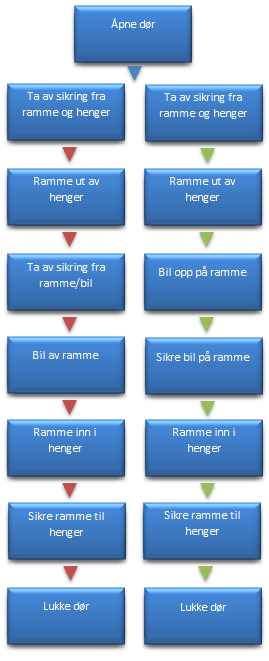
\includegraphics[width=0.4\textwidth]{images/Bildet_3}
\end{center}
\caption{Flowchart}
\label{fig:flowchart}
\end{figure}

\begin{flushleft}
Til venstre vises operasjonene med å ta bilen ut av tilhengeren, til høyre vises stegene i prosessen med å flytte bilen inn i tilhengeren.\newpage

\subsection{Morfologisk tabell}
Basert på flytdiagrammet settes det opp en morfologisk tabell. Denne er vist nedenfor.
\end{flushleft}

\begin{table}[h!]
\begin{center}
\begin{tabular}{| l | l | p{3cm} |}
\hline
\multicolumn{3}{|c|}{Morfologisk tabell} \\
\hline
\multirow{4}{*}{Flytte bil ved hjelp av} 

 & 1.1 & Plate \\
 & 1.2 & Ramme \\
 & 1.3 & Krok \\
 & 1.4 & Pute \\ \hline
\multirow{2}{*}{Inn og ut av tilhenger} 
 & 2.1 & Rulle \\
 & 2.2 & Løfte \\ \hline
\multirow{2}{*}{Drivkraft} 
 & 3.1 & Elektrisk \\
 & 3.2 & Muskelkraft \\ \hline
 \multirow{6}{*}{Forbinde drivkraft til bil} 
 & 4.1 & Vaier \\
 & 4.2 & Tau \\
 & 4.3 & Tannstang \\
 & 4.4 & Tannhjul \\
 & 4.5 & Reim \\
 & 4.6 & Direkte \\ \hline
 \multirow{4}{*}{Sikre bil til flytteanordning} 
 & 5.1 & Vaier \\
 & 5.2 & Tau \\
 & 5.3 & Stroppe \\
 & 5.4 & Mekanisk \\ \hline
 \multirow{4}{*}{Sikre flytteanordning til tilhenger} 
\multirow{4}{*}{Flytte bil ved hjelp av} 
 & 1.1 & Plate \\
 & 6.1 & Vaier \\
 & 6.2 & Tau \\
 & 6.3 & Stroppe \\
 & 6.4 & Mekanisk \\ \hline
 \multirow{8}{*}{Kontaktpunkt bil/flytteanordning} 
 & 7.1 & Flate foran \\
 & 7.2 & Flate bak \\
 & 7.3 & Flate over \\
 & 7.4 & Flate under \\ 
 & 7.5 & Sideflate \\ 
 & 7.6 & Flate over \\
 & 7.7 & Hjulbue \\
 & 7.8 & Hjuloppheng \\ \hline
\end{tabular}
\end{center}
\caption{Morfologisk tabell}
\end{table}


\subsection{Konsepter}
\begin{flushleft}
Ut ifra morfologimatrisen utvikles det 3 ulike konsepter.
\end{flushleft}

\subsubsection*{Konsept 1}
Satt sammen av følgende punkter fra Morfologisk tabell: 1.1 - 2.1 \& 2.2 - 3.2 - 4.1 - 5.3 - 6.4 - 7.4. Setter bilen opp på en liten plate slik at bilens understell hviler mot denne. Ideeen er at bilen skal transporteres inn og ut av tilhengeren mens den står oppe på platen. Platen med bilen på skal løftes inn i tilhengeren ved hjelp av vaiere. Vaierne er festet til to skinner som kan draes inn og ut av tilhengeren. Skinnene draes ut og vaierne senkes ned og hektes fast i platen. Platen og bilen heises så opp og skinnen skyves inn i tilhengeren. Platen sikres så til tilhengeren slik at bilen står tygt under transport. Motsatt prosedyre når bilen skal ut av tilhengeren. Dette konseptet krever at bakdøren i tilhengeren hengsles om slik at den åpnes sideveis istedet for nedover.

\begin{figure}[h!tb]
\begin{center}
\leavevmode
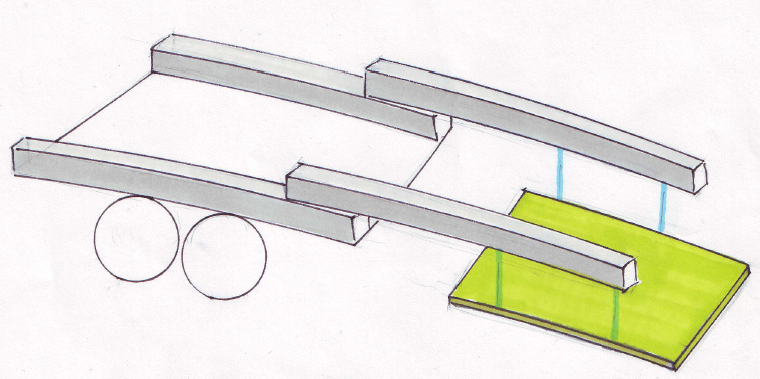
\includegraphics[width=0.6\textwidth]{images/Bildet_5}
\end{center}
\caption{Konsept 1}
\label{fig:Konsept 1}
\end{figure}

\subsubsection*{Konsept 2}
Satt sammen av følgende punkter fra Morfologisk tabell: 1.2 \& 1.4 - 2.1 - 3.2 - 4.1 - 5.3 - 6.4 - 7.4. I dette konseptet settes bilen først opp på en ramme som det er festet hjul under. Oppe på rammen skal undersiden av bilen hvile mot en pute, slik som på dagens løsning. Denne rammen skal så draes opp tilhengerdøren bak og inn i tilhengeren ved hjelp av en vaier som blir drevet av en manuell vinsj. Dette konseptet krever at hjulene på rammen er montert helt foran og bak slik at denne ikke tar nedi. Det må også monteres noen hjul på tilhengerkanten som rammen kan rulle på når den skal over kanten. Ellers vil den ta nedi også her.

\begin{figure}[h!tb]
\begin{center}
\leavevmode
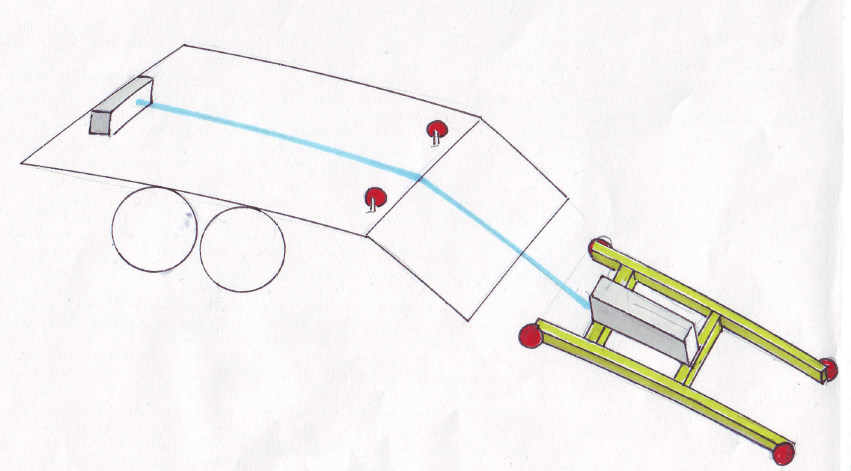
\includegraphics[width=0.6\textwidth]{images/Bildet_4}
\end{center}
\caption{Konsept 2}
\label{fig:Konsept 2}
\end{figure}

\subsubsection*{Konsept 3}
Satt sammen av følgende punkter fra Morfologisk tabell: 1.2 - 2.1 \& 2.2 - 3.2 - 4.6 - 5.3 - 6.4 - 7.4. I likhet med Konsept 2 settes bilen opp på en ramme slik at understellet hviler mot en pute. Under rammen er det montert hjul på samme måte som i Konsept 2. Rammen skyves opp tilhengerdøren bak og inn i tilhengeren ved hjelp av direkte manuell kraft.  Det monteres hjul på tilhengerkanten som rammen kan rulle på når den skal over denne. For å hindre at rammen skal ``tippe'' når bilen skal tas ut av tilhengeren og rammen kommer et stykke utover kanten på tilhengeren, skal det monteres en ``støttebrakett'' på hver side av rammen. Denne skal hindre at rammen tipper ned, inntil den har kommet en viss lengde ut av tilhengeren. På denne måten blir rammen enklere å kontrollere og sikkerheten ivaretas på en bedre måte.

\begin{figure}[h!tb]
\begin{center}
\leavevmode
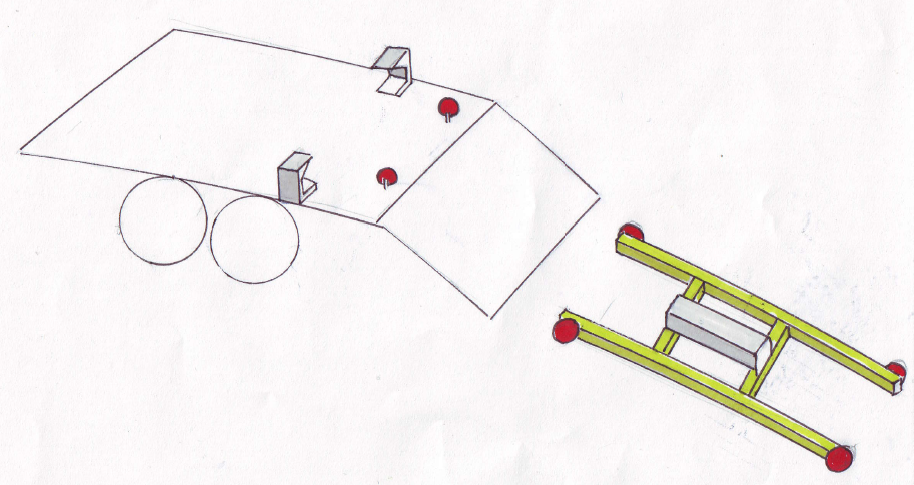
\includegraphics[width=0.6\textwidth]{images/Bildet_6}
\end{center}
\caption{Konsept 3}
\label{fig:Konsept 3}
\end{figure}

\subsection{Evaluering og valg av konsept}
Evaluerer de tre konseptene opp mot hverandre ved å sette de inn i en evalueringsmatrise. Ulike egenskaper blir vektet med poengsum fra 1 til 4, hvor en er dårligst og 4 er best. De ulike konseptene blir så gitt poeng fra 1 til 3 etter hvor gode de er på de ulike genskapene. 1 er dårligst og 3 er best. Til slutt blir vektingen av egenskapene addert med poengene og summert sammen. Det konseptet med høyest totalsum er det beste.

\begin{table}[h!]
\begin{center}
\begin{tabular}{| l | c |c | c | c |}
\hline
\multicolumn{5}{|c|}{Evalueringsmatrise} \\
\hline
\textbf{Egenskap} & \textbf{Vekting} & Poeng Konsept 1 & Poeng Konsept 2 & Poeng Konsept 3\\
\hline
Lav kompleksitet & 2 & 1 & 3 & 3\\
\hline
Lav pris &4 & 1 & 2 & 2\\
\hline
Brukervennlighett & 4 & 3 & 1 & 2\\
\hline
Lav vekt & 3 & 1 & 3 & 3\\
\hline
Kvalitet & 4 & 3 & 2 & 2\\
\hline
Modifiserbar & 1 & 1 & 3 & 3\\
\hline
Funksjonalitet & 4 & 3 & 2 & 2\\
\hline
\multicolumn{2}{|l|}{Total poengsum} & 46 & 46 & 50 \\
\hline
\end{tabular}
\end{center}
\caption{Evealueringsmatrisel}
\end{table}

\begin{flushleft}
Ser at Konsept 3 får høyest poengsum, det velges derfor å gå videre med dette konseptet.
\end{flushleft}


\subsection{3D-modeller}
Det valgte konseptet blir så i sin helhet modellert i 3D. Konseptet har fokus på funksjonalitet, ikke nødvendigvis design. Figur \ref{F1} viser hele sammenstillingen. 

\begin{figure}[H]
\centerline{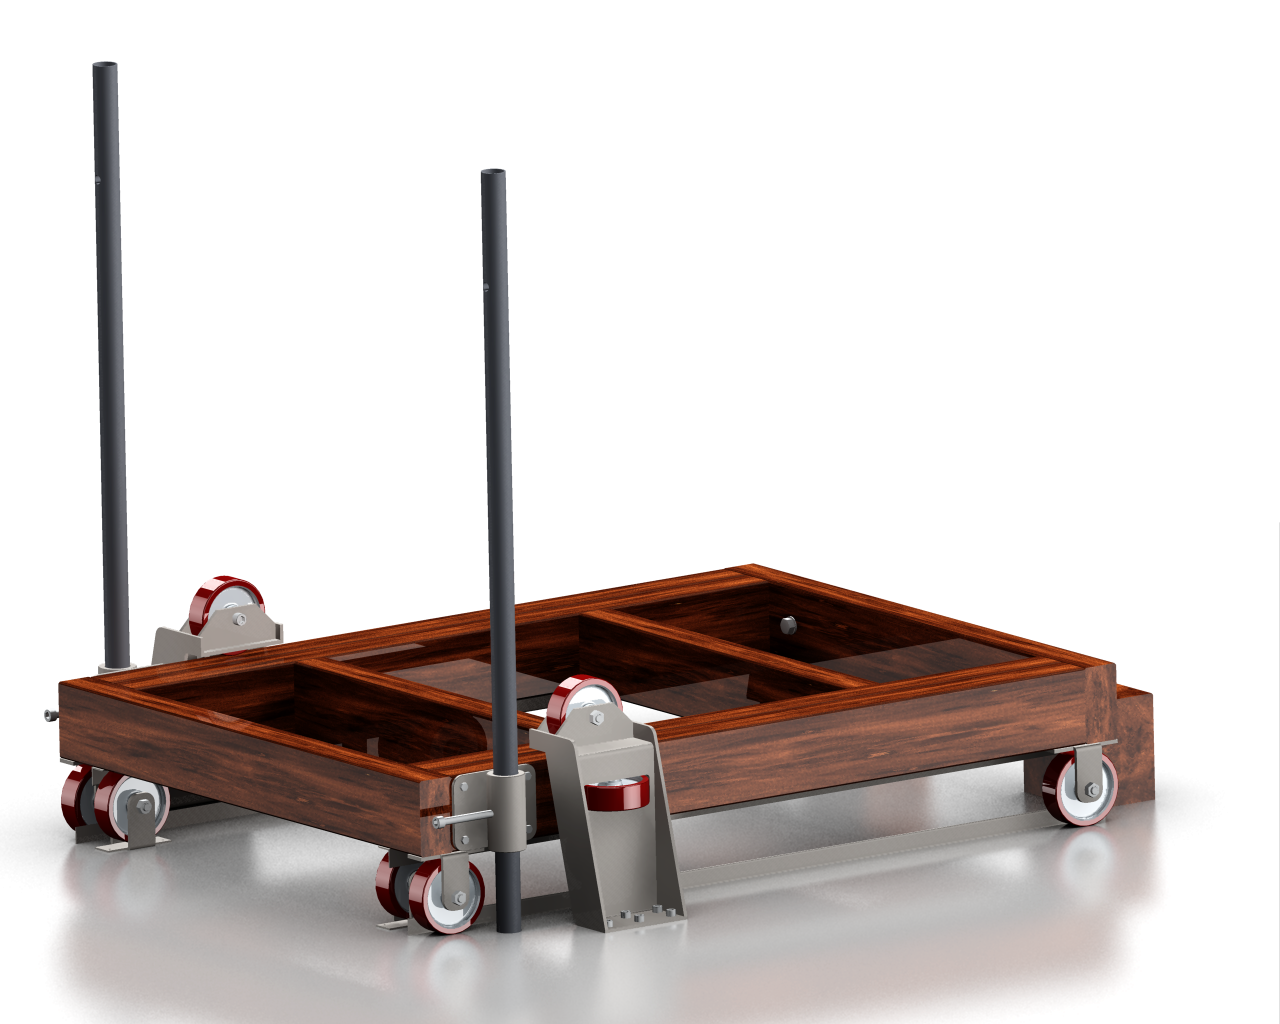
\includegraphics [width=15cm]{images/1.png}}
\caption{Sammenstilling}
\label{F1}
\end{figure}

\subsubsection{Rammen}
Den trefargede rammen er ikke modlert i full skala, dette for å gjøre det enklere å se detaljene. 
Rammen står på fire hjul. Disse hjulene hviler på gulvplanet i hengeren. Samtidig er det skrudd to hjul på selve hengerplanet, for å støtte rammen når den blir ført opp på skråplanet og videre inn i hengeren. Se Figur \ref{F1}. Selve rammen er den samme som brukt tidligere, og er som Figur \ref{F1} antyder laget av tre. På undersiden av rammen er det skrudd fast to vinkelstål som Figur \ref{F2} viser. Disse blir brukt for å lede hjulene montert på hengerplanet slik at de treffer rammen i korrekt posisjon. 
Det er også festet to vinkelstål på selve hengerplanet. Disse er, i likhet med de på rammen, ment for å lede hjulene på rammen i korrekt posisjon.
 
\begin{figure}[H]
\centerline{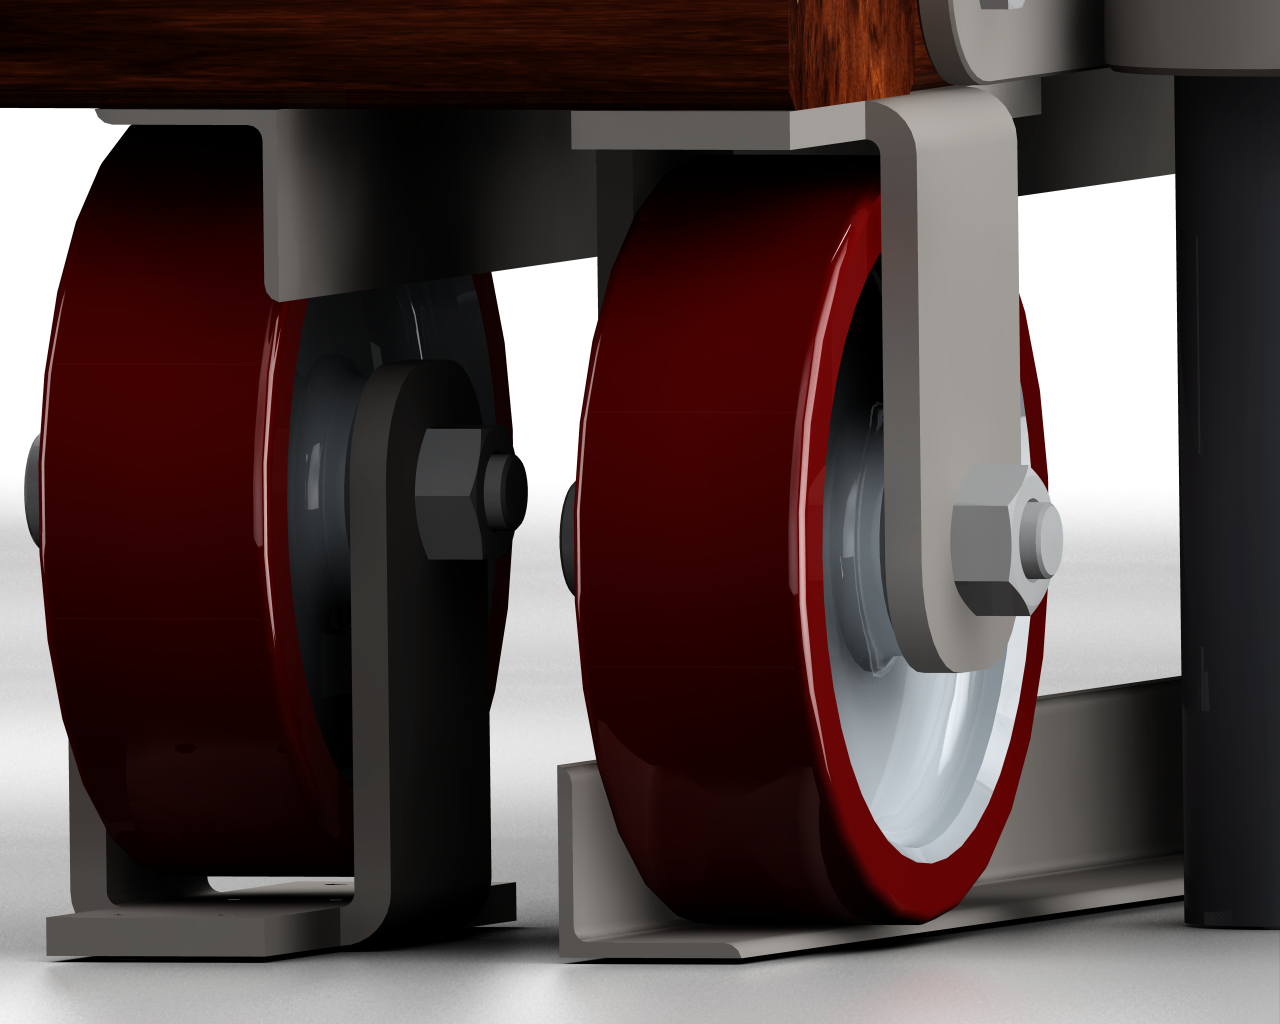
\includegraphics [width=13cm]{images/9.png}}
\caption{Vinkelstål}
\label{F2}
\end{figure}

\subsubsection{Hjulbraketter}

Hjulbrakettene er utformet sm Figur \ref{F3} viser. Disse er utformet i stålkvalitet S355J0. 
Hjulene blir festet til hjulbrakettene med M10 sylinderskruer og låsemuttere. Brakettene blir festet både til rammen og til hengerplanet ved hjelp av enkle treskruer. Hjulene er primært utsatt for trykk, svært små bøyekrefter. Dette gjør det forsvarlig å fetste disse på denne måten. Hvert hjul har en oppgitt bærekappasitet på 125 kg 

\begin{figure}[H]
\centering   
\subfloat[Hjulbrakett Venstre]{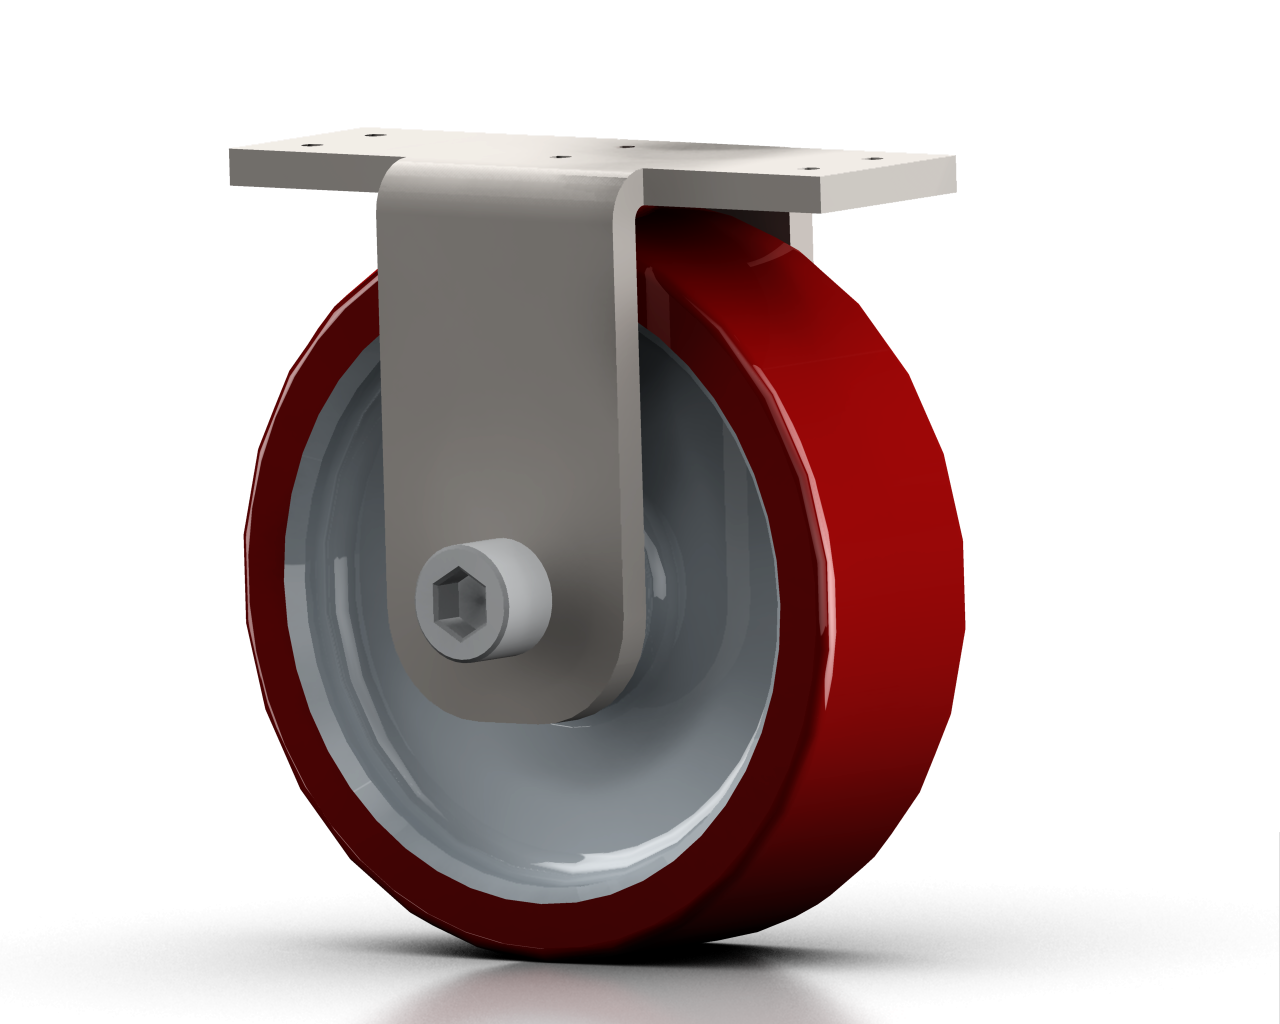
\includegraphics[width=0.5\textwidth]{images/4.png}}
\subfloat[Hjulbrakett Høyre]{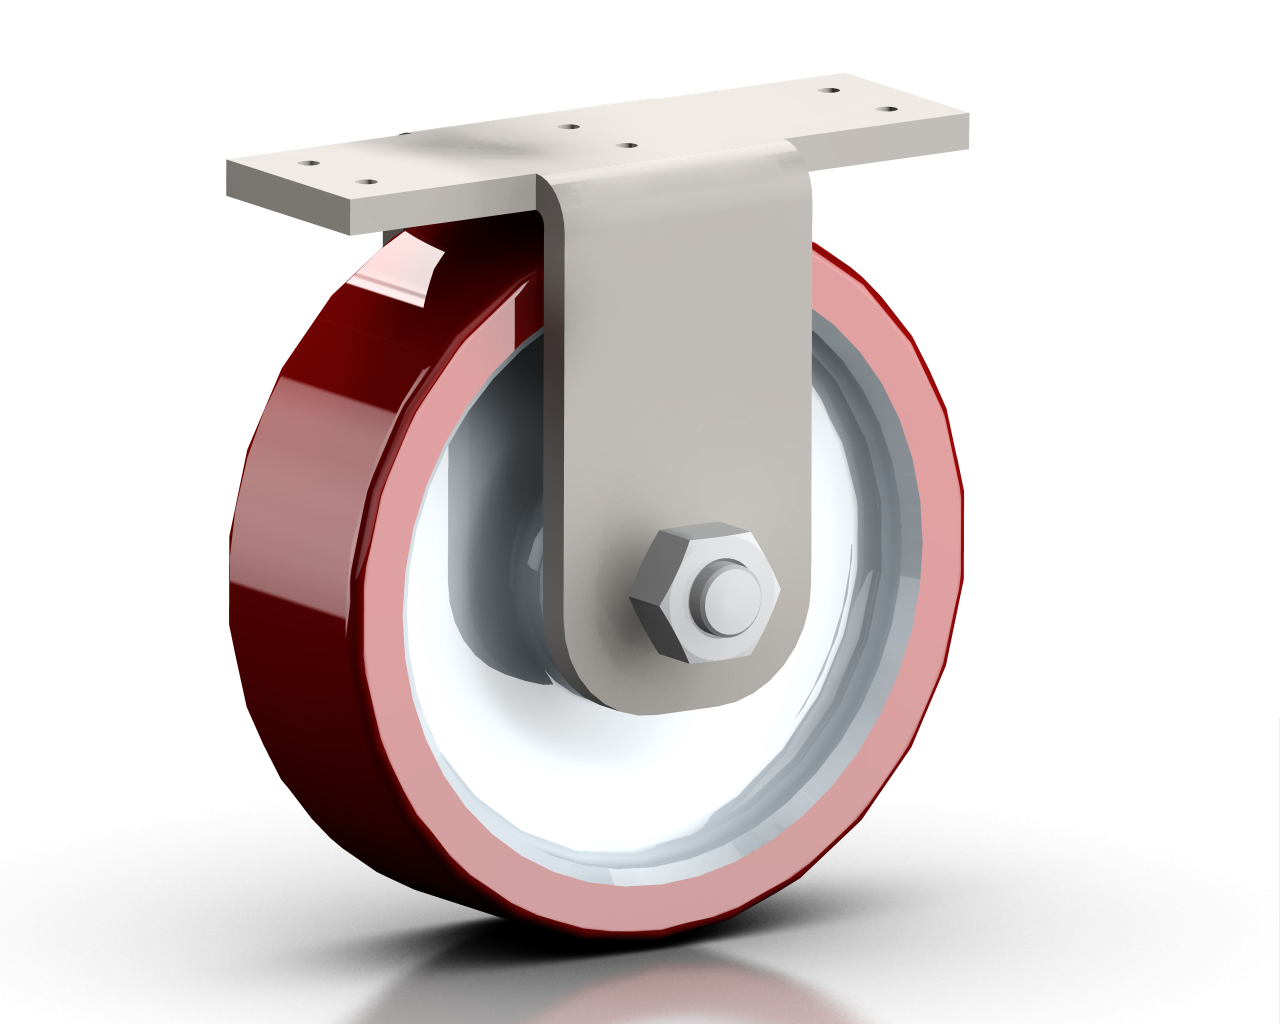
\includegraphics[width=0.5\textwidth]{images/5.png}}
\caption{Hjulbrakett}
\label{F3}
\end{figure}

\subsubsection{Støttebraketter}

Støttebralkettene skal utformes som vist i Figur \ref{F4}. Stålkvaliteten er også for disse S355J0. Platene er laserkuttet og sveist sammen med TIG på utsidene, buttsveiser, og MIG på innsidene, kilsveiser. Hjulene er laget av plastikk, med gummihjulbaner og er opplagret med kulelager. Hjulene som er benyttet er de samme som på hjulbrakettene.

\begin{figure}[H]
\centering   
\subfloat[Støttebrakett forrfra]{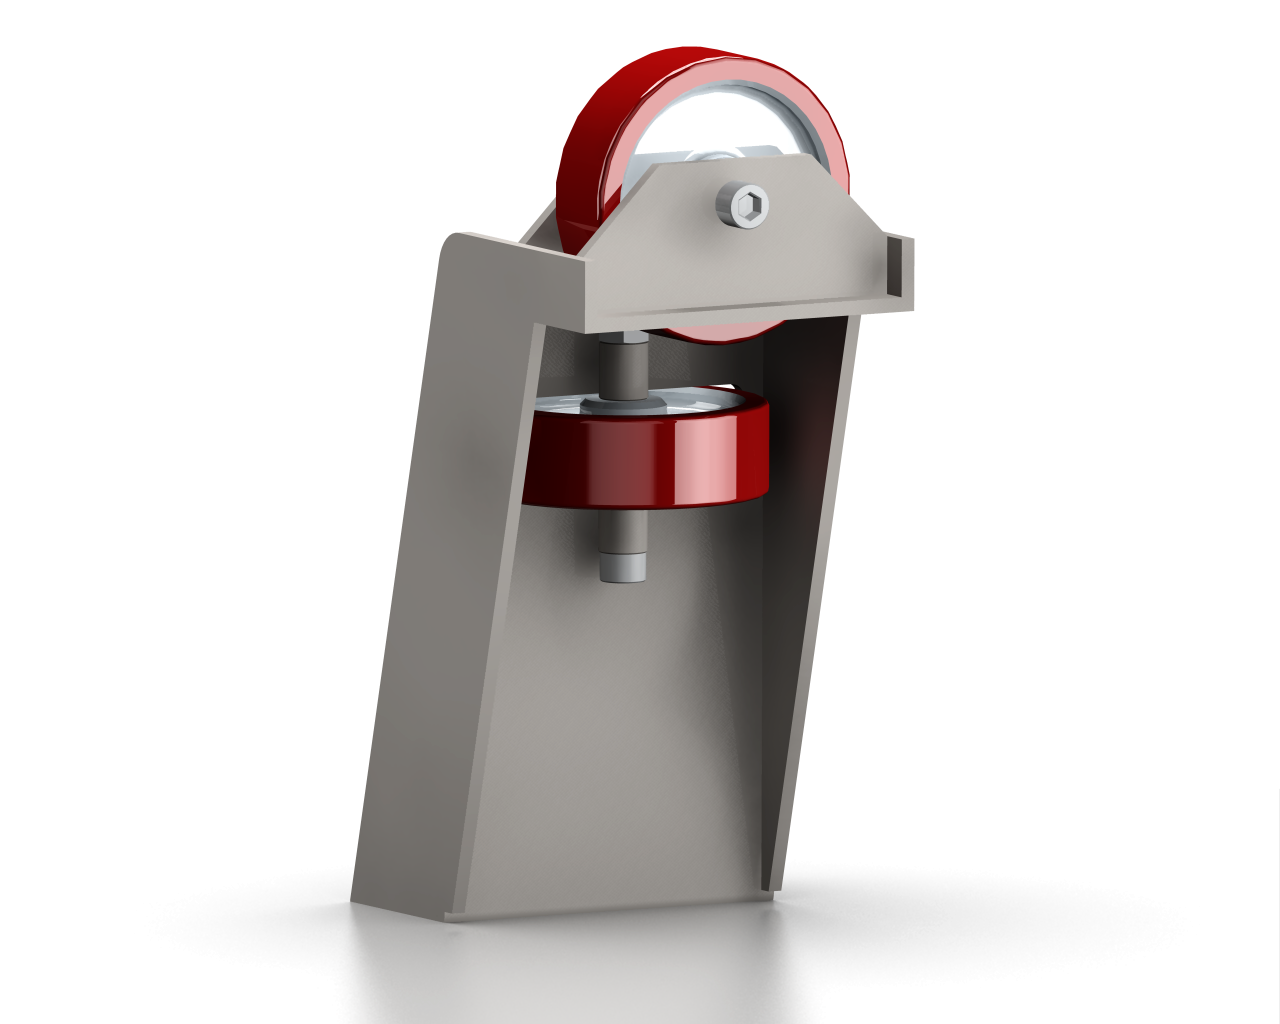
\includegraphics[width=0.5\textwidth]{images/3a.png}}
\subfloat[Støttebrakett bakfra]{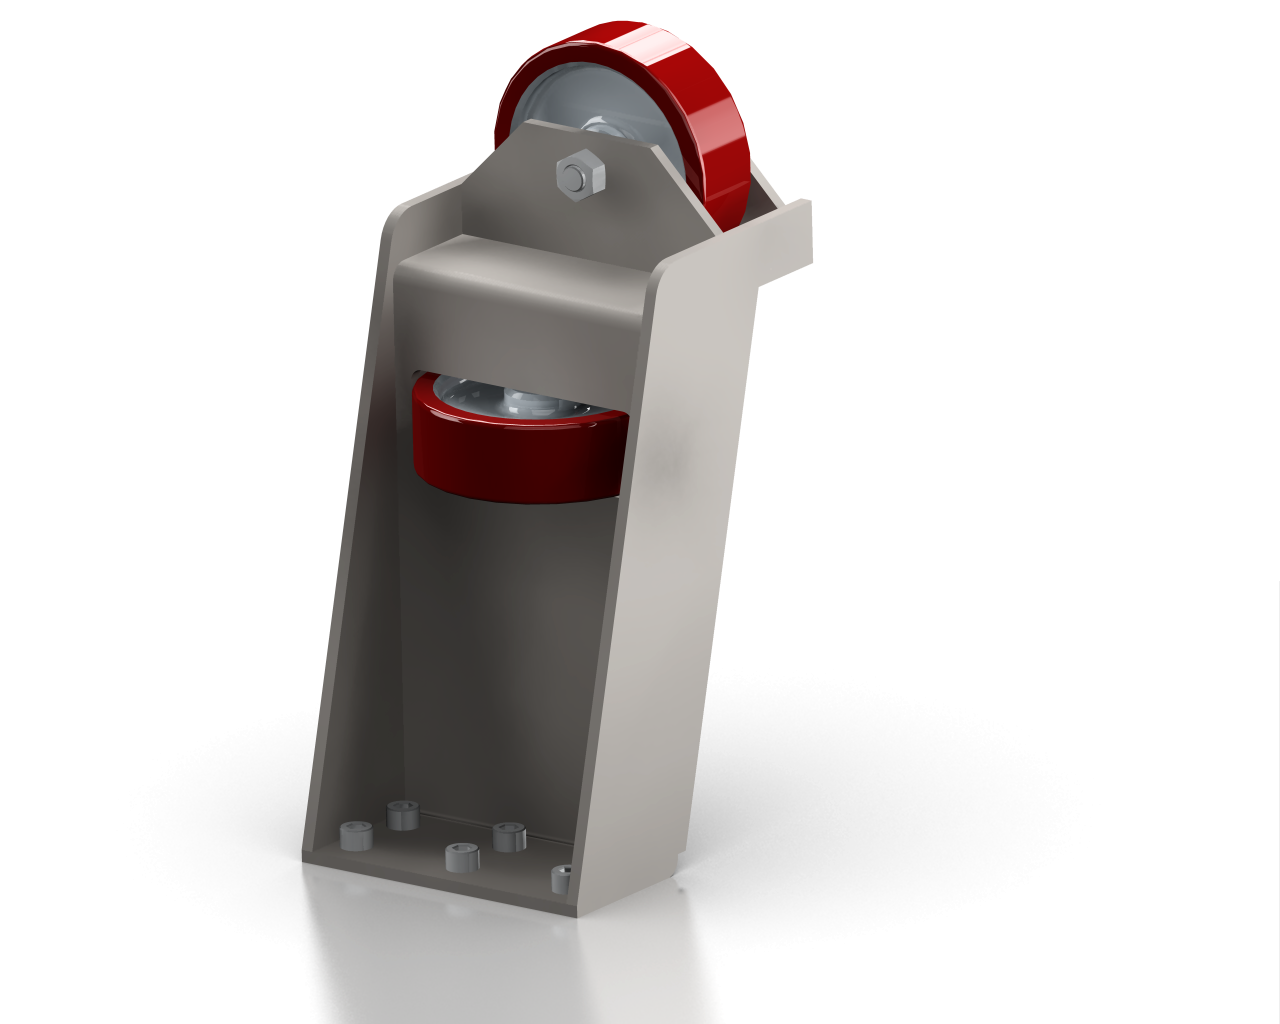
\includegraphics[width=0.5\textwidth]{images/3b.png}}
\caption{Støttebrakett}
\label{F4}
\end{figure}

Det skal benyttes M10 sylinderskruer med kvalitet 12.9 på alle hjulene. Videre skal selve braketten festet til hengeren med 6 stk, M6 syliderskruer, her også med kvalitet 12.9.    

\subsubsection{Støttebein og låsing}

Som Figur \ref{F5} viser er det designet to foringer som holder to rør. Disse rørene er ment som støtte for rammen når den blir brukt til utstilling av bilen. Altså når rammen er ute av henger mens bilen står på rammen. For mer detaljer se vedlagte arbeidstegninger og sammenstillingstegninger. Beina har både funksjon som støtte, men også som låsing i lengderetning på hengeren. Når rammen skal låses senkes beina ned på to tapper, som er boltet fast fra undersiden av hengeren. Rammen låses dermed i alle retninger. Se Figur \ref{F5}.

\begin{figure}[H]
\centering   
\subfloat[Støtteben]{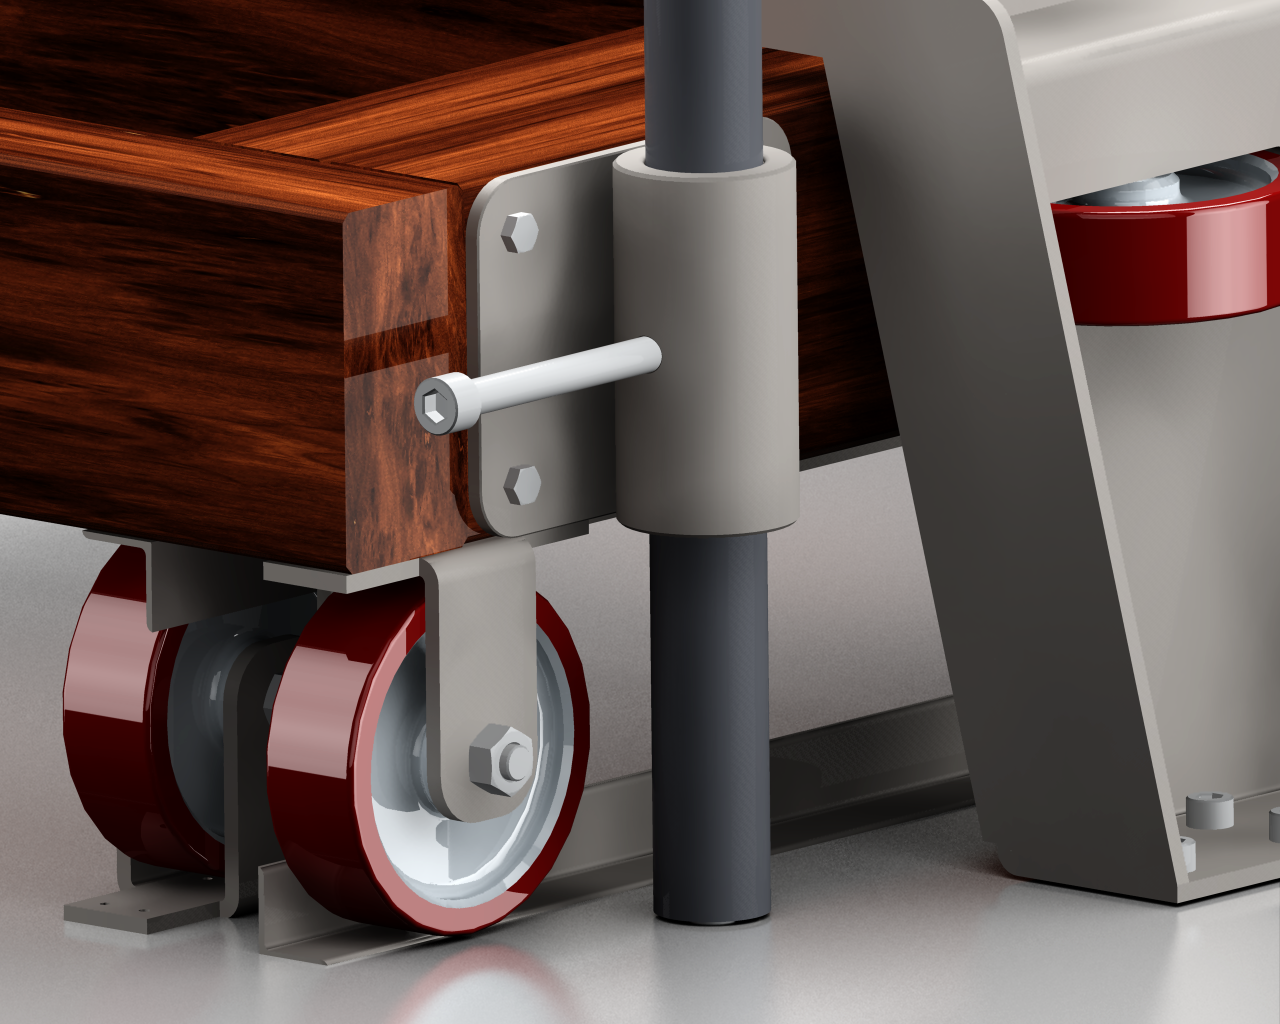
\includegraphics[width=0.4\textwidth]{images/6.png}}
\qquad
\subfloat[Låsetapp]{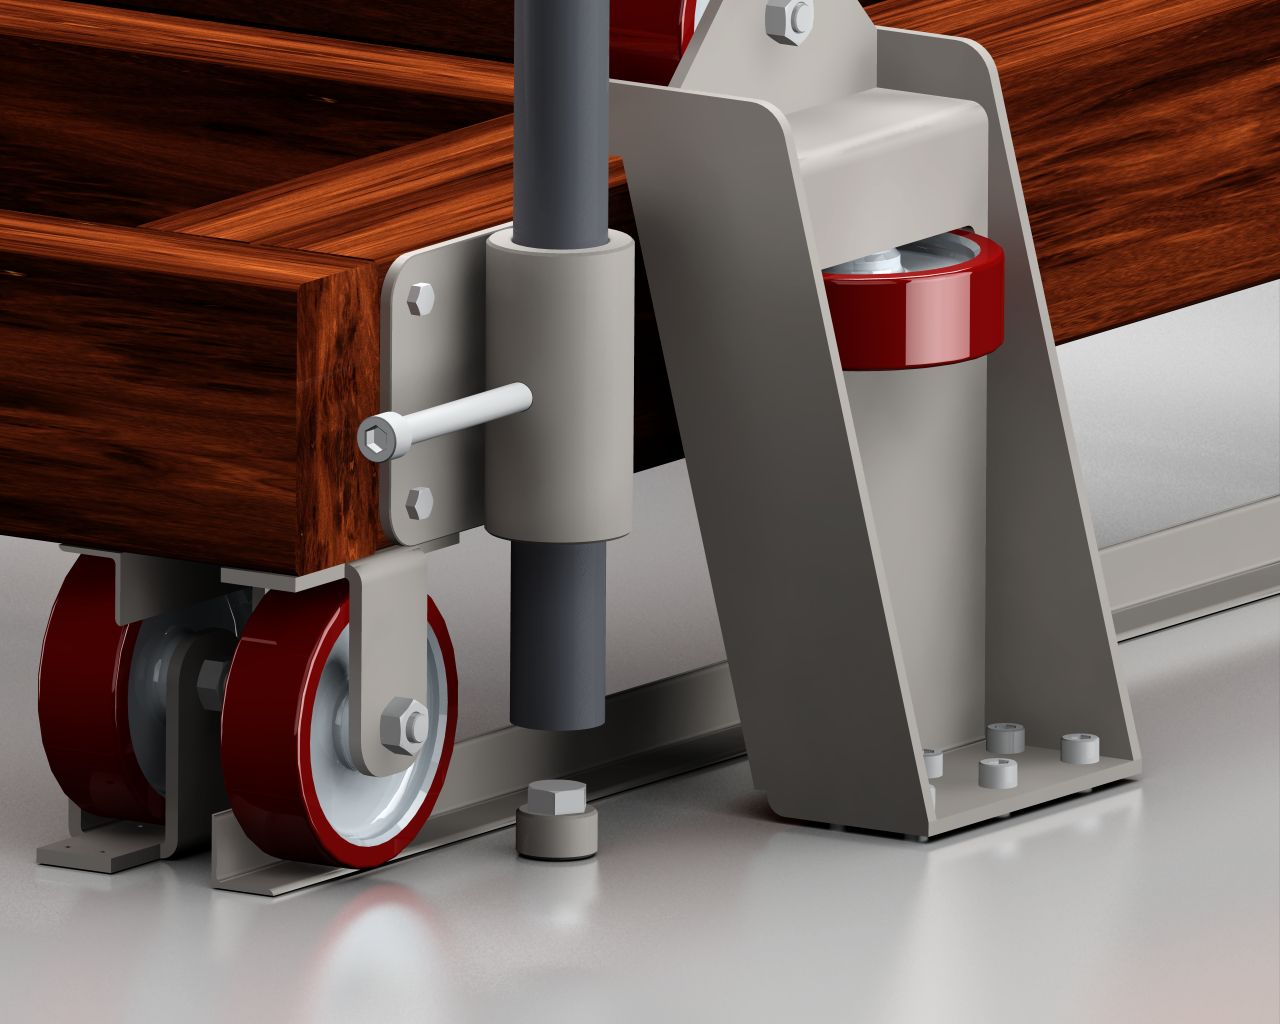
\includegraphics[width=0.4\textwidth]{images/7.png}}
\caption{Støtteben og låsing}
\label{F5}
\end{figure}

På baksiden av rammen er det festet to låsetapper. Se Figur \ref{F6}. Disse tappene har i likhet med beina funkjon som låsing. Når rammen føres inn i hengeren vil disse tappene treffe to rør som er festet til en brakett. Rammen blir slik også låst fra baksiden.  

\begin{figure}[H]
\centerline{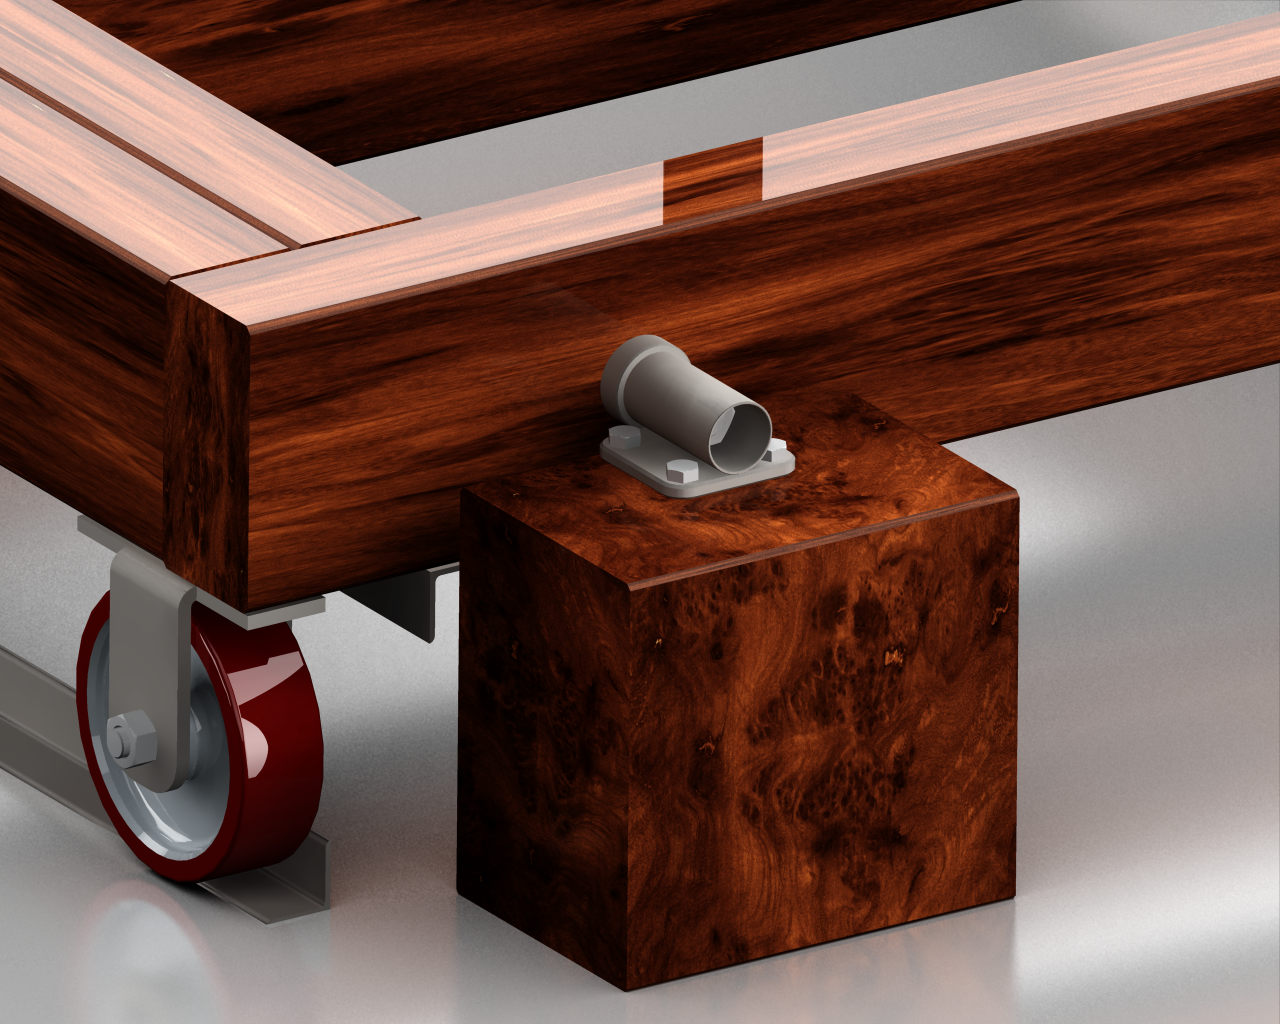
\includegraphics[width=7cm]{images/8.png}}
\caption{Låsetapper}
\label{F6}
\end{figure}

\section{Beregning av opplagerkrefter}
Det er nødvendig å bestemme kreftene som opptrer i rammens opplager for å kunne verifisere designet


\begin{figure}[H]
\begin{center}
\leavevmode
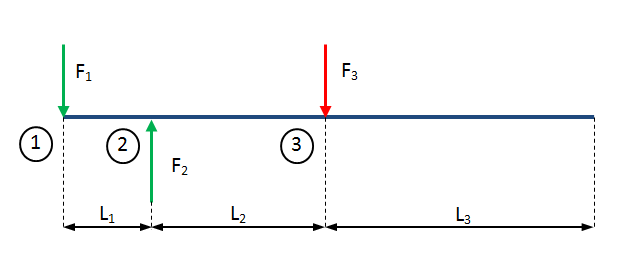
\includegraphics[width=0.8\textwidth]{images/Bilden_1}
\end{center}
\caption{Krefter ramme}
\label{fig:Krefter}
\end{figure}


Kraften $F_3$ tilsvarer halvparten av bilens vekt, siden den blir fordelt på rammens to sider. I denne rapporten er det beregnet med en vekt på bilen tilsvarende 100 kg. Det er videre antatt at denne kraften virker midt på rammen (bilens tyngdepunkt på midten). Rammens egenvekt er neglisjert. \\



Momentlikevekt om Punkt 1:

\begin{equation}
\sum{M_1}=0
\end{equation}

\begin{equation}
F_3(L_1+L_2)-F_2\cdot L_1=0
\end{equation}
 
\begin{equation}
F_2=\frac{F_3(L_1+L_2)}{L_1}
\end{equation}

\begin{equation}
F_2=\frac{F_3(L_1+L_2)}{L_1}
\end{equation}\\\\

Kraftlikevekt i Y-retning:


\begin{equation}
\sum{F_Y}=0
\end{equation}

\begin{equation}
F_2-F_1-F_3=0
\end{equation}

\begin{equation}
F_2-F_1-F_3=0
\end{equation}
 
\begin{equation}
F_1=F_2-F_3
\end{equation}


\begin{equation}
F_1=\frac{F_3(L_1+L_2)}{L_1}-F_3
\end{equation} \\

Graf som viser forholdet mellom $L_1$ og opplagerkreftene $F_1$ og $F_2$:

\begin{figure}[H]
\begin{center}
\leavevmode
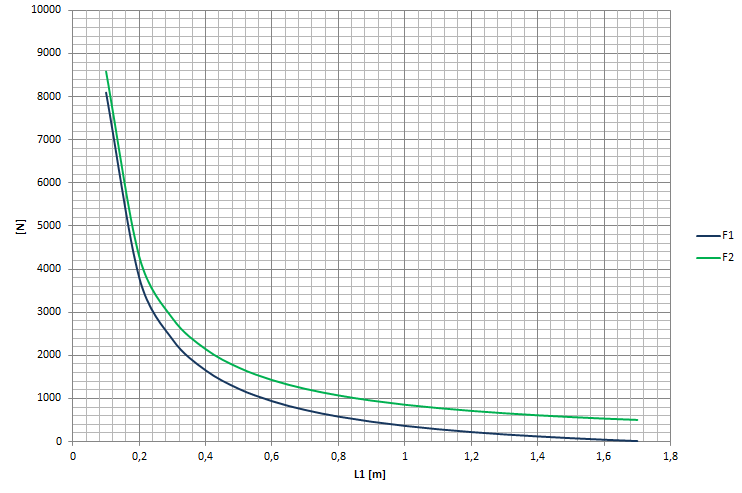
\includegraphics[width=1.0\textwidth]{images/Bilden_2}
\end{center}
\caption{$F_1$ og $F_2$ som en funksjon av $L_1$}
\label{fig:Krefter}
\end{figure}

Setter minste verdi av $L_1$ lik 0.5 m. Vil da få opplagerkrefter på $F_1$ lik 1230 N og $F_2$ lik 1720 N. Dette er de største opplagerkreftene som kan oppstå, og det er disse verdiene som brukes videre i styrkeberegningene.



\section{Styrkeberegning}
\subsection{Hjulbrakett}
Dette gjøres i UGS NX Nastran 7.5, Advanced Simulation. Kraften F2 = 1720 N fordeles likt over de to hullene i hjulbraketten. Hjulbraketten settes som fast låst på undersiden.

\begin{figure}[H]
\begin{center}$
\begin{array}{ccc}
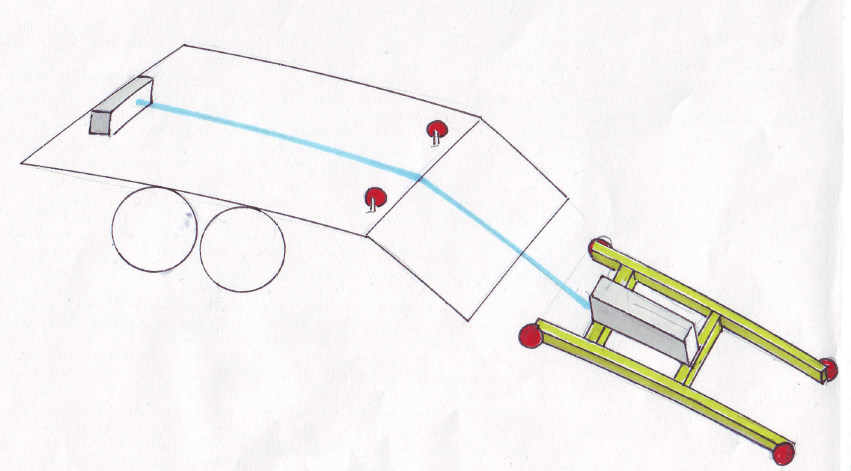
\includegraphics[width=2.5in]{images/Bilde_4.PNG} &
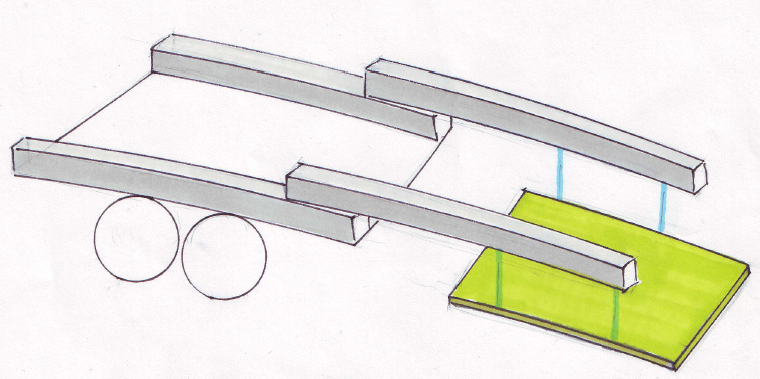
\includegraphics[width=2.5in]{images/Bilde_5.PNG} &  
\end{array}$
\end{center}
\caption{Krefter og grensebetingelser hjulbrakett}
\end{figure}

Kjører simuleringen og får største spenning $\sigma_{max}$=105 MPa. Ser at denne vil oppstå i opplagerhullet til hjulets aksel, på den siden hvor skruehodet er forsenket.

\begin{figure}[H]
\begin{center}$
\begin{array}{ccc}
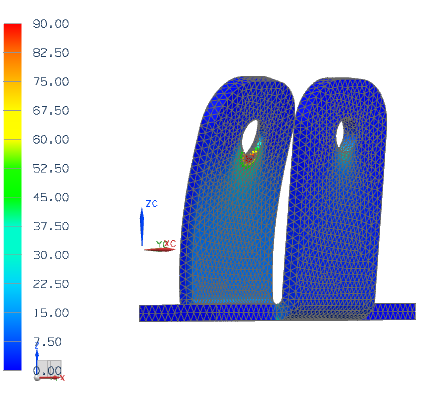
\includegraphics[width=2.0in]{images/Bilde_2.PNG} &
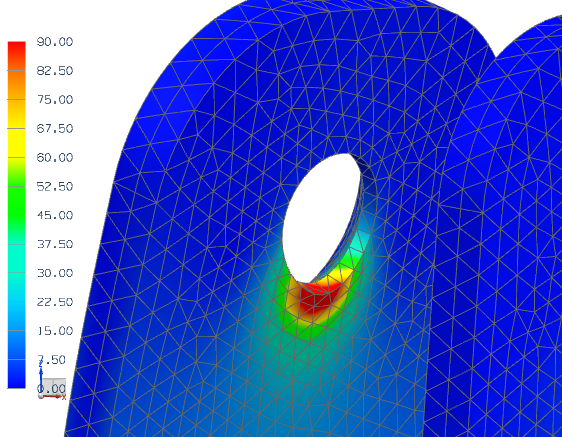
\includegraphics[width=2.0in]{images/Bilde_3.PNG} &  
\end{array}$
\end{center}
\caption{Von-Mises spenninger hjulbrakett}
\end{figure}

Ståltype S235JR som benyttes har flytgrense $\sigma_{ys}$=225 MPa. Kan ut ifra dette beregne sikkerheten mot at det oppstår flyt i materialet:

\begin{equation}
\eta=\frac{\sigma_{ys}}{\sigma_{max}}
\end{equation}

\begin{equation}
\eta=\frac{225 MPa}{105 MPa}=2.14
\end{equation}\\

Hjulbraketten vil ha en sikkerhet mot at det oppstår flyt i materialet på 2.14.

\subsection{Rammebrakett}

Setter på randbetingelser og krefter som vist nedenfor. Kraften F1=1230 N fordeles likt over de to hullene på toppen. Rammebraketten settes som fast låst på undersiden.

\begin{figure}[H]
\begin{center}$
\begin{array}{ccc}
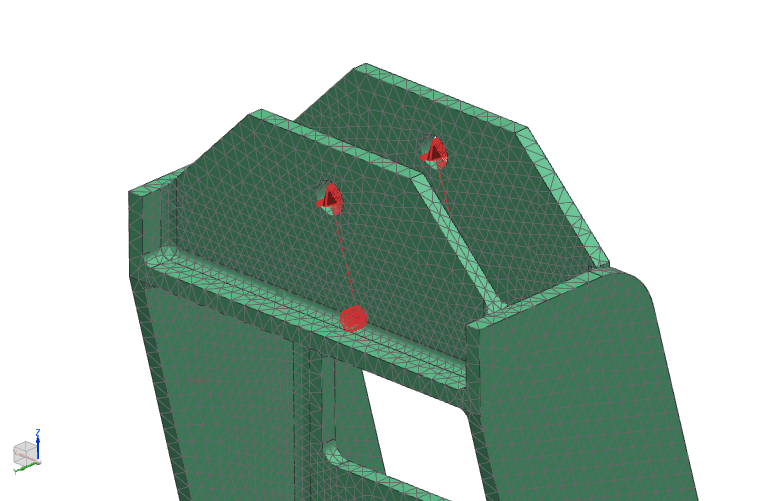
\includegraphics[width=2.5in]{images/Bilde_7.PNG} &
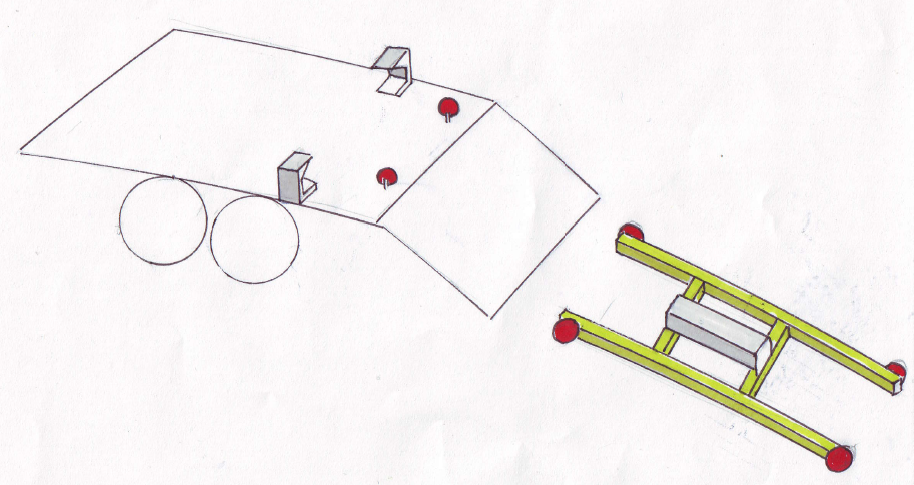
\includegraphics[width=2.5in]{images/Bilde_6.PNG} &  
\end{array}$
\end{center}
\caption{Krefter og grensebetingelser rammebrakett}
\end{figure}

Kjører simuleringen og får største spenning $\sigma_{max}$=31 MPa. Denne oppstår inne i hullene hvor hjulet på toppen er opplagret.

\begin{figure}[H]
\begin{center}$
\begin{array}{ccc}
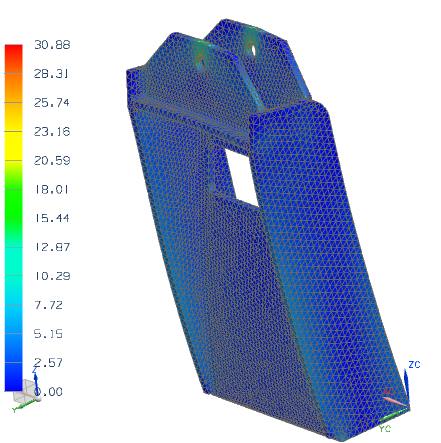
\includegraphics[width=2.0in]{images/Bilde_8.PNG} &
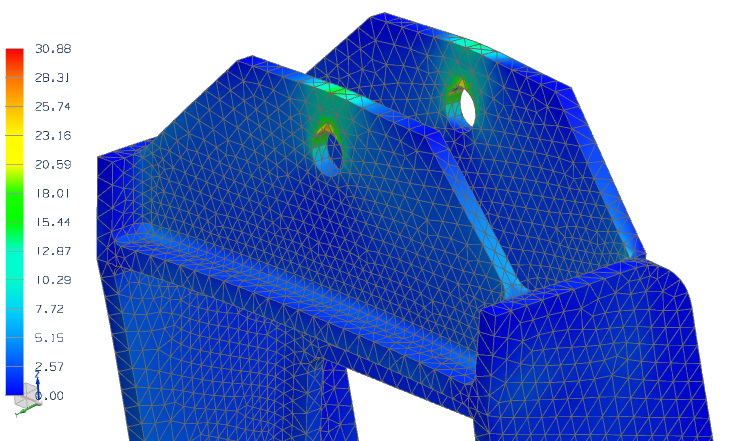
\includegraphics[width=3.0in]{images/Bilde_9.PNG} &  
\end{array}$
\end{center}
\caption{Von-Mises spenninger rammebrakett}
\end{figure}

Beregnet sikkerhet mot at det oppstår flyt i materialet:

\begin{equation}
\eta=\frac{225 MPa}{31 MPa}=7.25
\end{equation}\\

Rammebraketten vil ha en sikkerhet mot at det oppstår flyt i materialet på 7.25.\newpage

\subsection{Bein og Beinbrakett}
Setter på randbetingelser og krefter som vist nedenfor. I beinbrakettens hull påføres det en kraft tilsvarende bilens og rammens vekt i dette opplageret, F5=250N. Beinene må også sørge for å holde rammen stabil sideveis, samt framover og bakover. For å simulere dette påføres det krefter på F6=F7=100N nederst på beinet i x- og y-retning. Beinbraketten settes som fast låst på baksiden.

\begin{figure}[H]
\begin{center}$
\begin{array}{ccc}
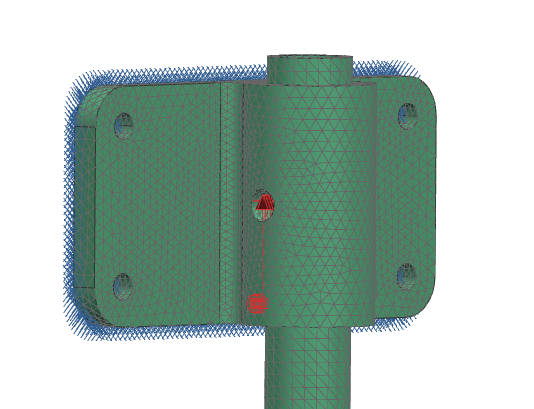
\includegraphics[width=2.5in]{images/Bilde_10.PNG} &
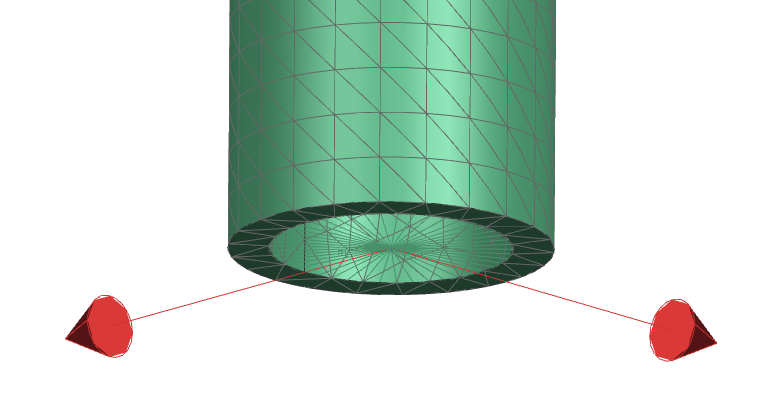
\includegraphics[width=2.5in]{images/Bilde_11.PNG} &  
\end{array}$
\end{center}
\caption{Krefter og grensebetingelser bein og beinbrakett}
\end{figure}

Kjører simuleringen og får største spenning $\sigma_{max}$=85 MPa. Denne oppstår nederst på innfestningen mellom beinbraketten og beinet.

\begin{figure}[H]
\begin{center}$
\begin{array}{ccc}
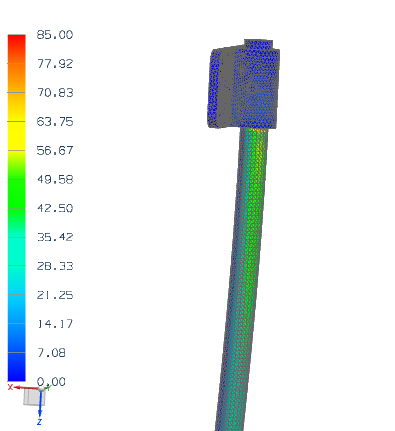
\includegraphics[width=2.0in]{images/Bilde_13.PNG} &
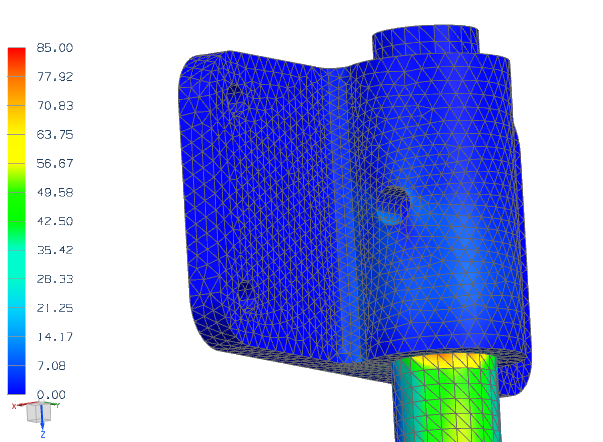
\includegraphics[width=3.0in]{images/Bilde_12.PNG} &  
\end{array}$
\end{center}
\caption{Von-Mises spenningerbein og beinbrakett}
\end{figure}

Beregnet sikkerhet mot at det oppstår flyt i materialet:

\begin{equation}
\eta=\frac{225 MPa}{85 MPa}=2.65
\end{equation}\\

Beinet og beinbraketten vil ha en sikkerhet mot at det oppstår flyt i materialet på 2.65.

\chapter{Brukergrensesnitt}
\section{Eksisterende system}
\subsection{Beskrivelse}

\paragraph{Brukergrensesnitt}
Brukergrensesnittet for å se status på bilen og løpet er ikke noe nytt system. 
Det ble laget et system av en tidligere EiT gruppe, dette systemet er laget ved hjelp av java og viser følgende data:
\begin{itemize}
\item Kart med bil
\item Hastighet
\item Grafer med måledata
\item Noen reléer
\end{itemize}
Et skjermbilde av dette er gjengitt i \ref{fig:gammeljava}.

\begin{figure}[H]
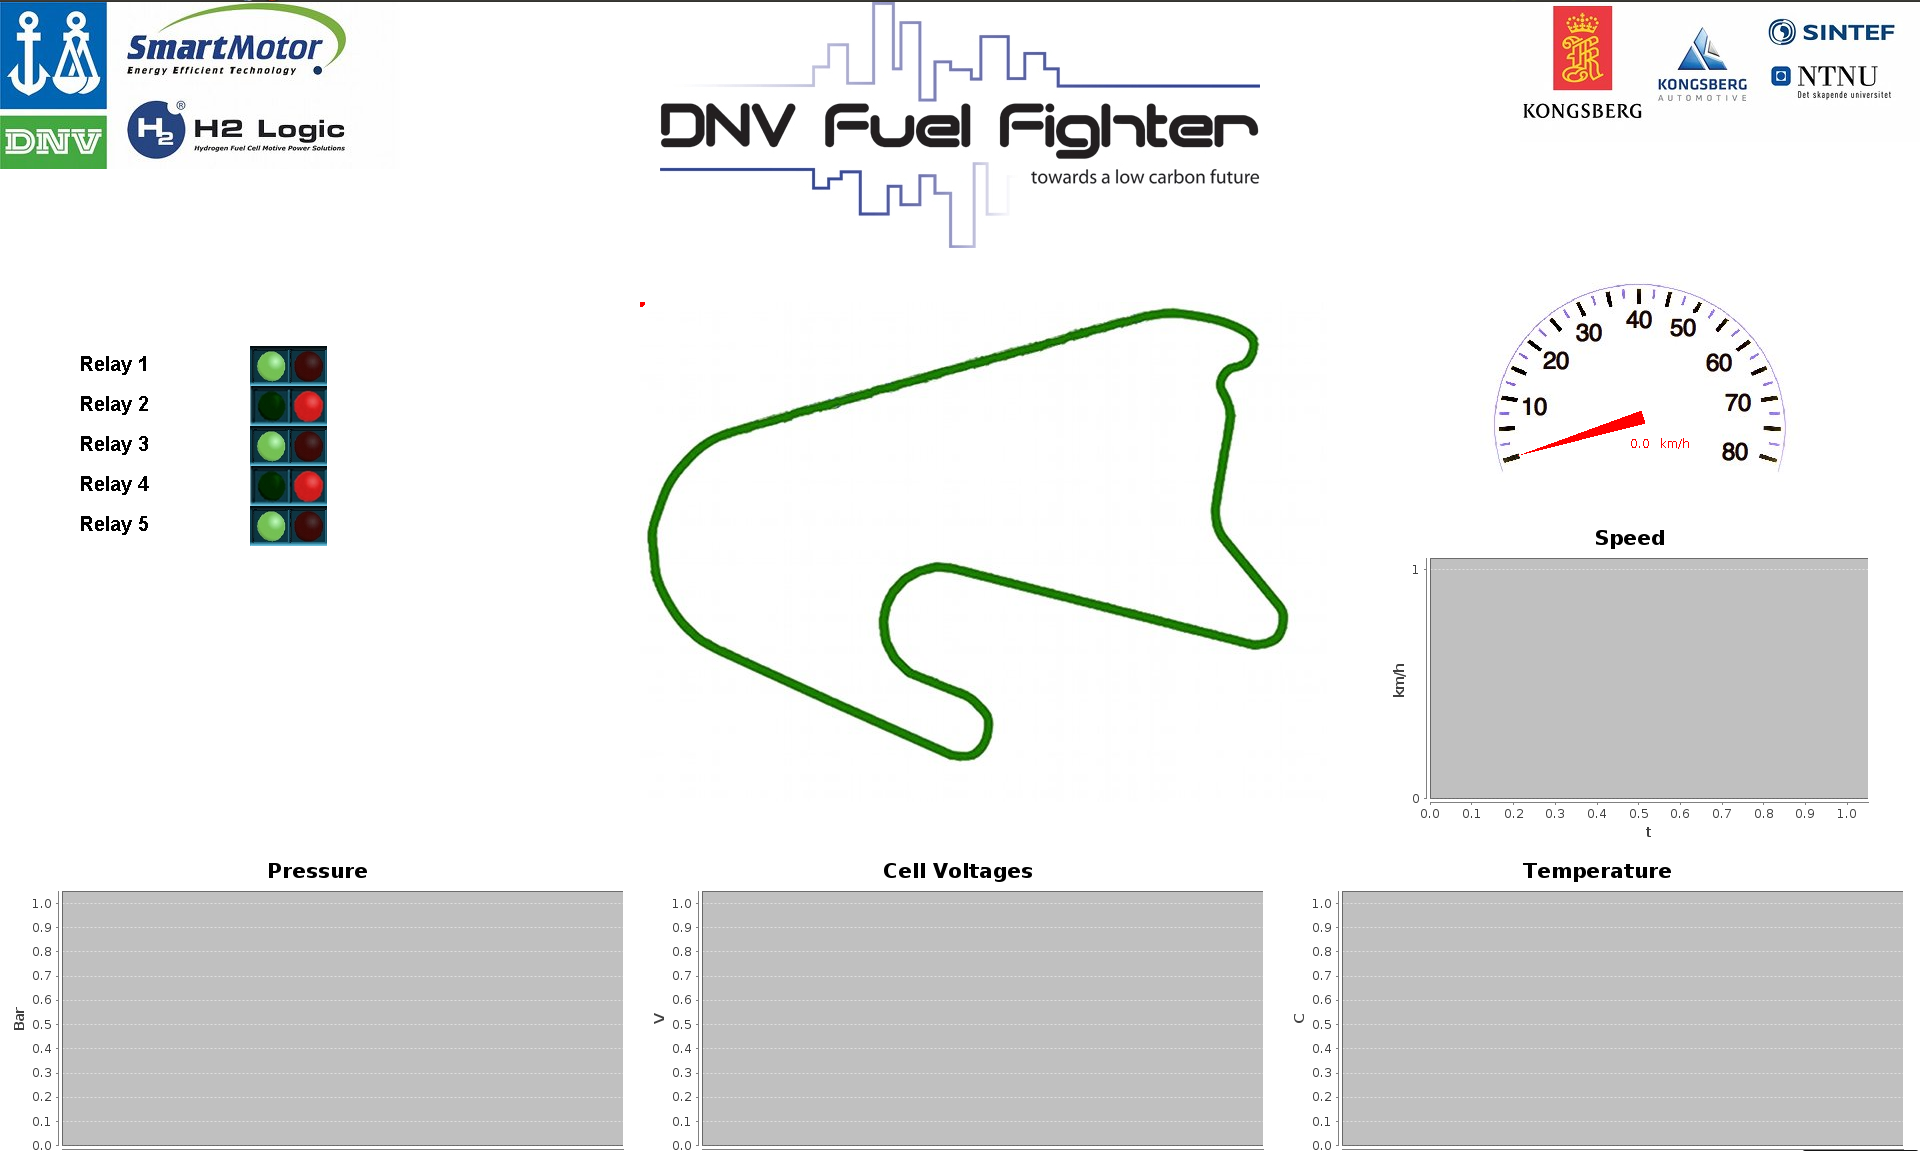
\includegraphics[width=\textwidth]{images/java.png}
\caption{Eksisterende system}
\label{fig:gammeljava}
\end{figure}

\paragraph{Telemetrimodul}
Modulen som sitter i bilen og sender data, ble laget av Anders Guldahl i 2009 \cite{telemetrithesis}, denne leser forskjellige parametre fra resten av bilen, og sender dette over GPRS til en server.

\subsection{Problemer og ulemper}
\paragraph{Brukergrensesnitt}
Det ble funnet noen problemer ved det eksisterende systemet:
\begin{itemize}
\item Har ikke mulighet til å vise kart for hvor bilen er annet enn på banen.
\item Kan ikke vise historie på måledata.
\item Kun for bruk internt med Ecomarathon, kan ikke brukes f.eks. i PR sammenheng på nett.
\item Fungerte ikke under selve løpet. Det mistenkes at dette skyldtes bilen og ikke systemet, men ingen vet sikkert.
\item Ingen på prosjektet vet hvordan det brukes.
\end{itemize}
I tillegg til dette kom det ønsker om hvordan det skal se ut fra resten av Ecomarathon teamet, noe som er vanskelig å endre i det eksisterende systemet.

\paragraph{Telemetrimodul}
Telemetrimodulen har noen svakheter som må løses før den fungerer slik den skal.
Ved konkurransen i fjor sendte ikke bilen data når den var i Tyskland.
Telemtrimodulen har heller ikke implementert at den skal sende data om posisjon og hastighet.


\section{Initieringsfase}
\section{Konsepter}
Etter at det ble klart hva gruppa skulle gjøre, gjennomførte vi en brainstorm om hvordan brukergrensesnittet skulle se ut.
Alle på gruppa forsøkte å tegne konsepter på grensesnittet, og her er noen av ideene som ble brukt i konseptene:

\paragraph{Kart}
Oppgaven går ut på å vise data fra telemetrimodulen på bilen, og siden denne er utstyrt men en gps, er det en mulighet å vise posisjonen til bilen på et kart.

\paragraph{Riktig fart}
Ideen var et speedometer som ikke viste hastiget, men hastighet relativt til optimal hastighet. 
Siden bilen bruker mindre energi ved lavere hastighet, ønsker man å holde en så lav hastighet som mulig, men fullføre løpet innen gitt tid.
Et slikt speedometer vil da vise hvor mye man bør øke eller senke hastigheten for å komme i mål akkurat tidsnok.

\paragraph{Tid og splittid}
Konseptet bestod av en tabell med rundetider og splittider.
Splittidene listes opp horisontalt for hver runde, og rundene listes opp vertikalt.
Tidene skal kunne vises enten som brukt tid, eller differansen mellom planlagt og brukt tid.
Dette gjør det lett å sammenligne de ulike rundene, og planlegge ulike hastigheter for disse.

\paragraph{Trending av måledata}
Siden måledata hele tiden endrer seg, vil det være interessant å se hvordan dataene har endret seg over tid.

\paragraph{Bruk av farger}
Å benytte farger til måledata vil kunne gjøre det enklere for en bruker å vite betydningen av en måleverdi.

\paragraph{Skjuling av måleverdier}
Siden måledata er mest interessante når de ikke er innen normale verdier, kan disse skjules når de normale.
Dette vil gi brukeren mindre data å holde orden på.

\section{Vurdering}
For å vurdere disse konseptene valgte vi å ta et møte med ecomarathon teamet, siden vi manglet grunnlag for å sette opp en vurderingsmatrise. 
Vi snakket først med Jardar, og tegningen til Hans falt i god smak. 
Det ble klart at tid var langt mer viktig enn fart, så hovedskjermbildet ble det avgjort skulle først og fremst inneholde rundetider og et kart over banen. 
Trending av data ble det klart burde kombineres med å holde disse skjult når disse ikke var interessante.
Ideen om å vise splittider ble etter hvert avvist av Uwe, som mente disse ville bli vanskelige å implementere. 
Et av problemene er at man ikke har nøyaktige avstander på banen, men også at man er nødt til å stoppe en gang for hver runde.


\section{Løsningen}
\subsection{Dataflyt fra bilen til brukergrensesnitt}
Hele løsningen rundt å få data fra bilens telemetrimodul til brukeren er realisert med 3 modulerer som gjør hver sin jobb for å frakte dataene.
\begin{figure}[H]
\caption{Dataflyt} 
\label{dataflow}
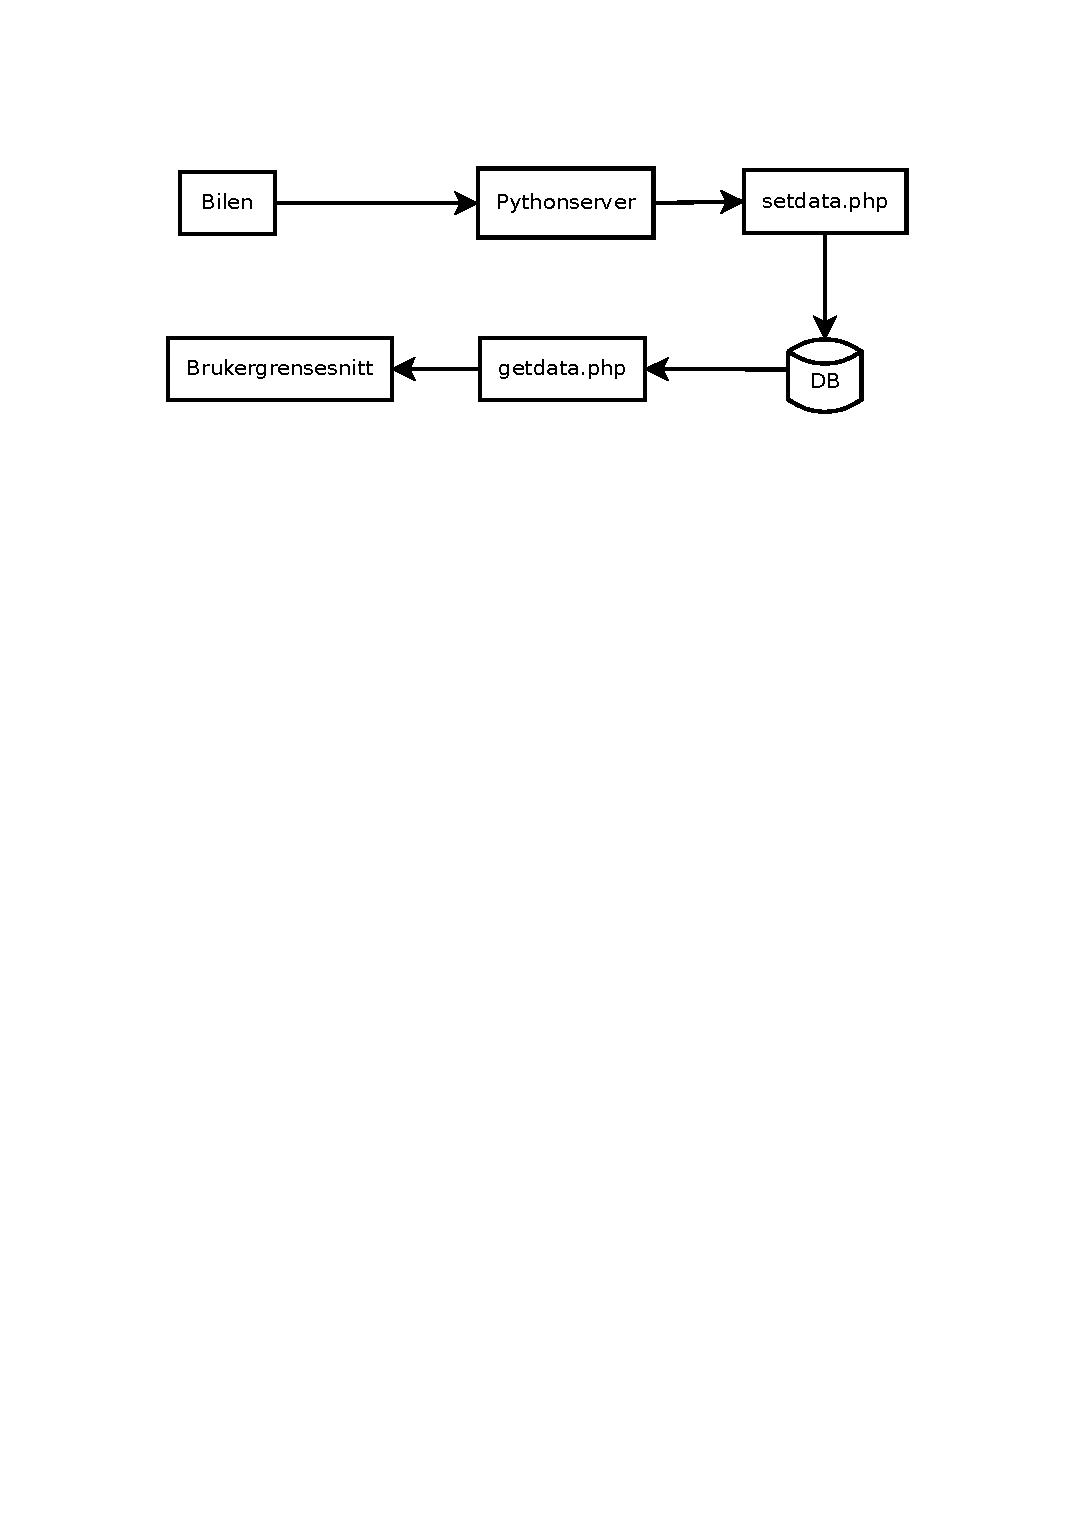
\includegraphics[width=\textwidth, trim=0 550 0 75]{images/dataflow.pdf}
\end{figure}
\subsubsection{Databasen}
Databasen som kjører bak alt er en enkel MySQL-database, denne holder historikk på sensorer, tider og andre data som må være persistente. Et ER diagram over databasen kan sees i \ref{er}, her er config spesiell, dette er en tabell som bare har en rad fordi den skal holde globale variable for hvorvidt løpet er startet og hvor de andre dataene kan hentes fra.
\begin{figure}[H]
\caption{Databasen} 
\label{er}
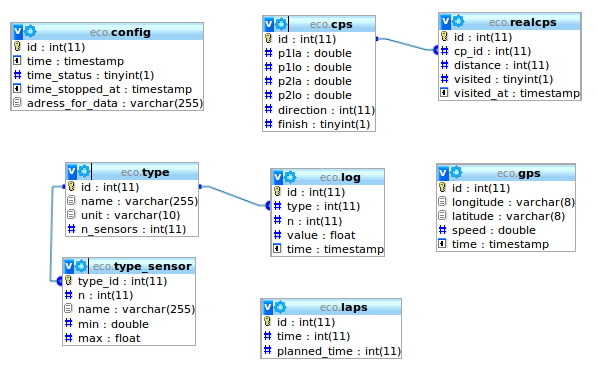
\includegraphics[width=\textwidth]{images/er.png}
\end{figure}

\subsubsection{Pythonserver}
Pythonserver er et lite script skrevet i Python som setter opp en TCP socket for å motta data som telemetrimodulen sender. Så fort den har mottatt en hel pakke med data fra bilens telemetrimodul gjør den en omregning av gpsposisjonene fra grader og minutter til rene grader på decimalformat. Deretter sender den dette videre ved å sette opp en HTTP connection til webserveren og sender dataene som et POST request til setdata.php.
\subsubsection{setdata.php}
Denne modulen tar i mot kommaseparerte data fra Pythonserveren og setter disse inn i databasen. I tillegg gjør den utregninger i forhold til om bilen har passert kontrollpunkt og oppdaterer tidstabellen i henhold til dette hvis løpet er startet fra brukergrensesnittet.
\subsubsection{getdata.php}
Denne brukes for å hente data fra databasen når websiden vises. Den slår opp i databasen og bygger opp et script med jQuery\cite{jquery} som igjen oppdaterer elementer i guiet.
\subsection{Brukergrensesnitt}
Brukergrensesnittet er bygget uten hjelp av noe spesielt rammeverk, men i stedet bygget fra grunnen ved hjelp av PHP, javascript og jQuery\cite{jquery}. Det kjører en jqueryfunksjon som hver x. minutt henter et nytt script som getdata.php genererer og oppdaterer elementene i brukergrensesnittet med det. Brukergrensesnittet har et kart som bruker api fra google for å sette logoen til fuelfighter på kartet og få den til å bevege seg utifra data fra bilen. Hastigheten til bilen blir gjengitt ved hjelp av et speedometer fra Bindows Gauges\cite{bindows}. En oversikt over hvordan det ferdige systemet ser ut kan sees in en skjermdumpen \ref{gui}. Stoppeklokken som sees på toppen her drives av et lite javascript. Ved å klikke på Start så settes et tidspunkt i databasen og klokka begynner å gå, dette tidspunktet brukes så av setdata.php for å regne ut rundetider på banen. Hvis det trykkes på Stop så stoppes klokka slik at brukeren kan stoppe løpet ved uforutsette hendelser i løpet.
\begin{figure}[H]
\caption{Ferdig system} 
\label{gui}
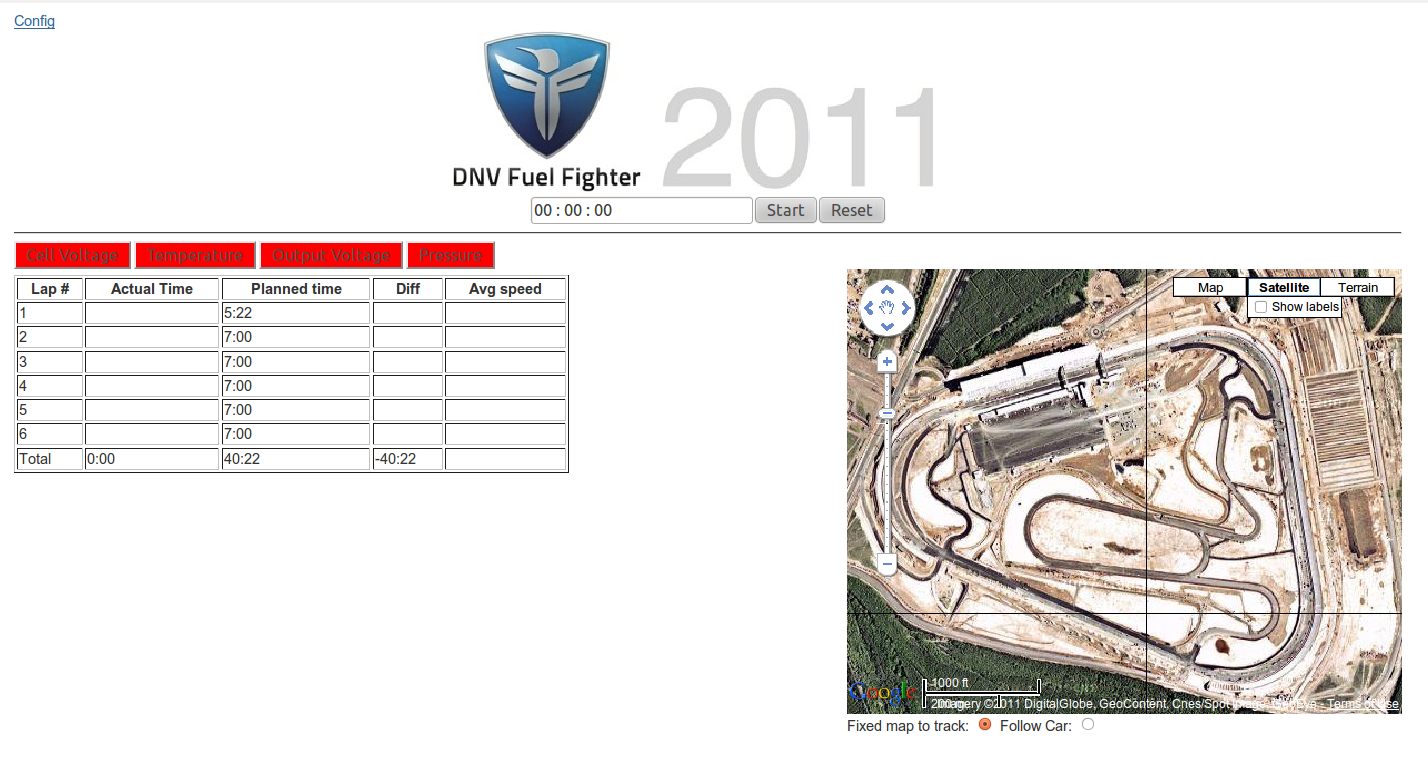
\includegraphics[width=\textwidth]{images/gui.png}
\end{figure}
\subsubsection{Konfigurasjon}
Det finnes også et brukergrensesnitt for at brukeren av systemet skal kunne sette navn, måleenhet og grenseverdi på sensorer. I tillegg kan også planlagte tider og hvor dataene skal hentes fra settes her.
En skjermdump av dette finnes i \ref{config}, dette kommer opp som et vindu over grensesnittet i \ref{gui}.
\begin{figure}[H]
\caption{Config} 
\label{config}
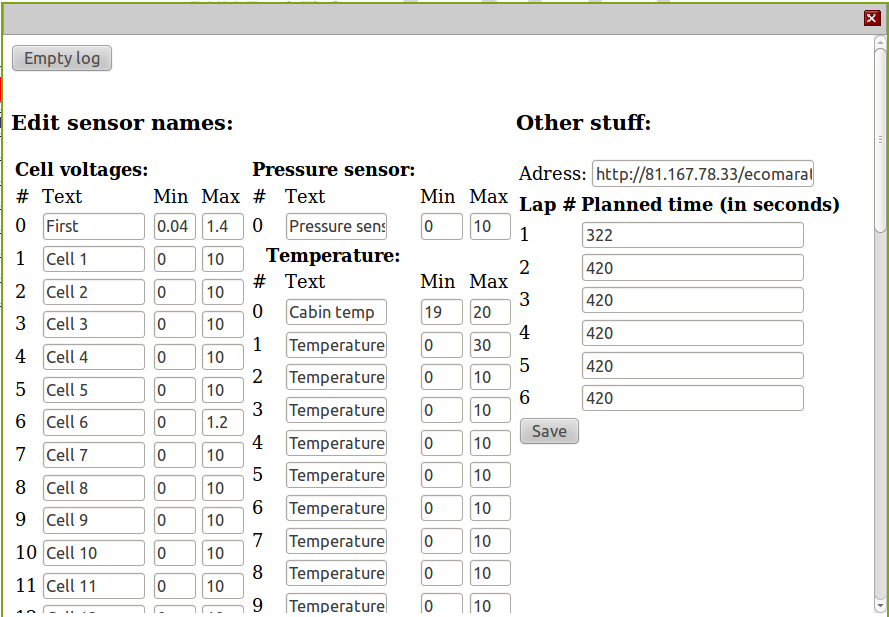
\includegraphics[width=200px]{images/config.png}
\end{figure}

\subsubsection{Statistikk}
Hver sensor kan trykkes på og da kommer vinduet som er vist i \ref{stats} opp, dette genereres ut i fra det som blir lagt inn av databasen. Her kan man navigere frem og tilbake i historien for å finne ut når en sensor har meldt om feil. Grafen tegnes opp ved hjelp av biblioteket highcharts \cite{highcharts}.
\begin{figure}[H]
\caption{Statistikk} 
\label{stats}
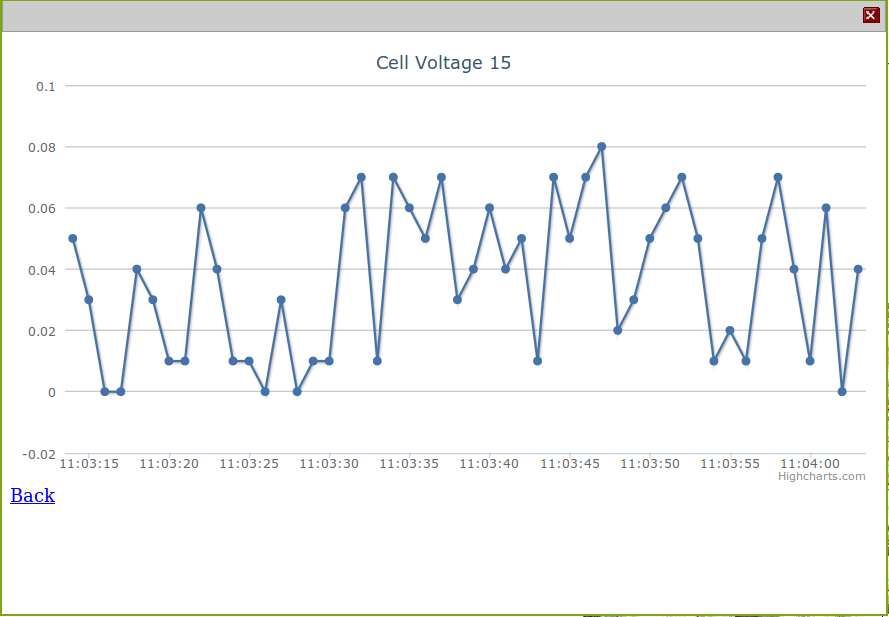
\includegraphics[width=200px]{images/stat.png}
\end{figure}
\subsection{Telemetrimodul}
Telemtrimodulen ble laget av Anders Guldahl \cite{telemetrithesis} i 2009. Denne har ikke blitt endret mye på, men noen endringer måtte gjøres for at den skulle fungere sammen med brukergrensesnittet.
Slik det var, så leverte telemetrimodulen GPS data kun til dashbordet i bilen og hastigheten til bilen ble aldri brukt. Dette er nå endret slik at telemetrimodulen sender disse dataene sammen med de andre måleverdiene som en komma separert string via GPRS til Pythonserveren.


\appendix
\chapter{Arbeidstegninger}
\newpage
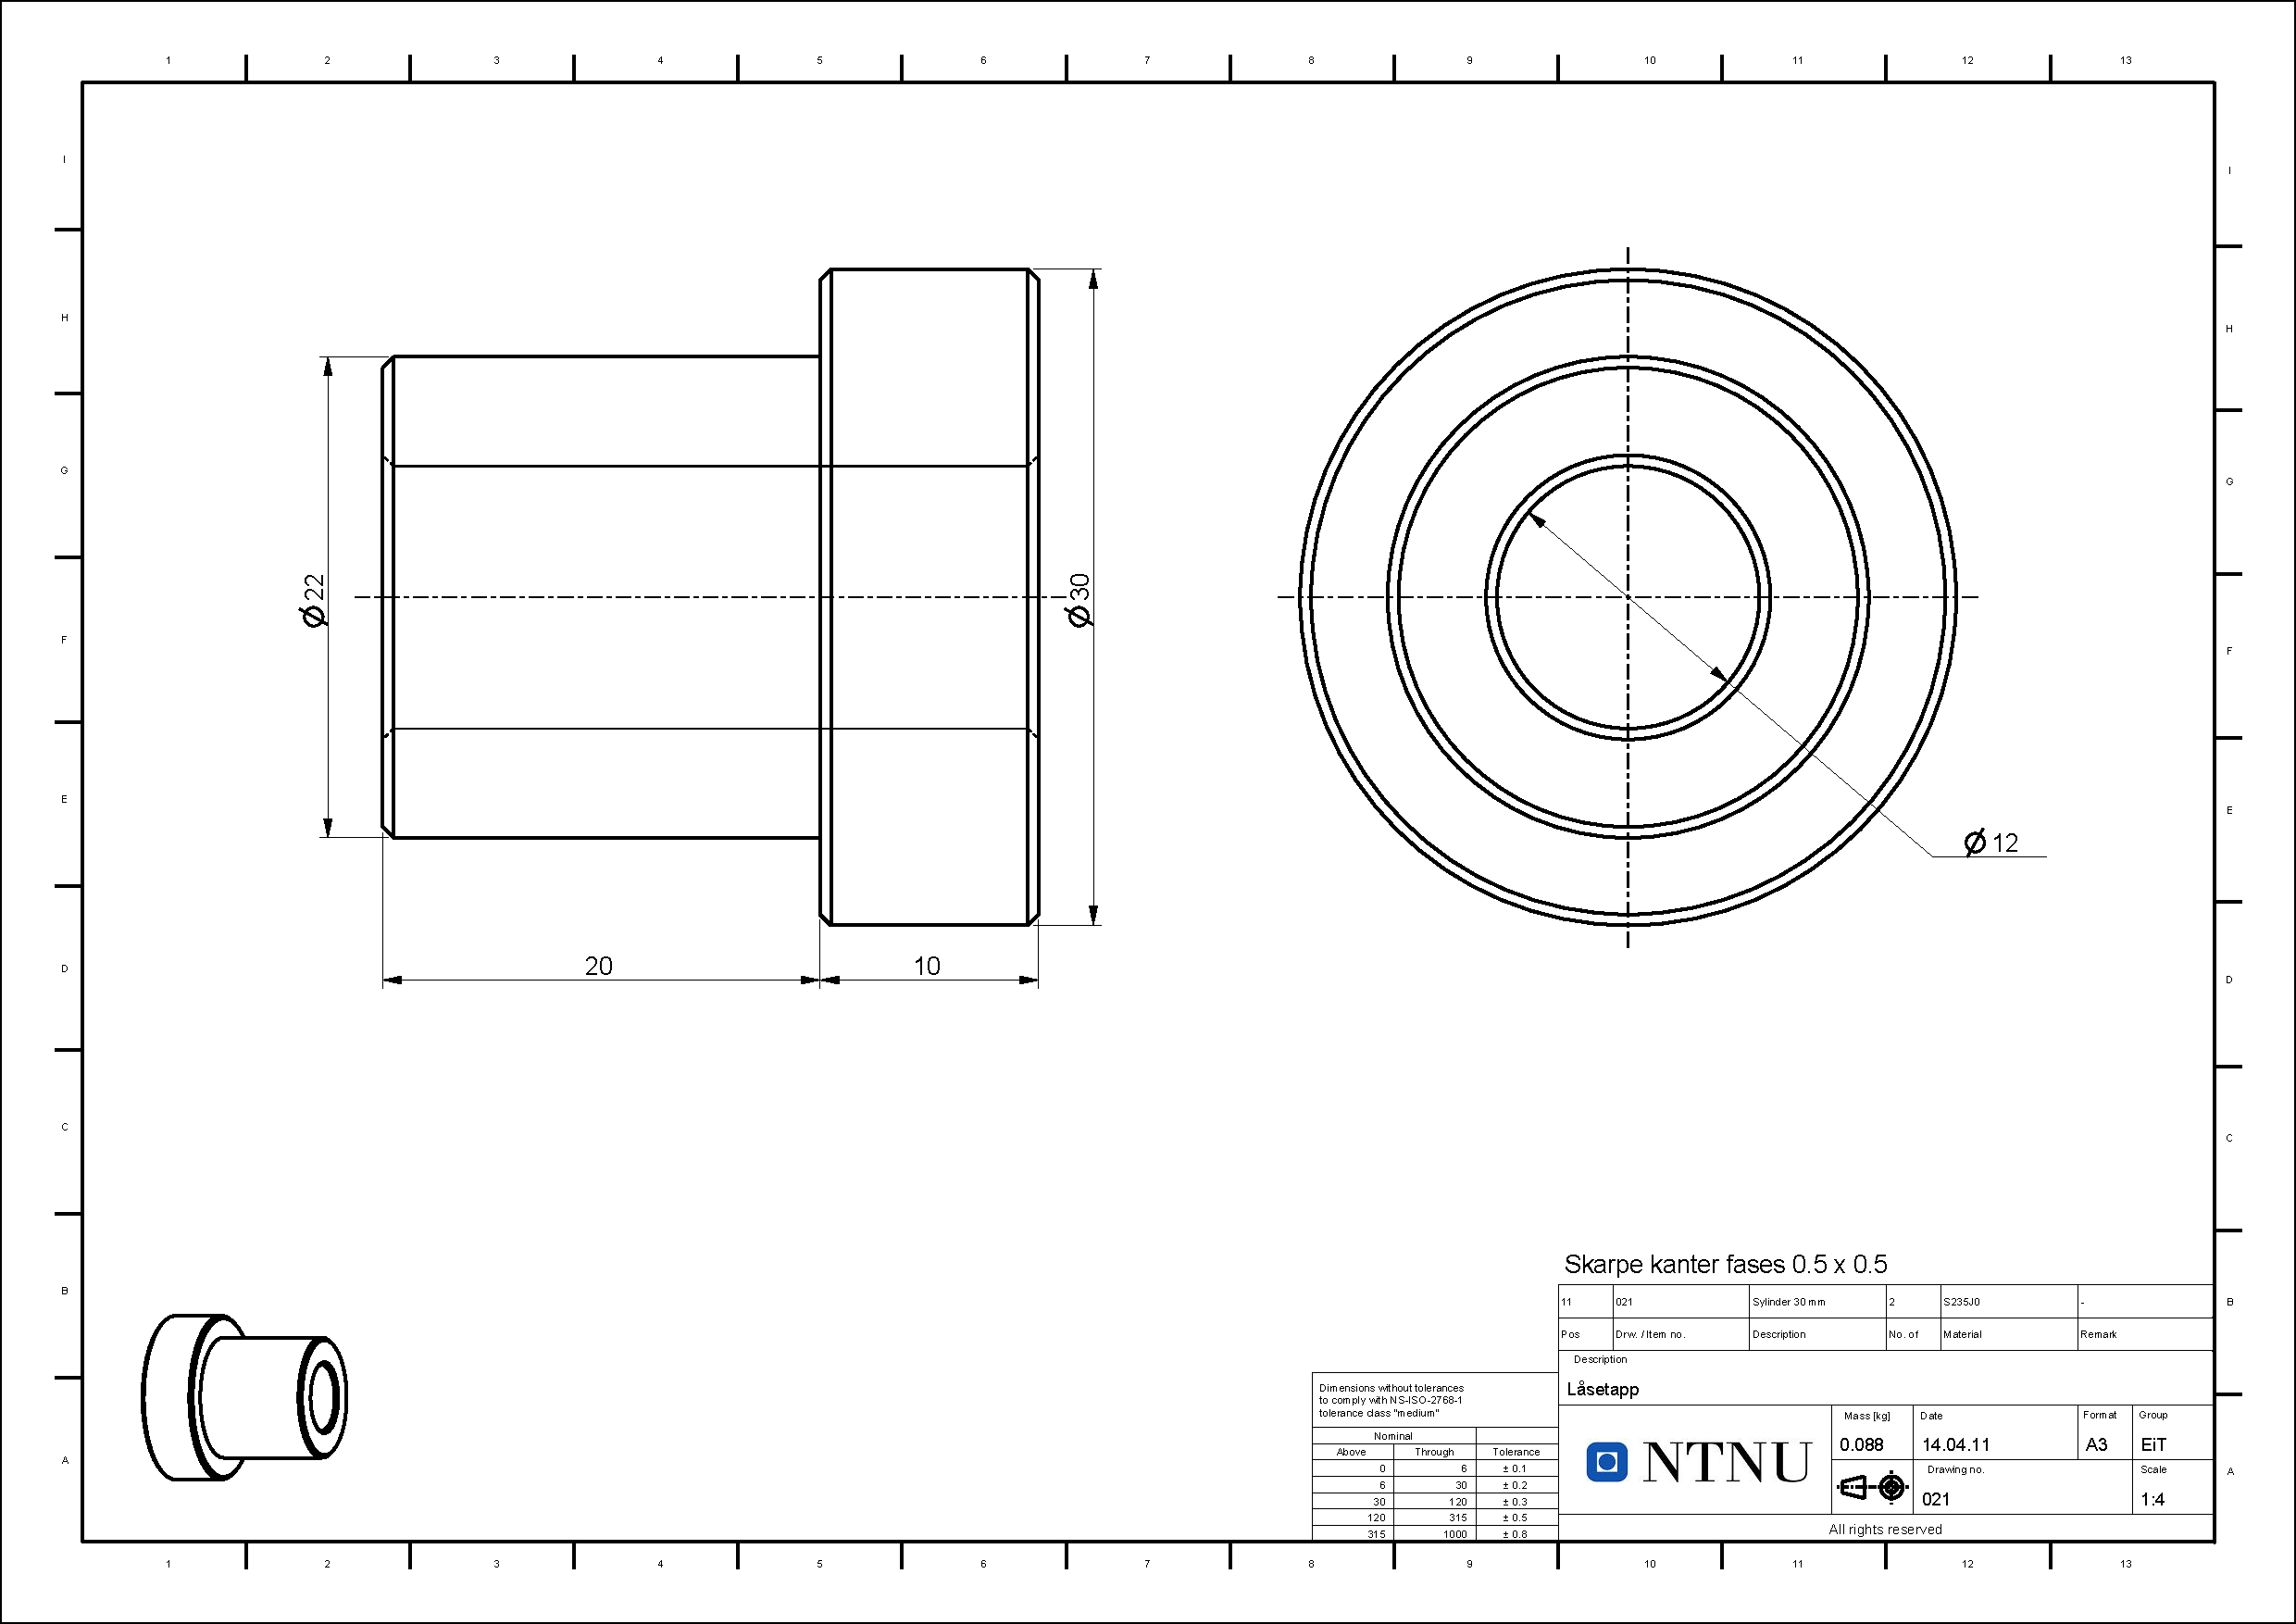
\includegraphics[angle=90, width=\textwidth]{arbeidstegninger/021}\newpage
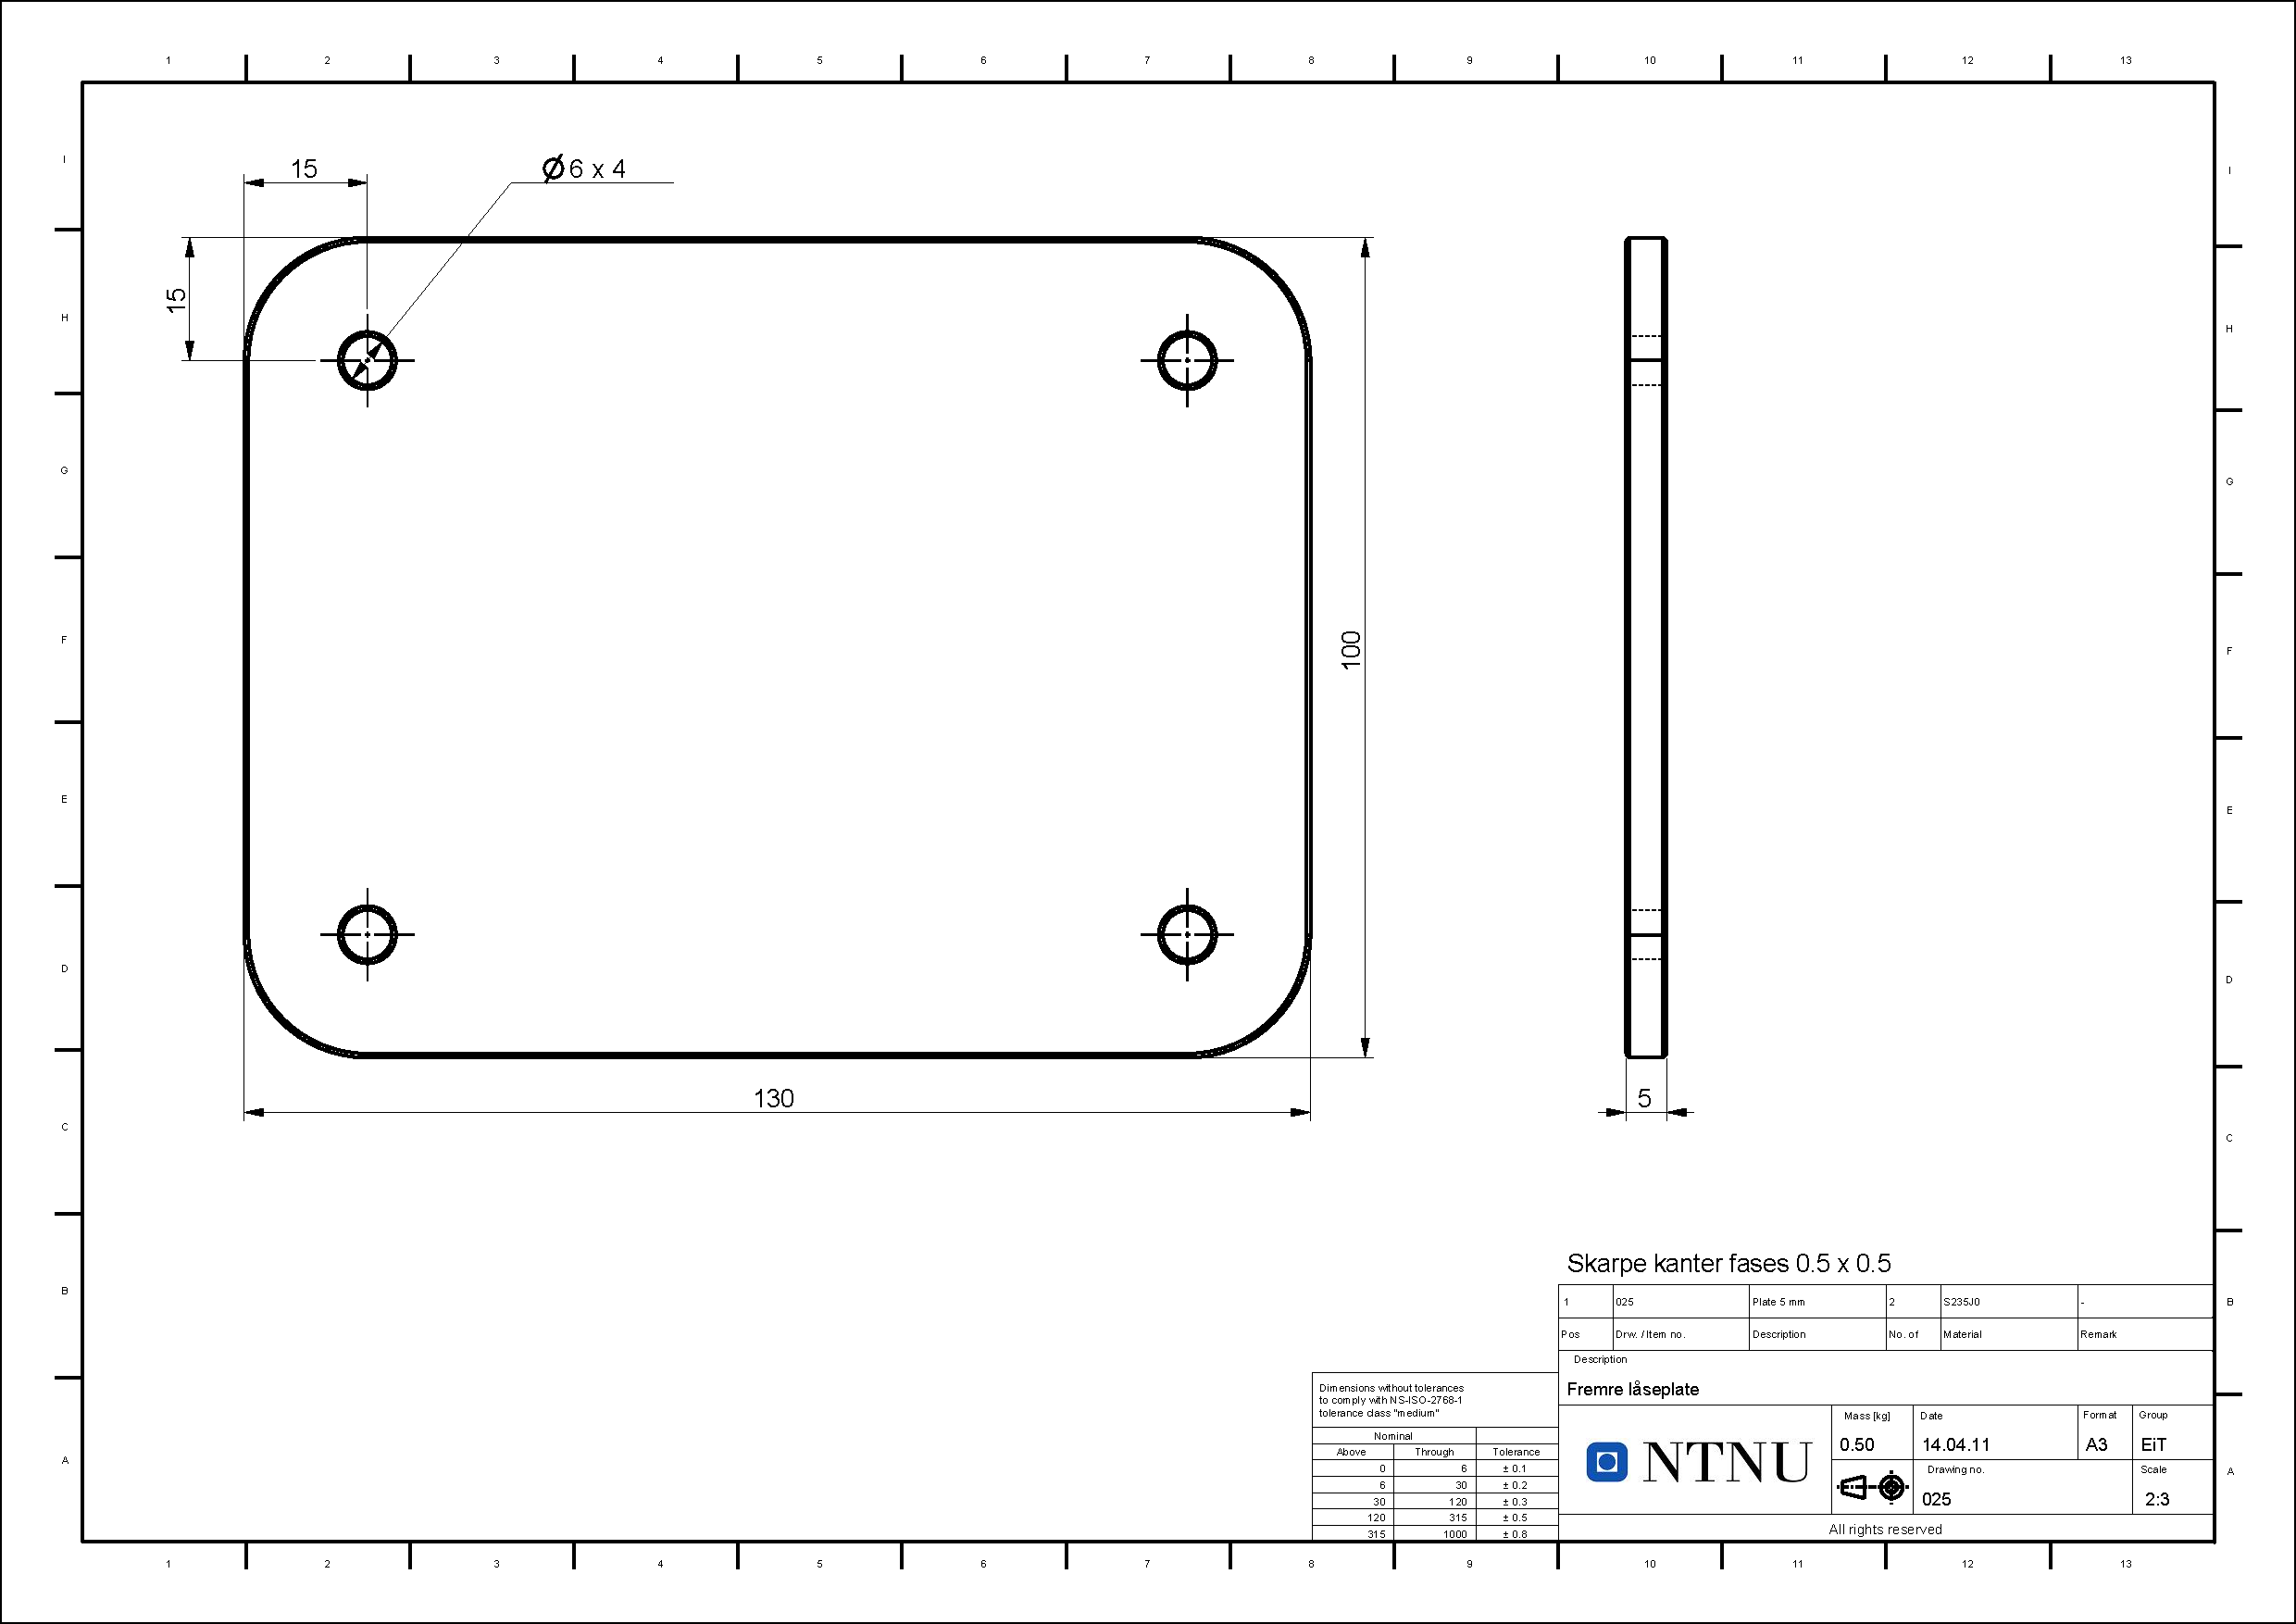
\includegraphics[angle=90, width=\textwidth]{arbeidstegninger/025}\newpage
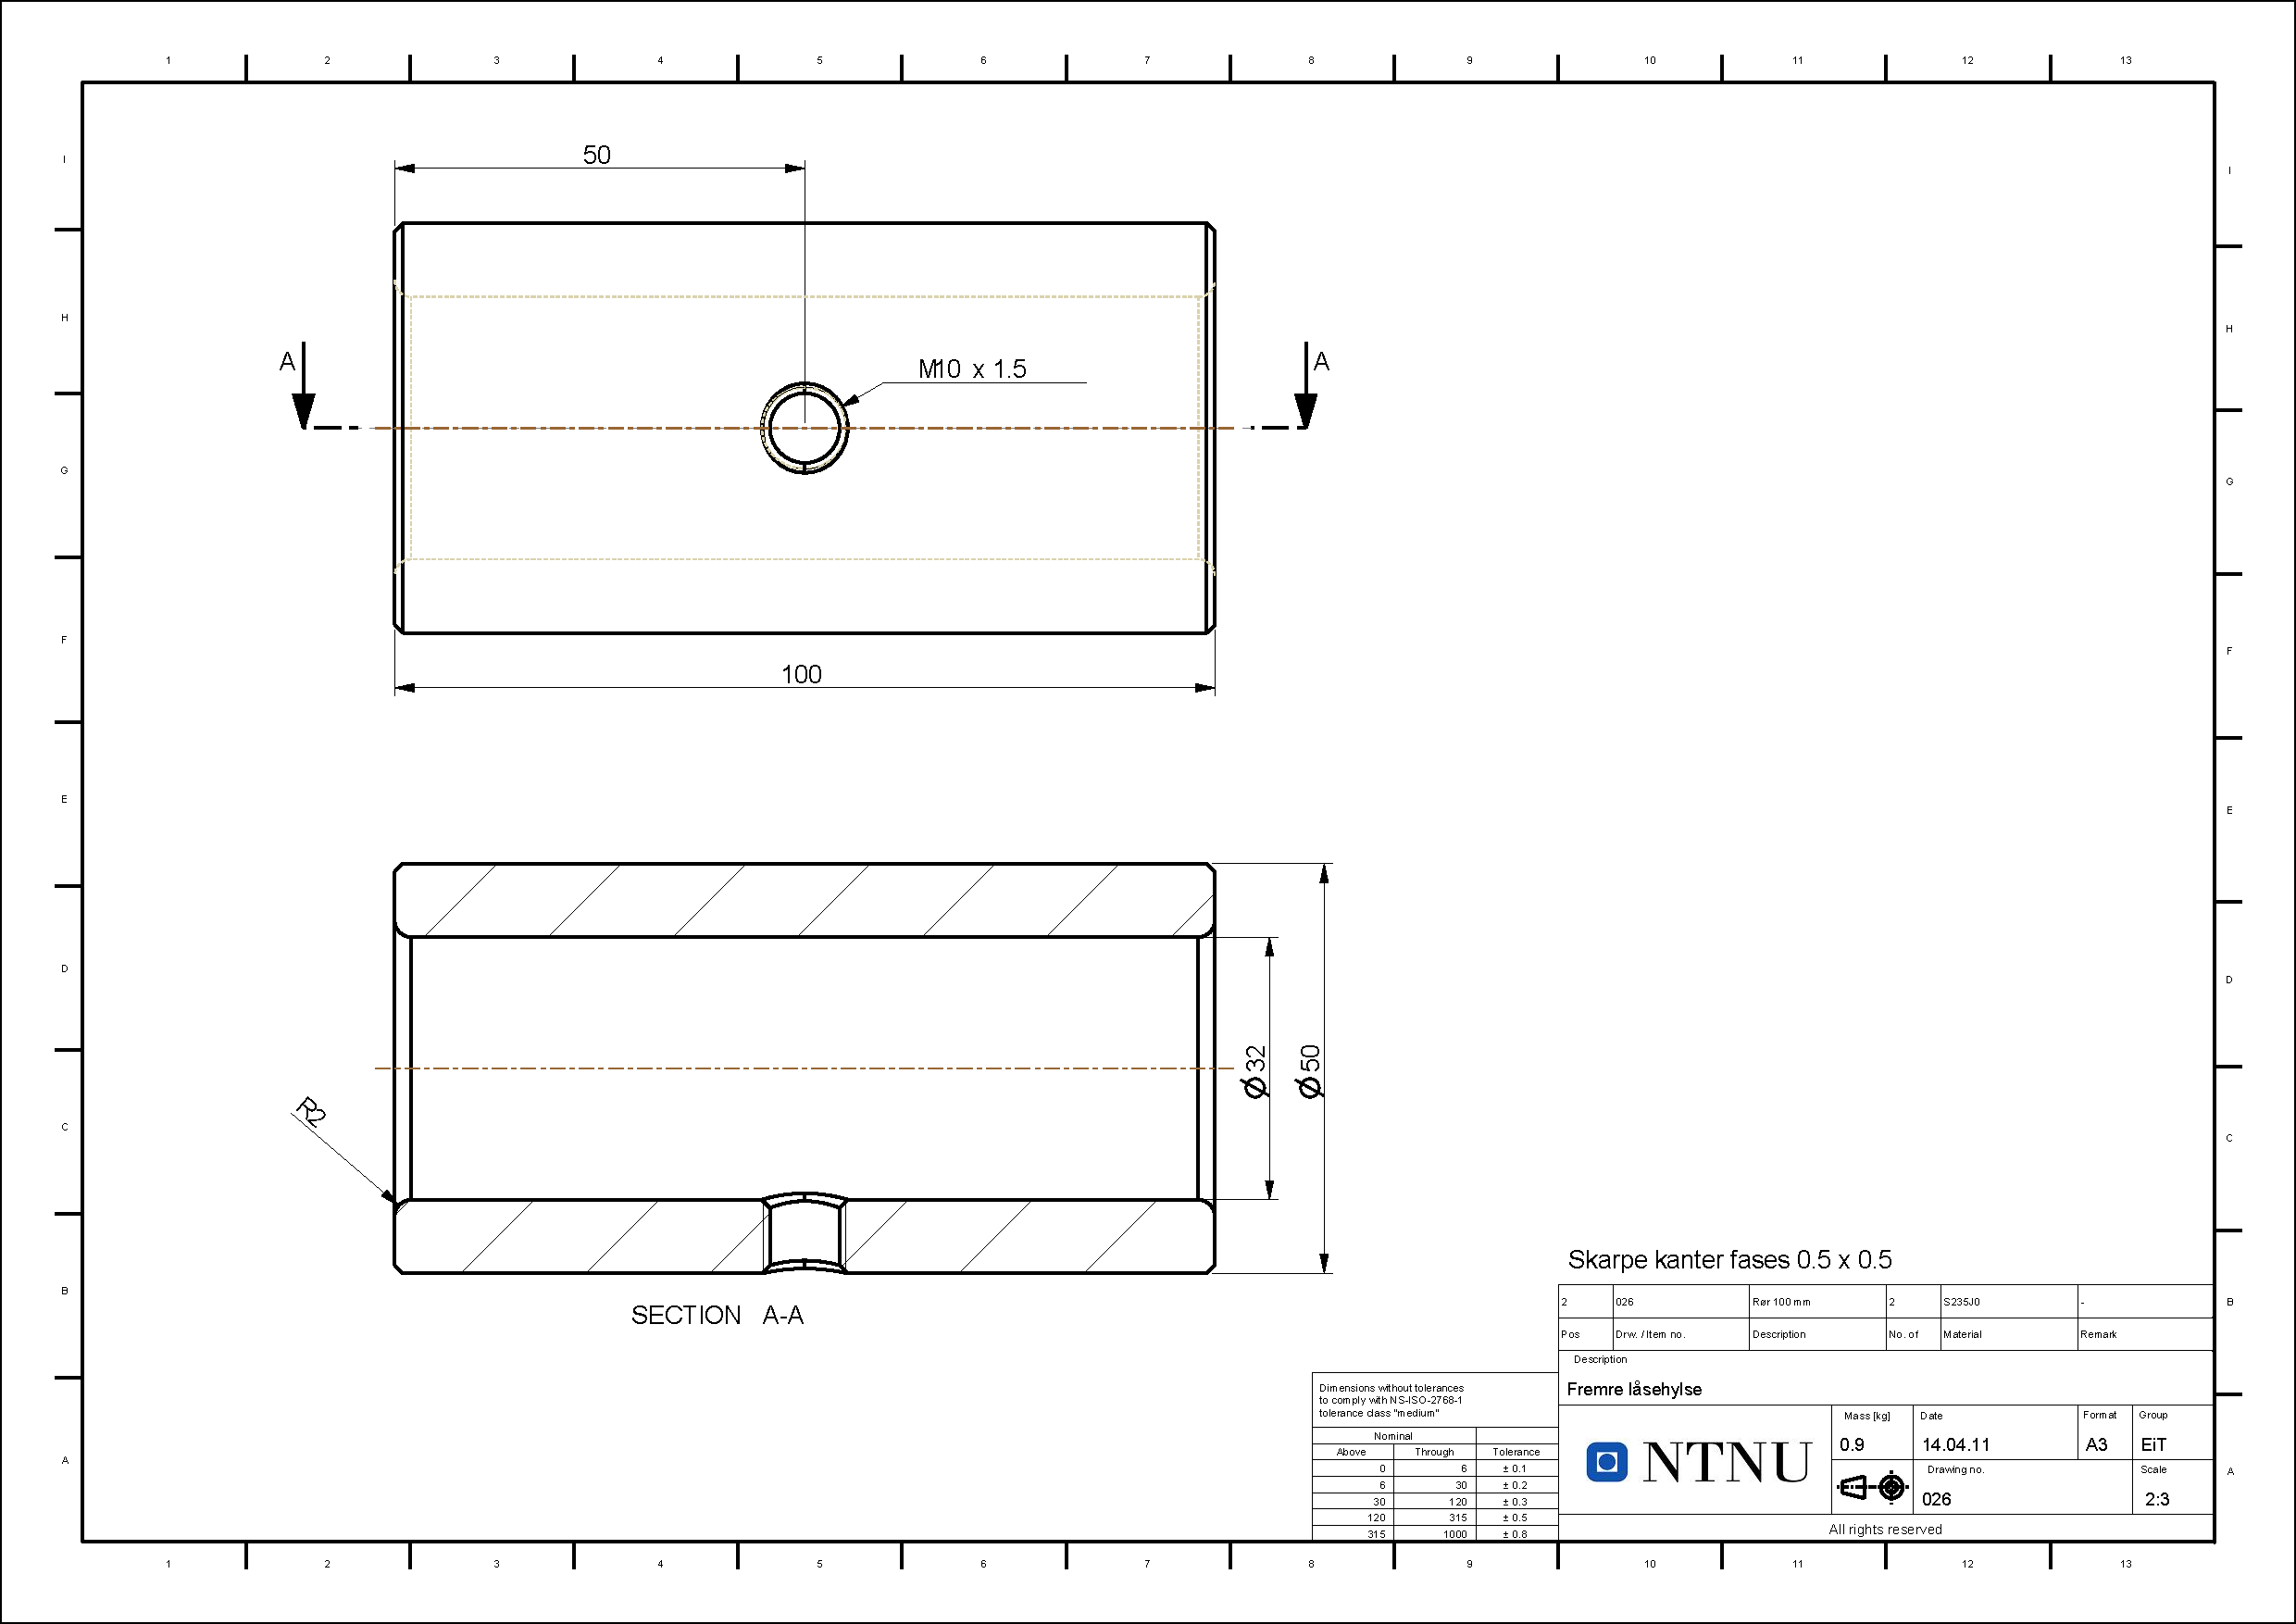
\includegraphics[angle=90, width=\textwidth]{arbeidstegninger/026}\newpage
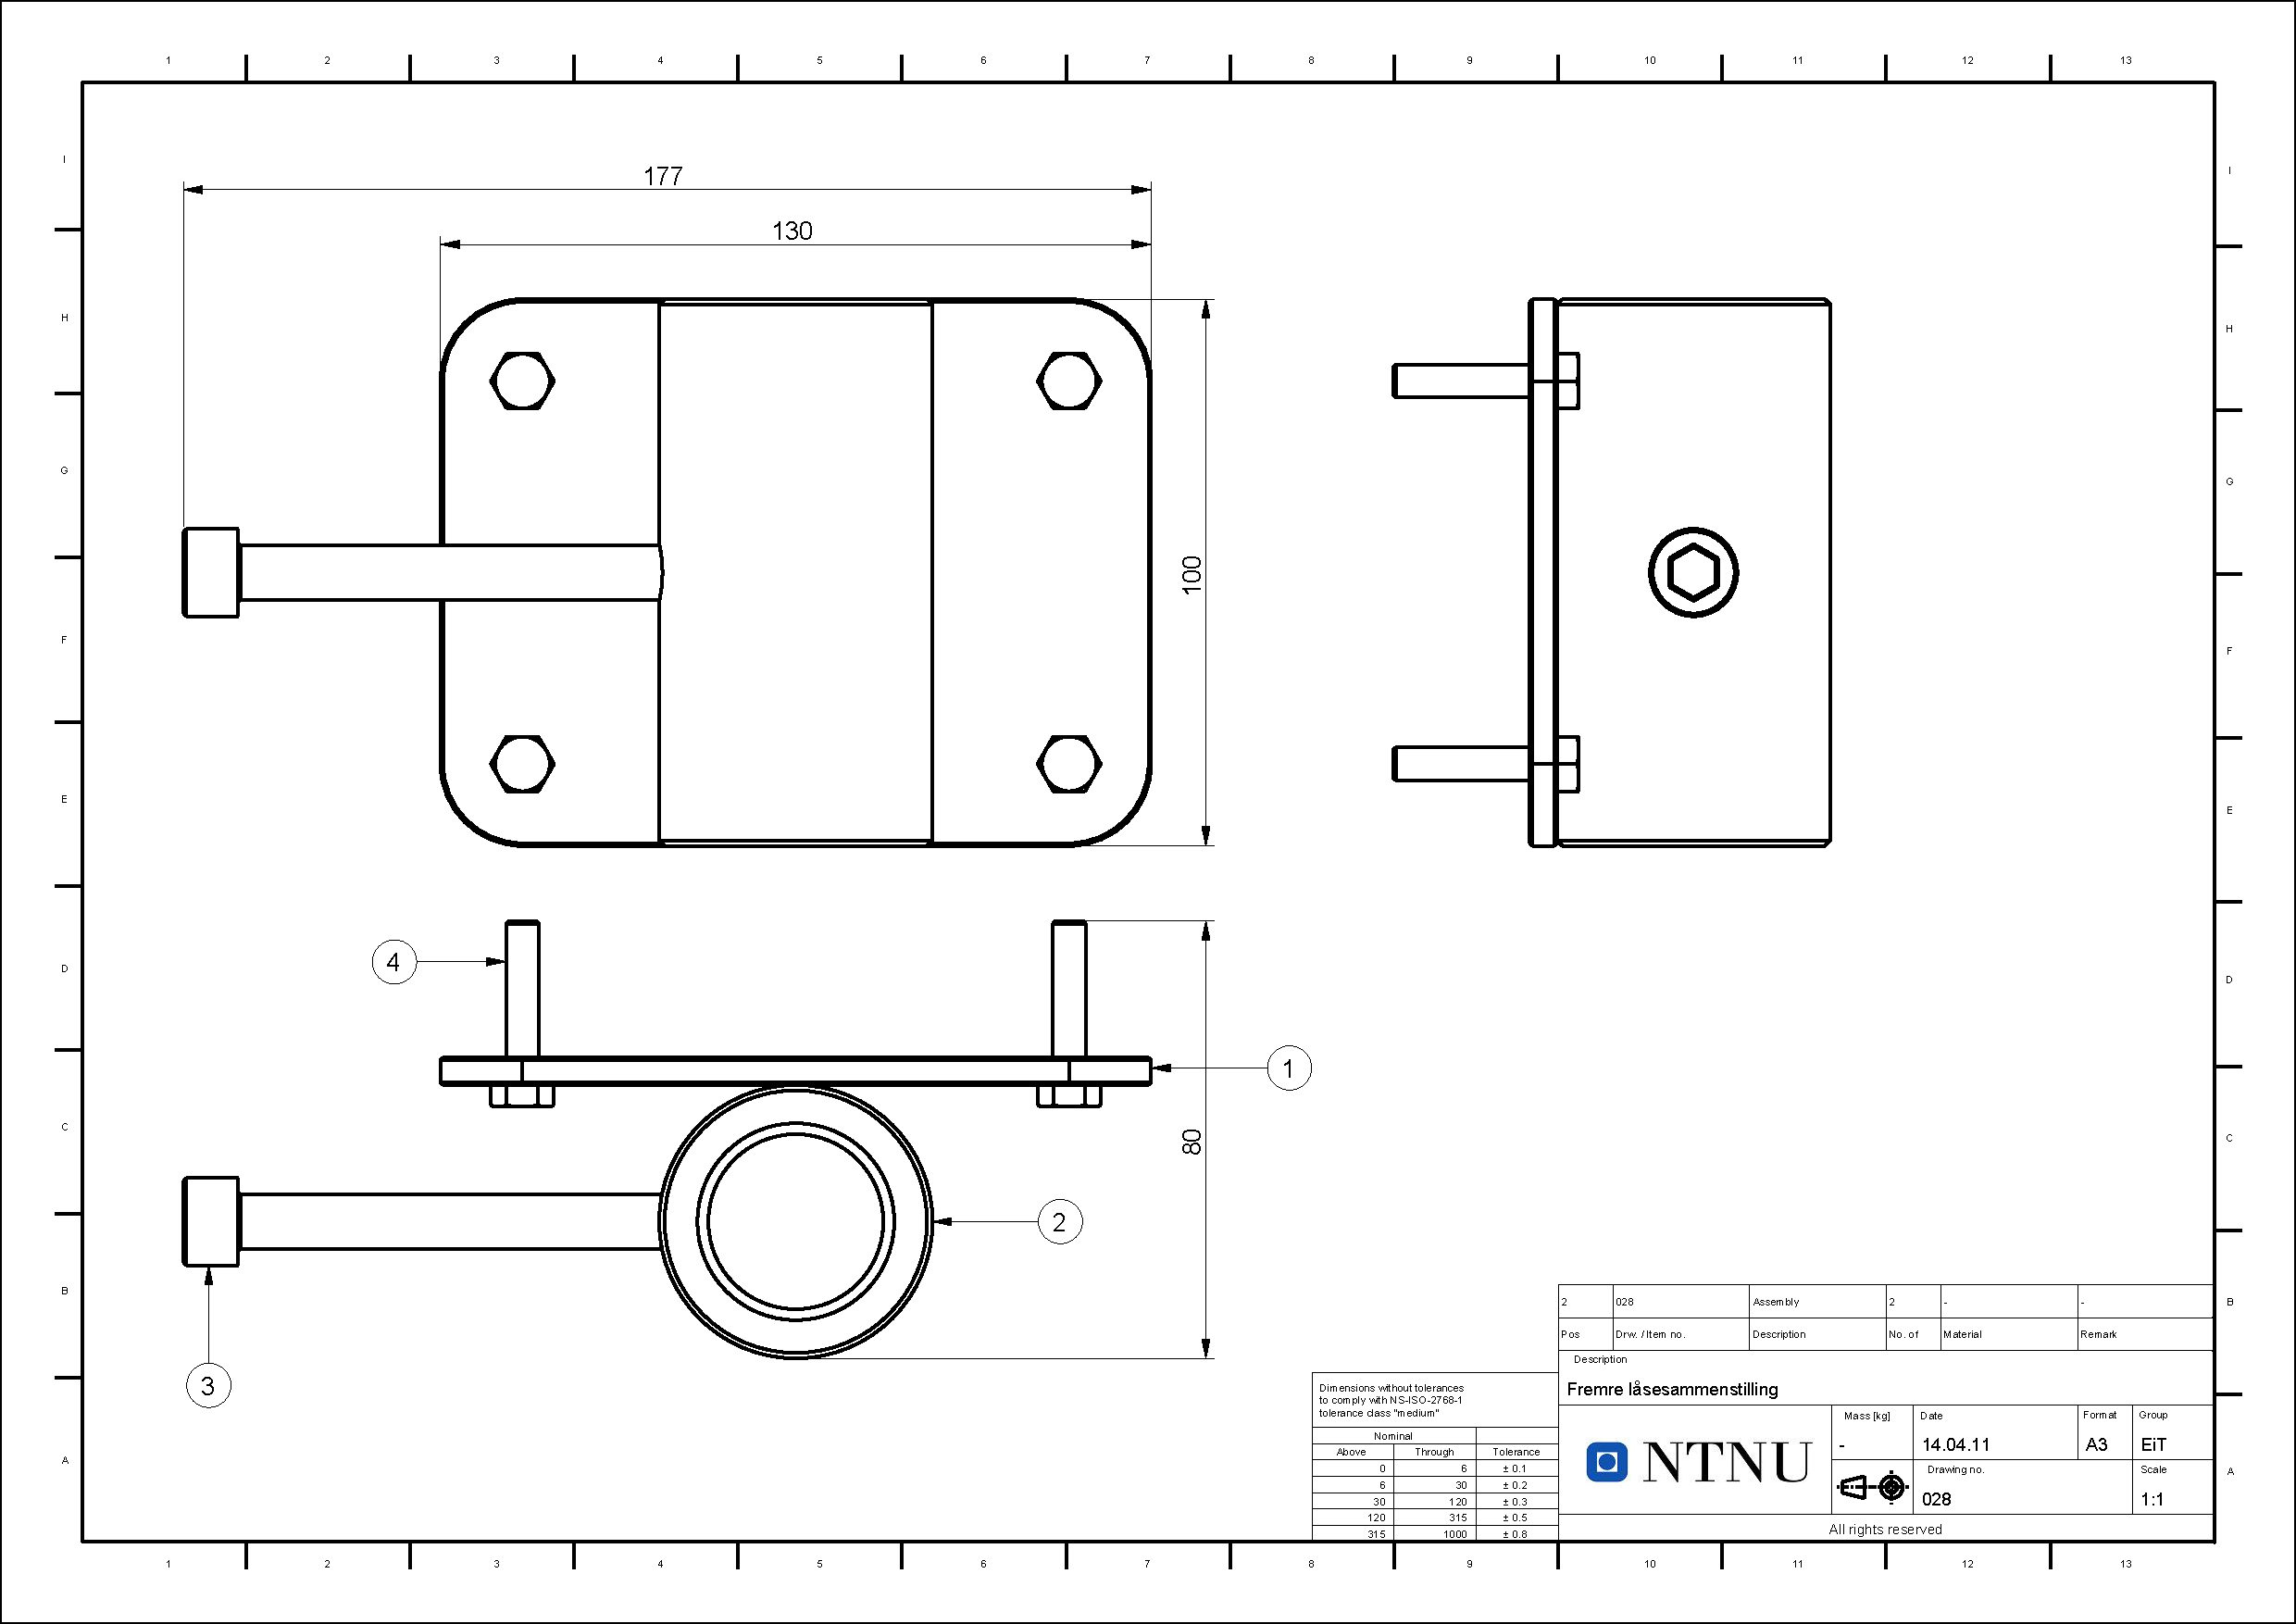
\includegraphics[angle=90, width=\textwidth]{arbeidstegninger/028}\newpage
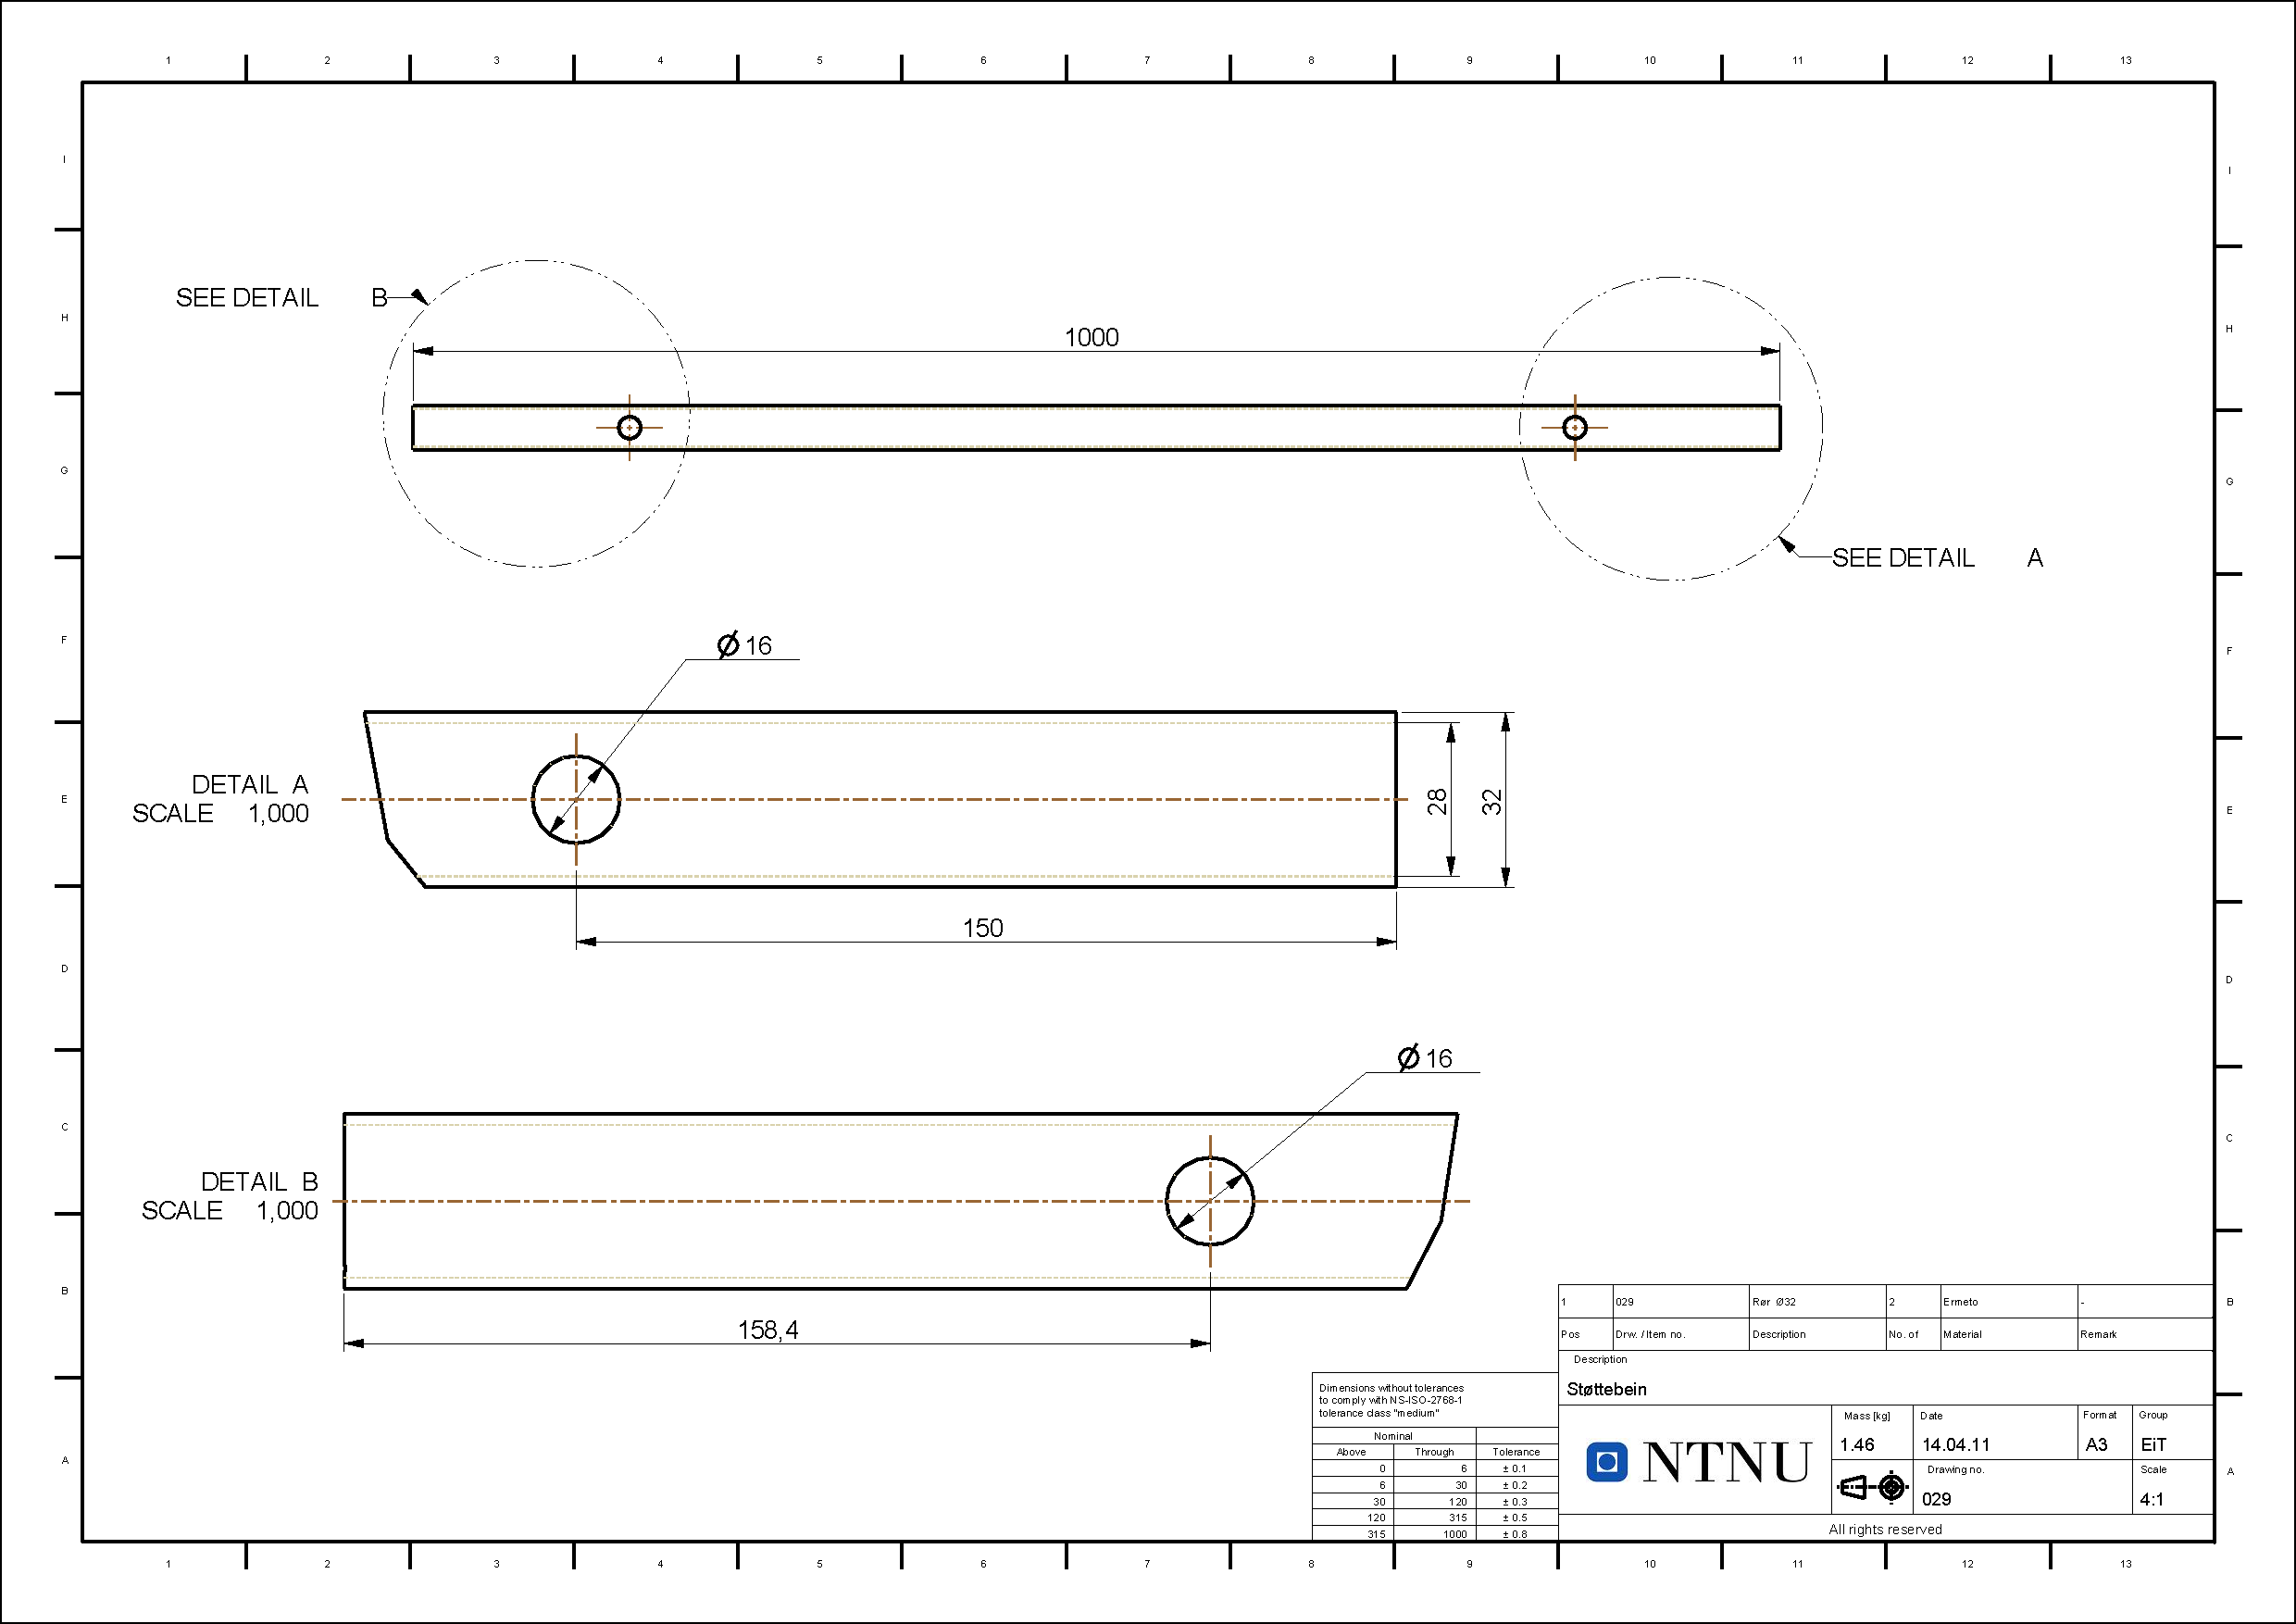
\includegraphics[angle=90, width=\textwidth]{arbeidstegninger/029}\newpage
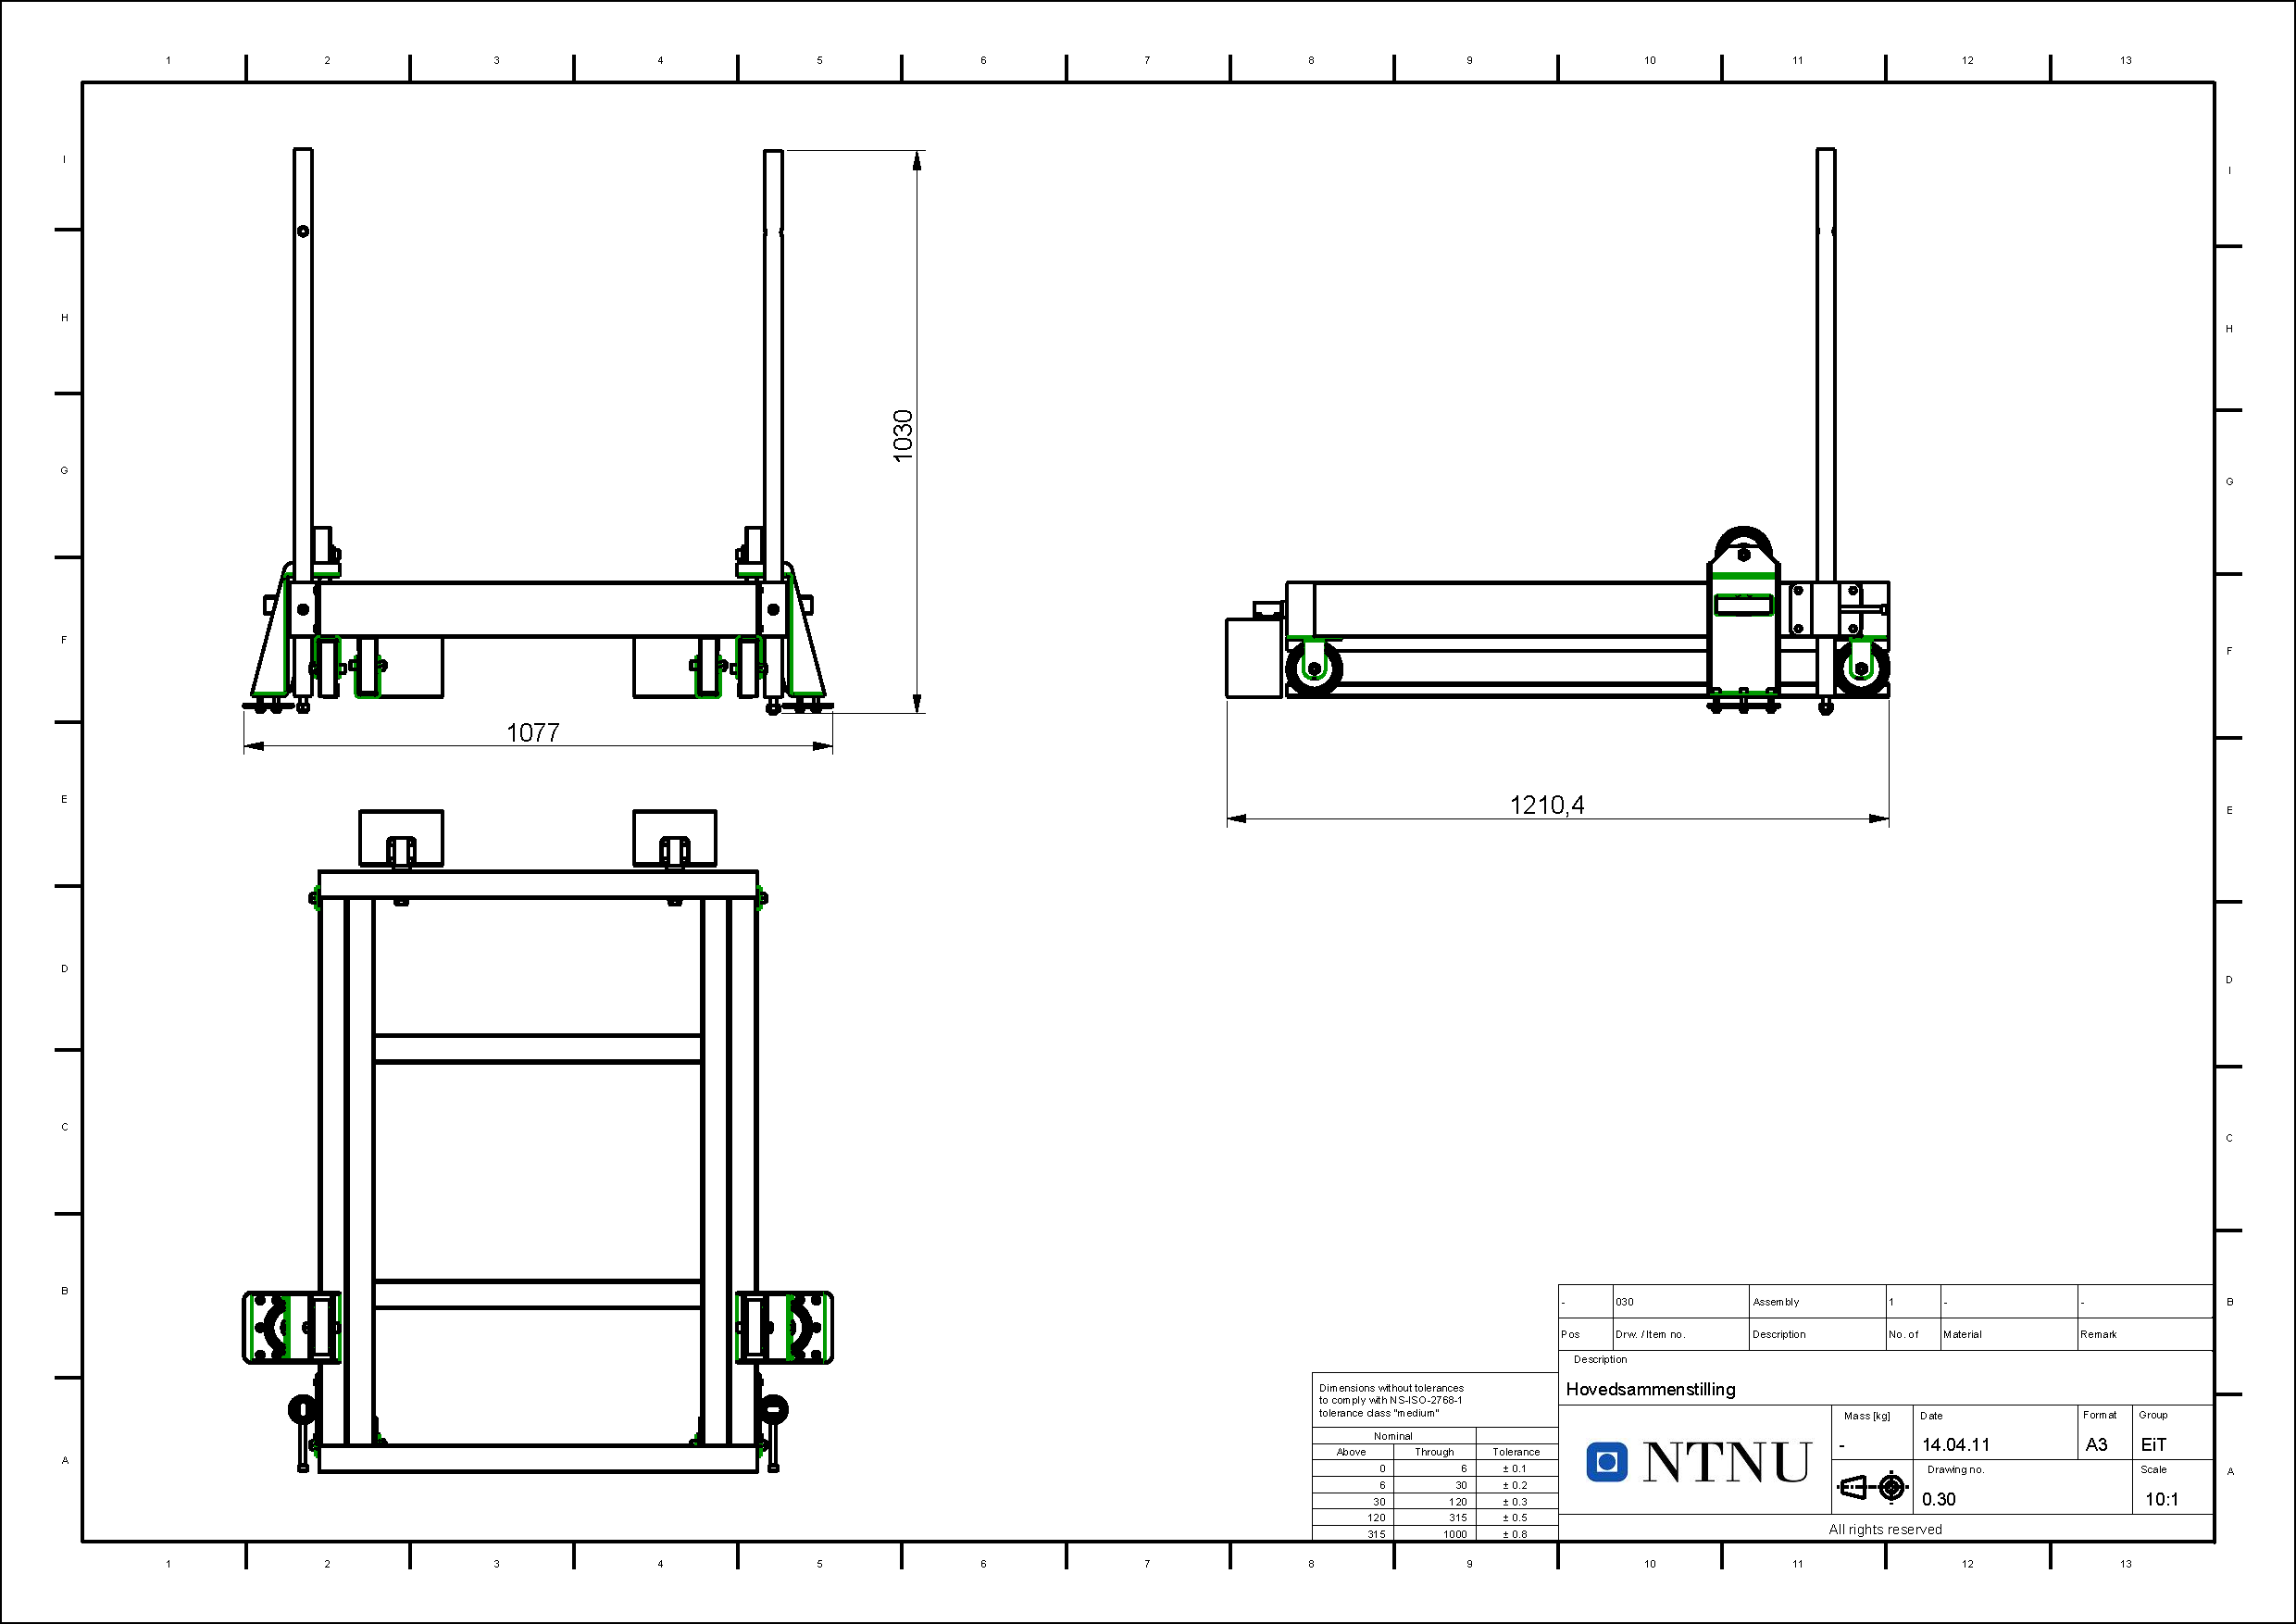
\includegraphics[angle=90, width=\textwidth]{arbeidstegninger/030}\newpage
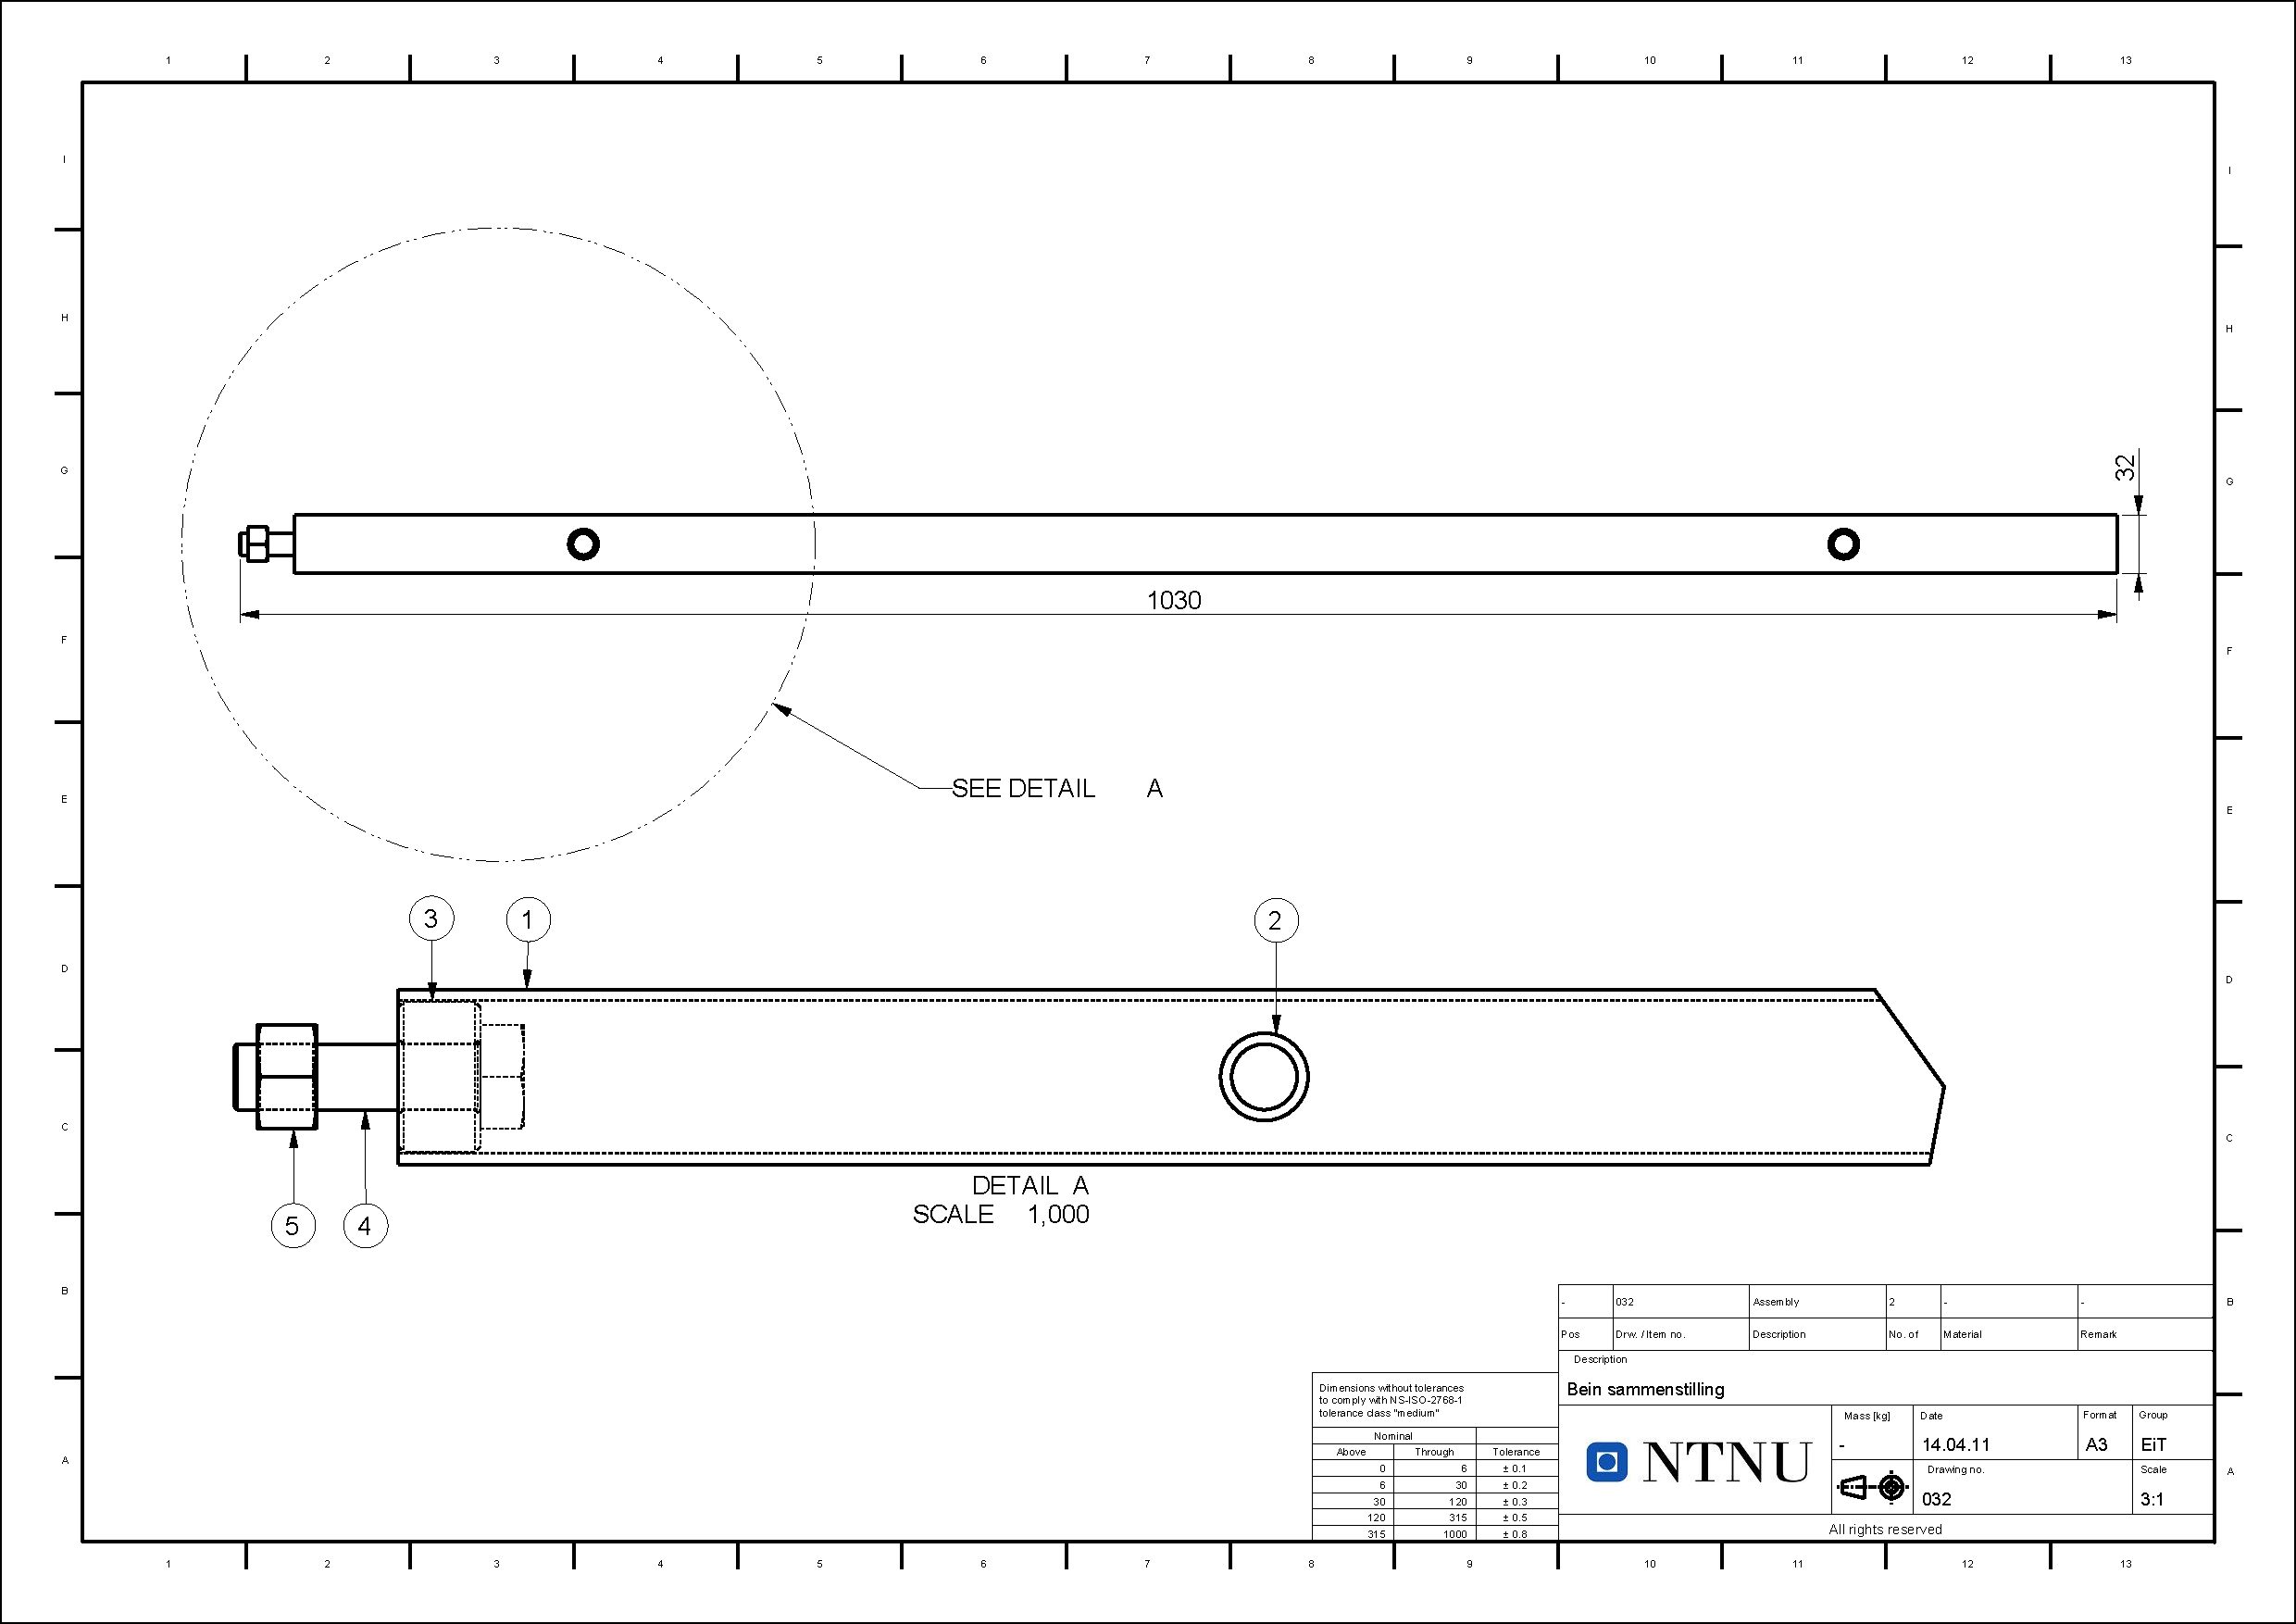
\includegraphics[angle=90, width=\textwidth]{arbeidstegninger/032}\newpage
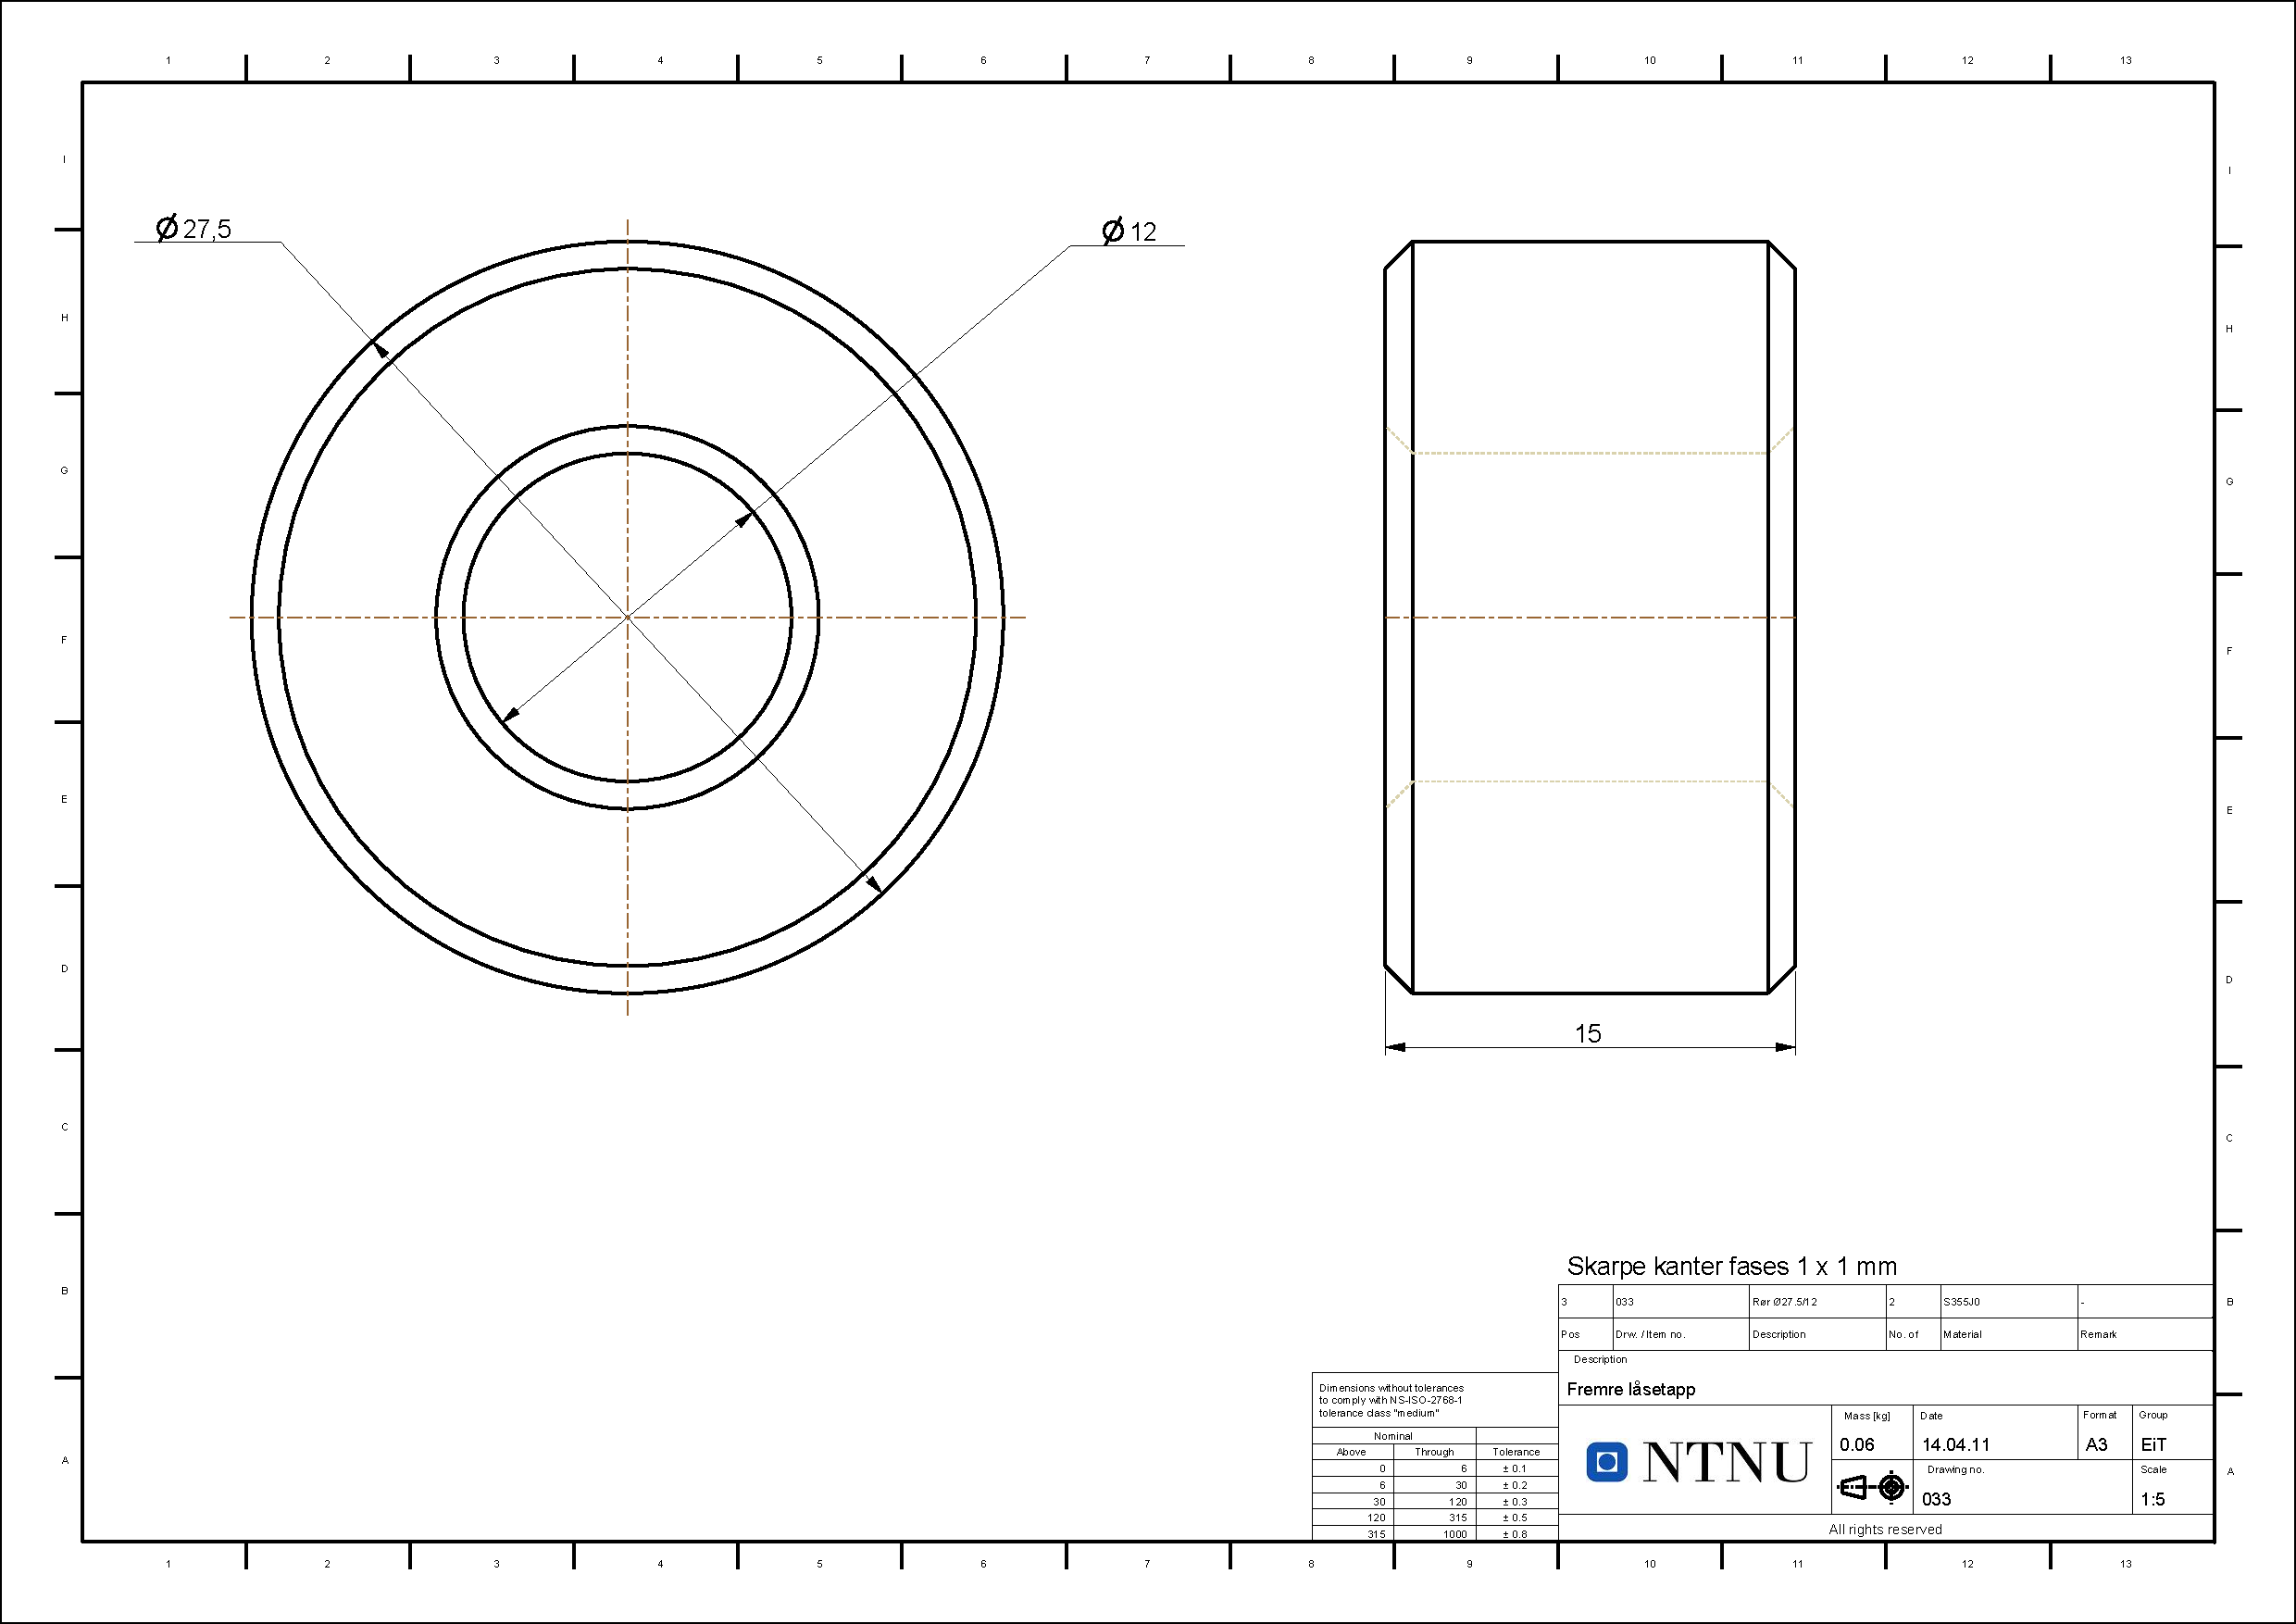
\includegraphics[angle=90, width=\textwidth]{arbeidstegninger/033}\newpage
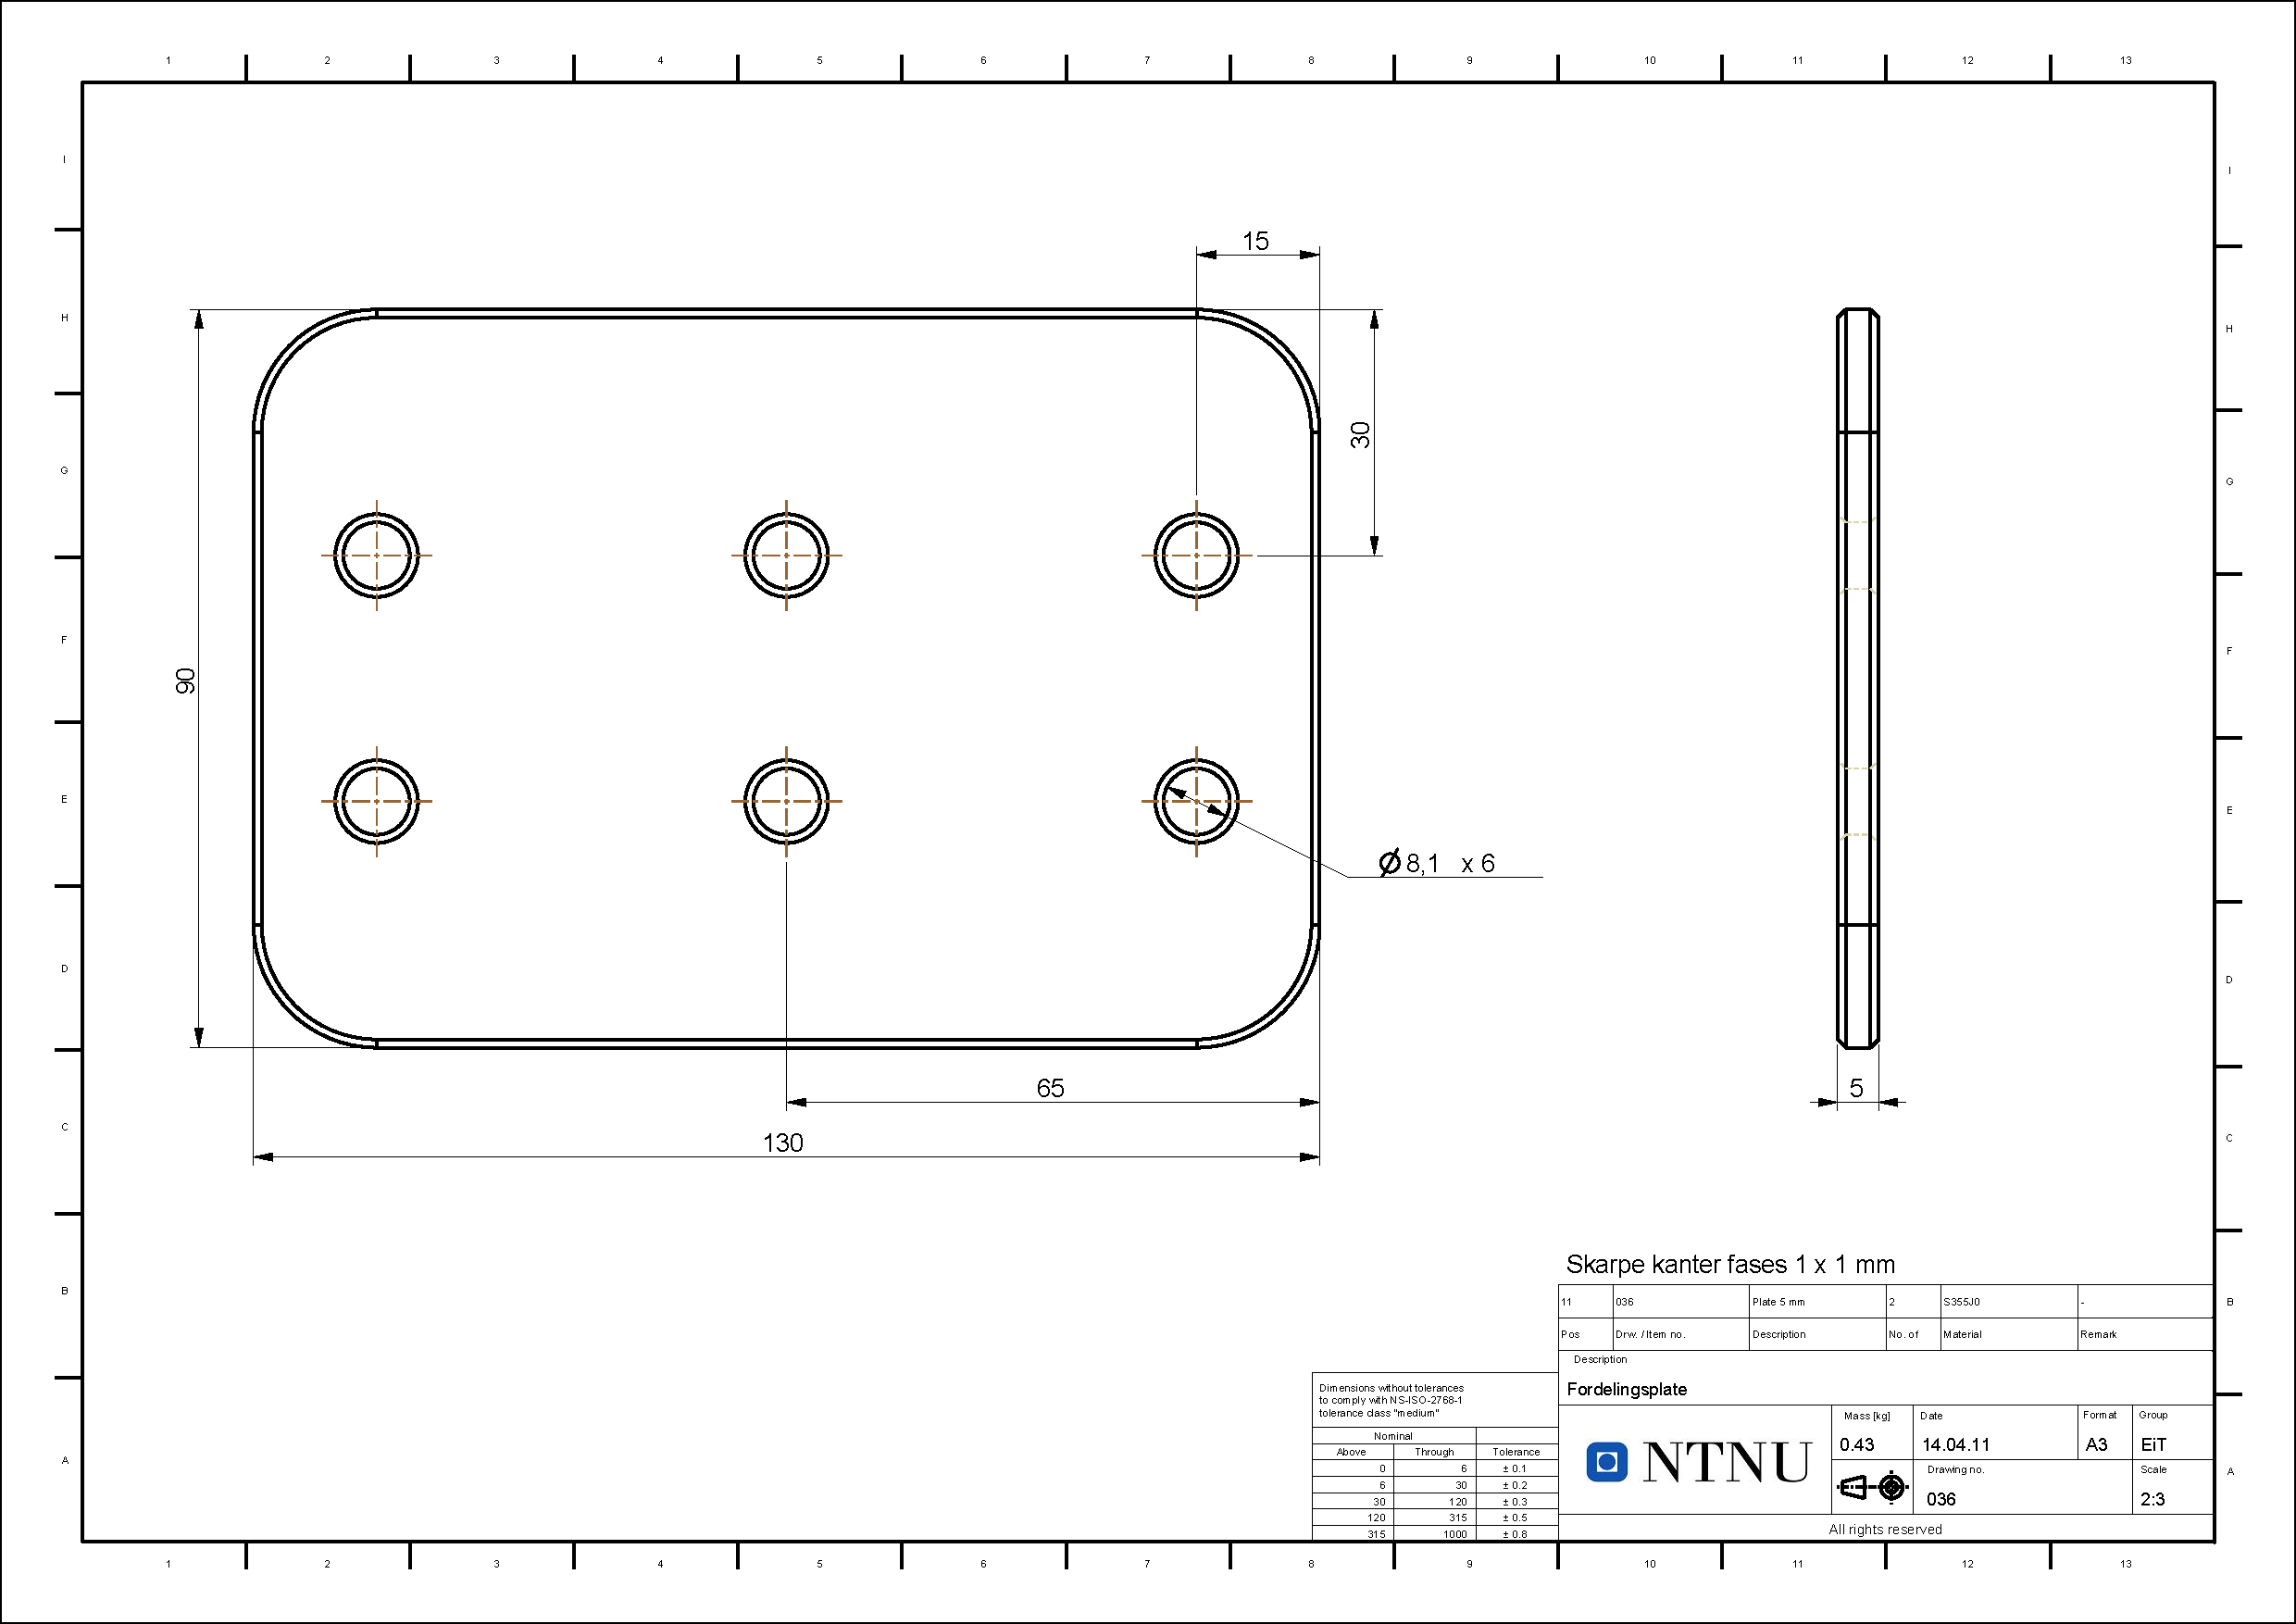
\includegraphics[angle=90, width=\textwidth]{arbeidstegninger/036}\newpage
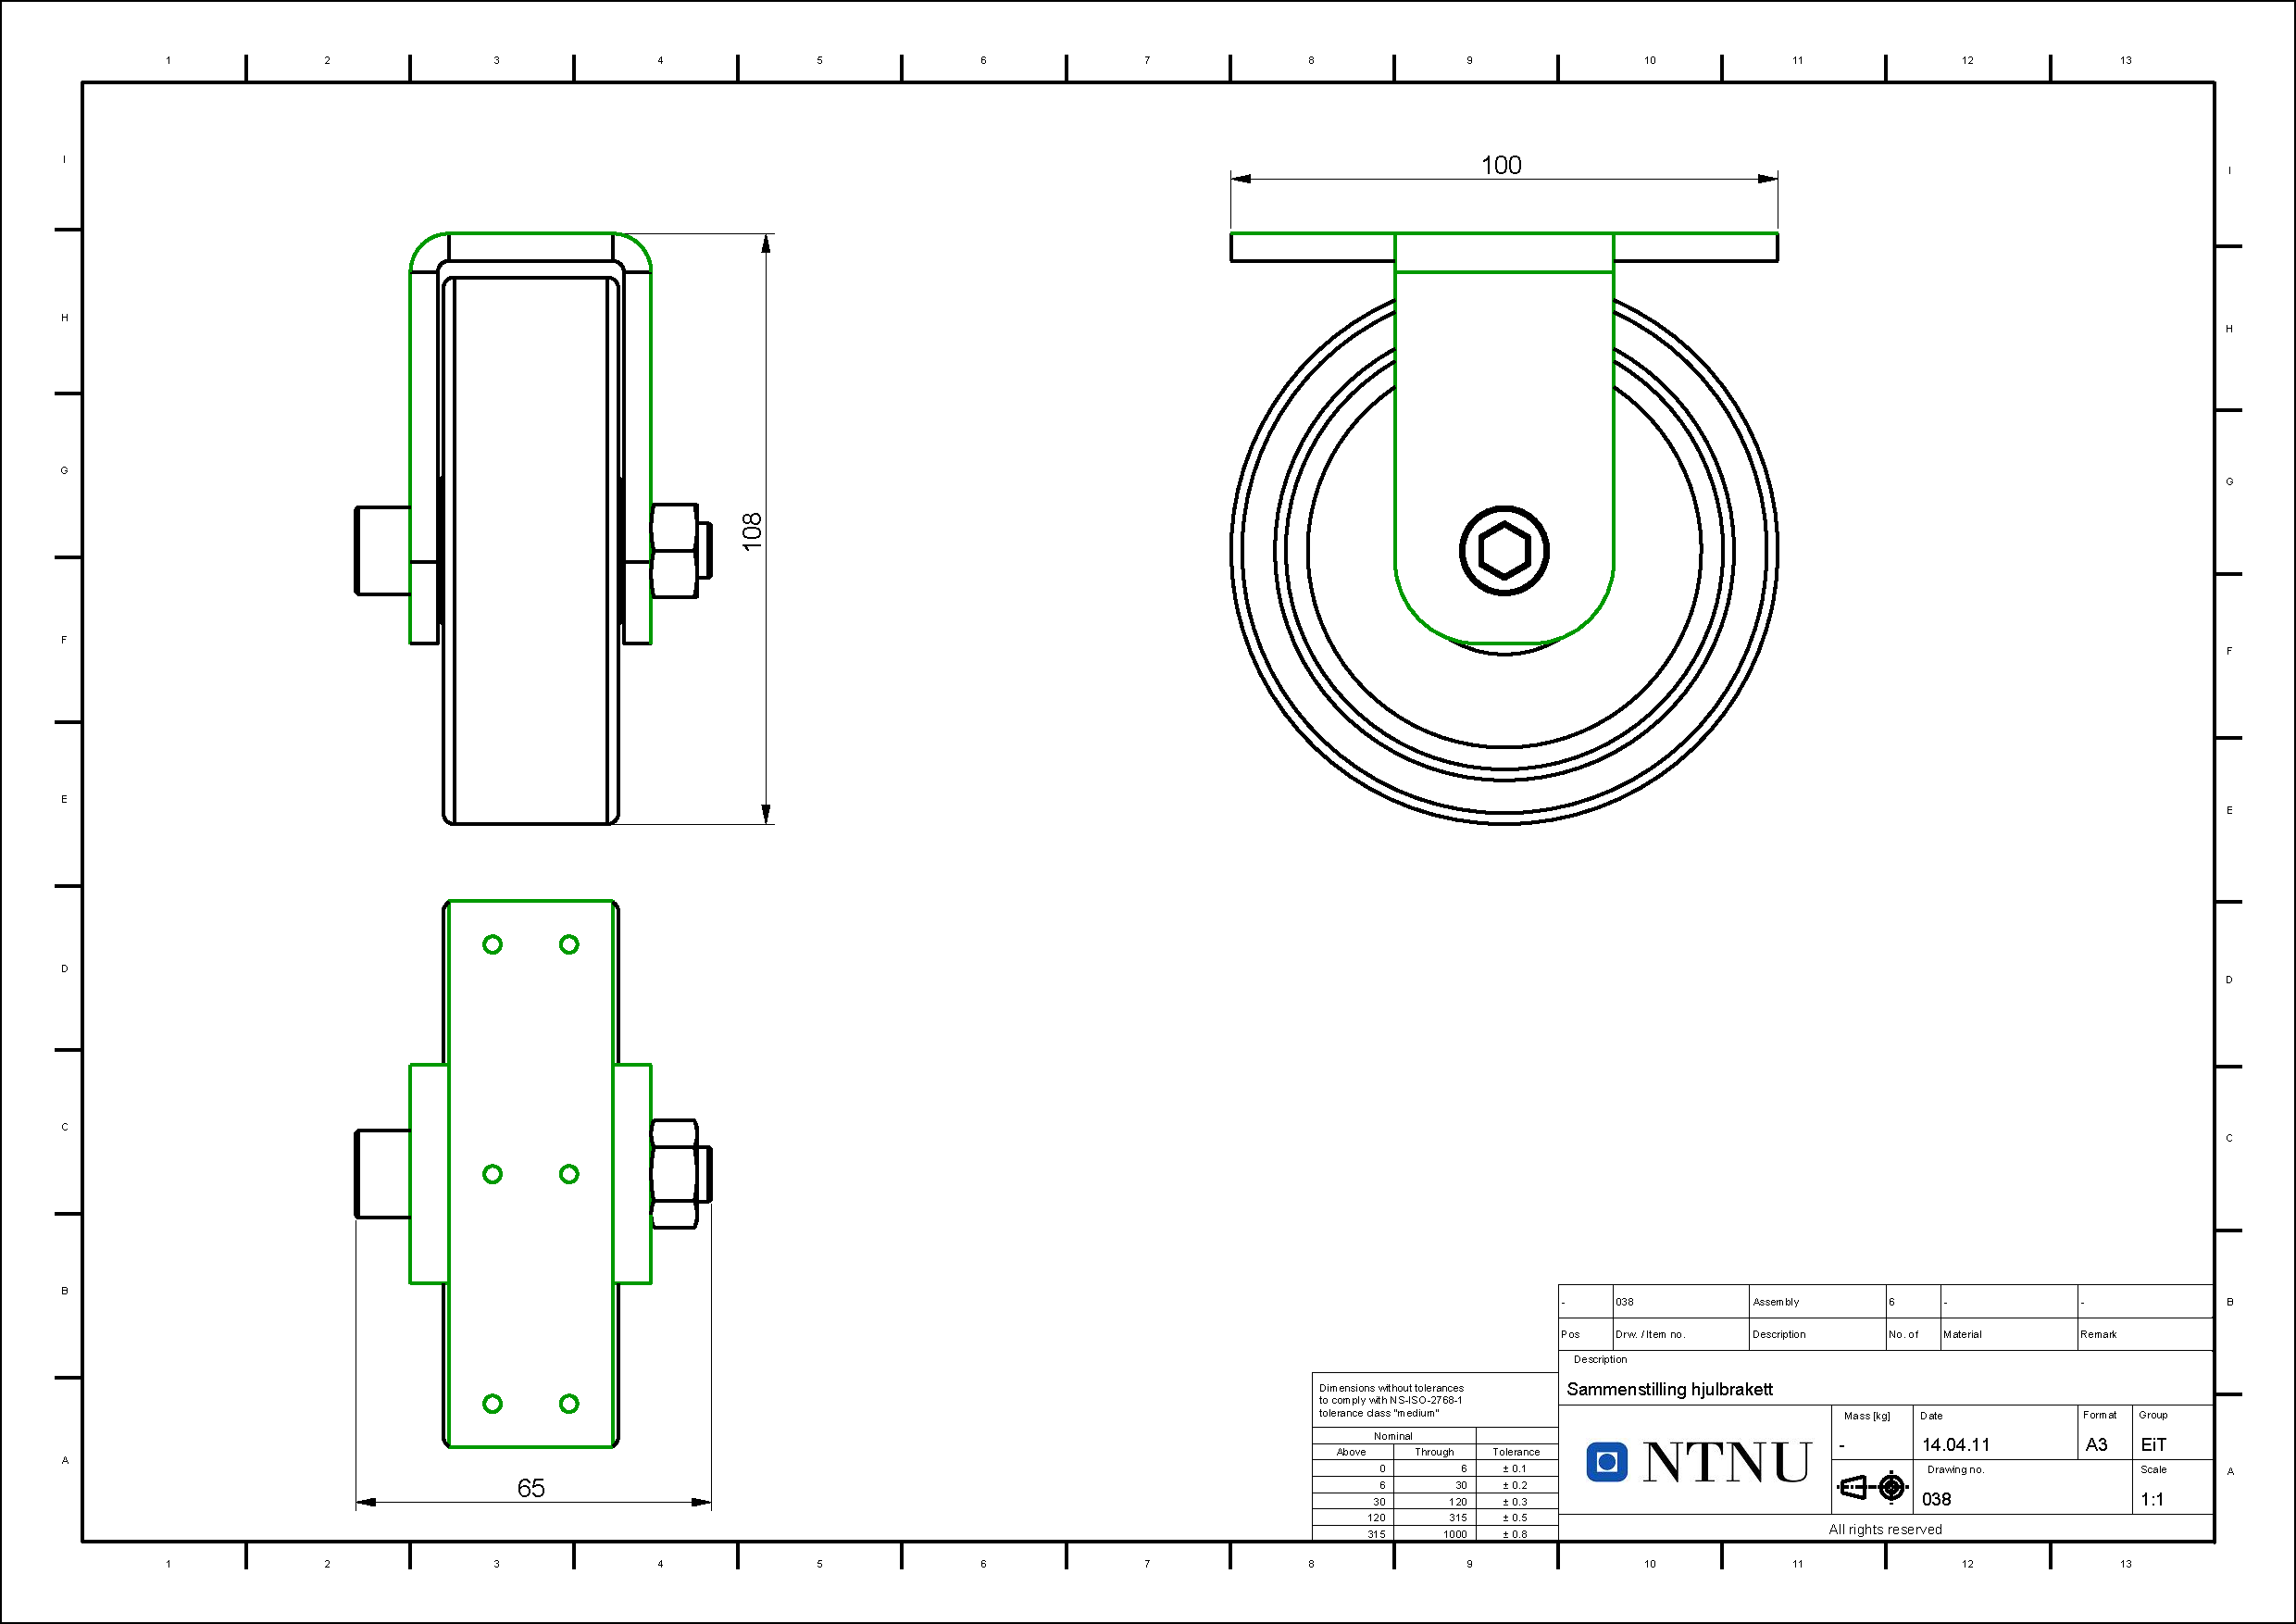
\includegraphics[angle=90, width=\textwidth]{arbeidstegninger/038}\newpage
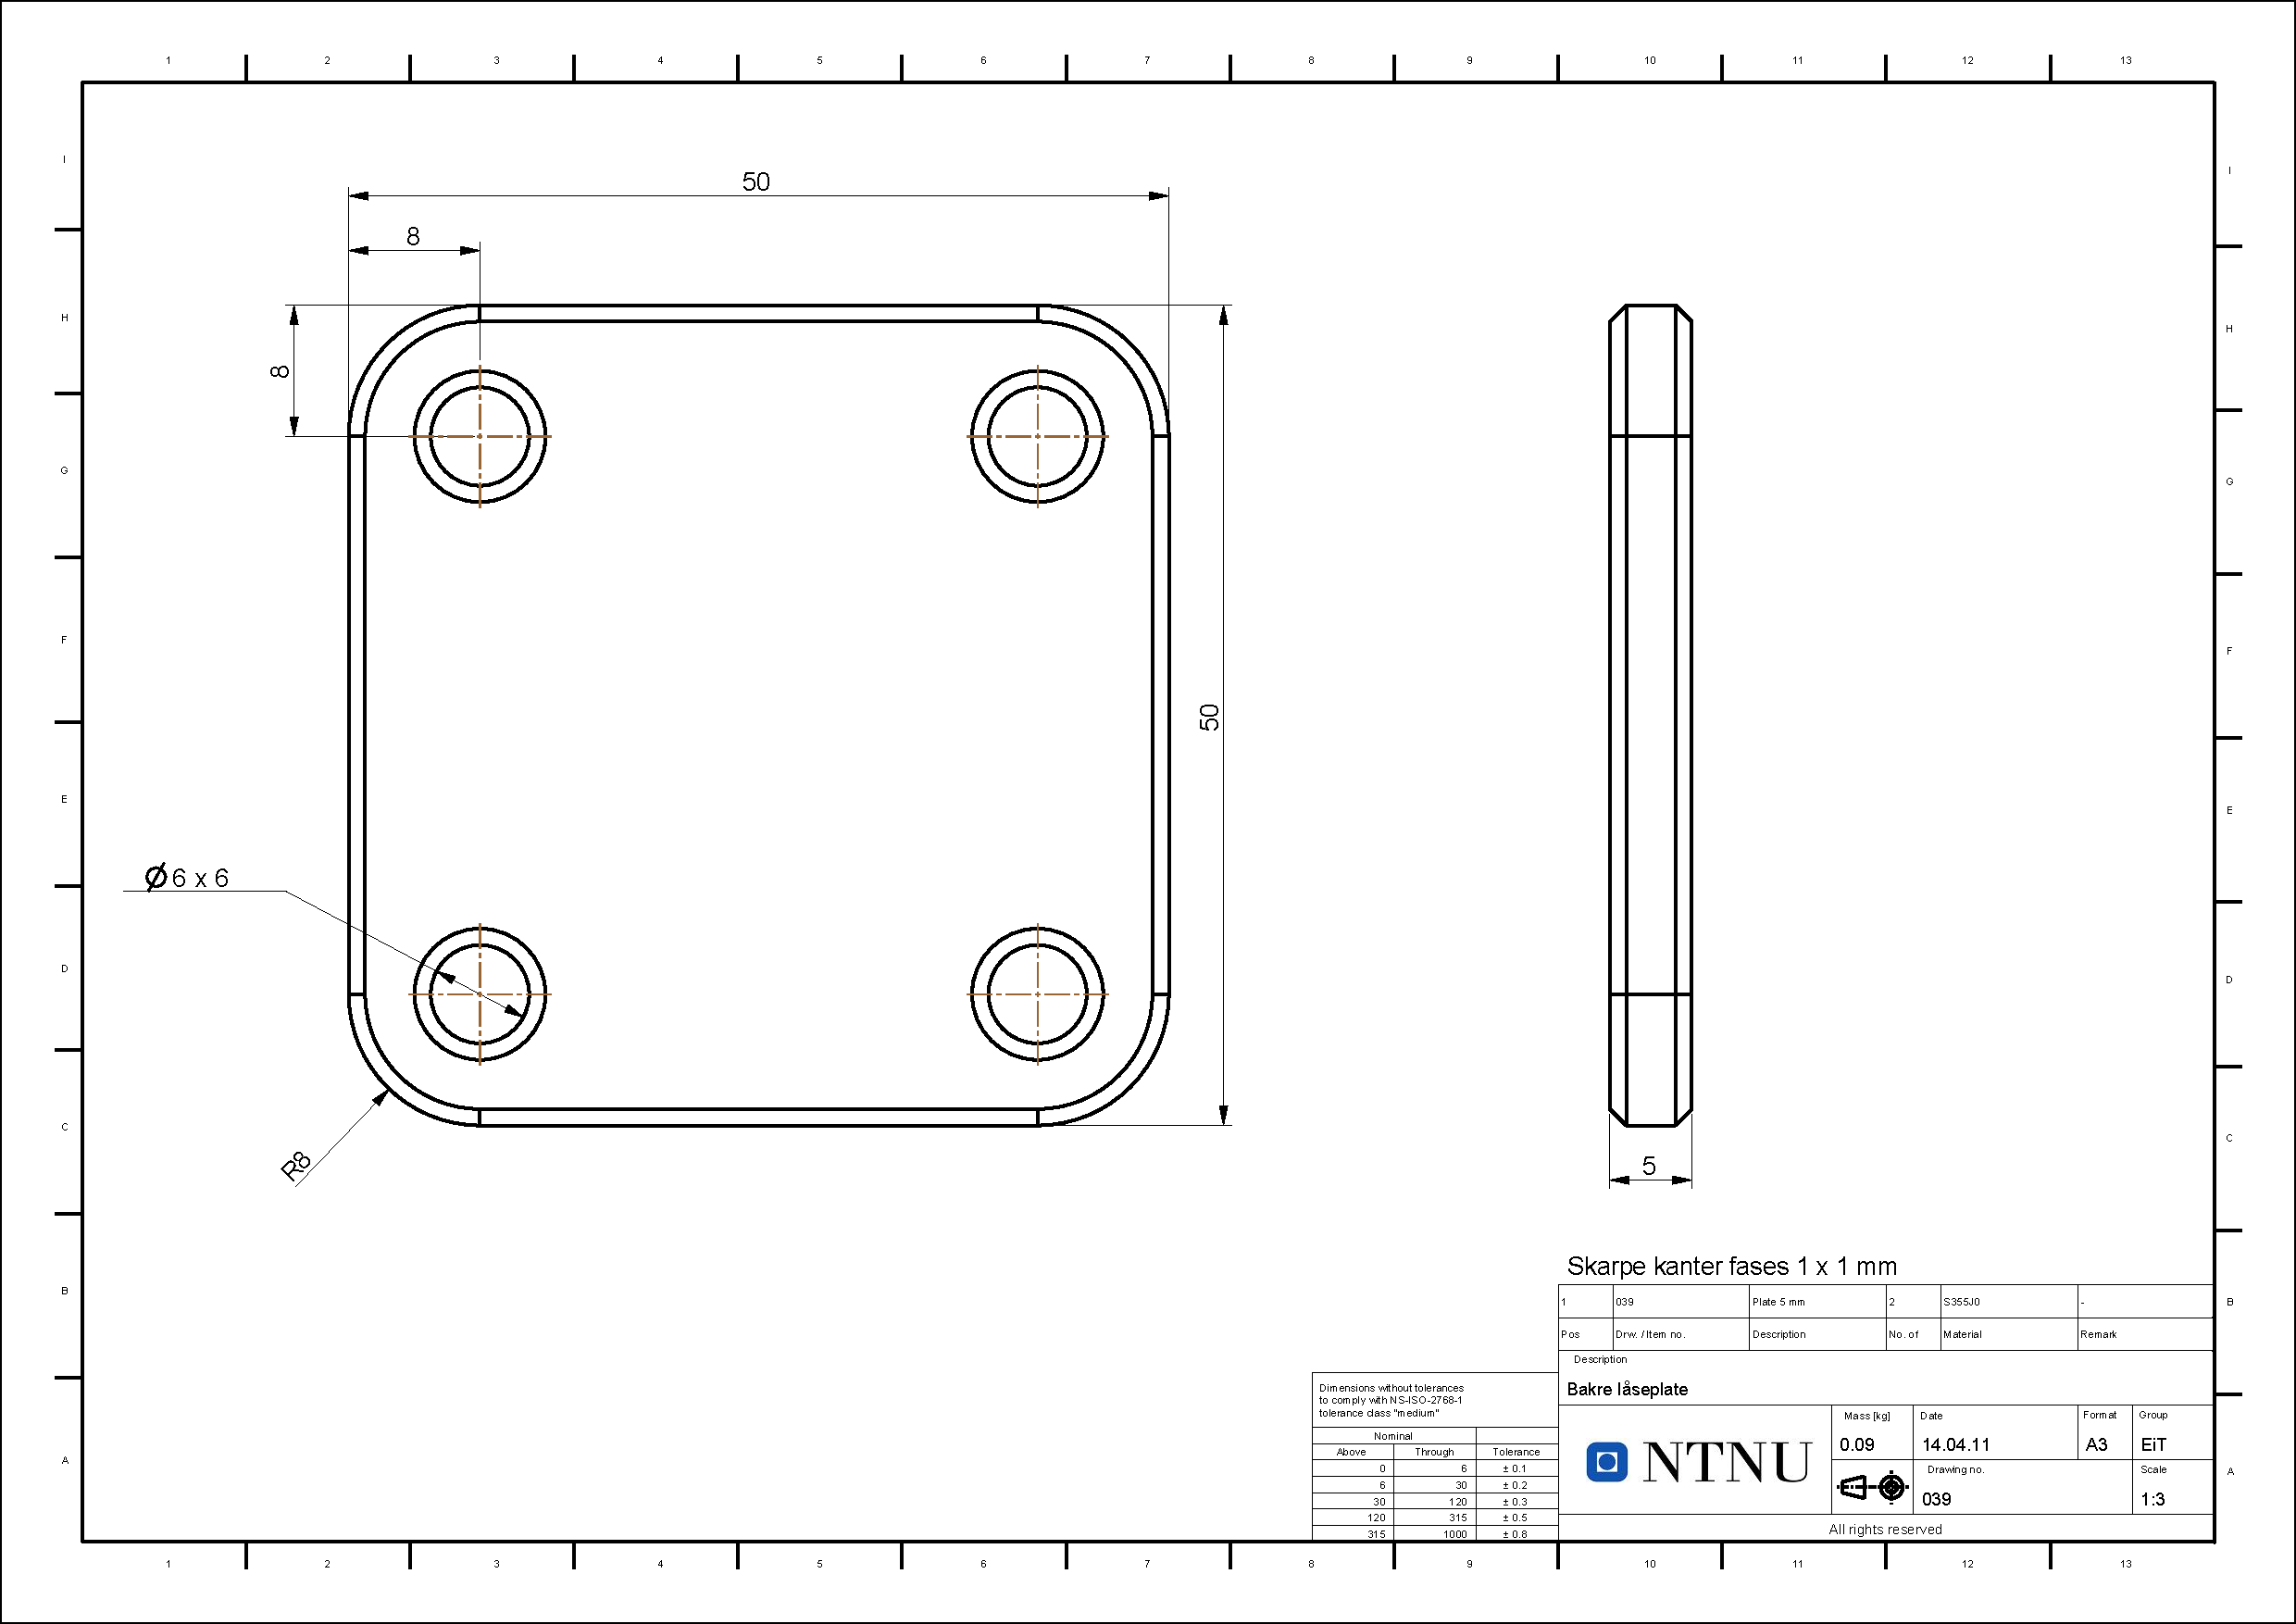
\includegraphics[angle=90, width=\textwidth]{arbeidstegninger/039}






\clearpage 
\bibliographystyle{plain} 
\bibliography{bibl} 

\end{document}
